%# -*- coding: utf-8-unix -*-
\documentclass{gbook}

\usepackage{tikz}
\usetikzlibrary{backgrounds}
\usetikzlibrary{arrows,shapes}
\usetikzlibrary{tikzmark}
\usetikzlibrary{calc}

\usepackage{amsmath}
\usepackage{amsthm}
\usepackage{amssymb}
\usepackage{mathtools, nccmath}
\usepackage{wrapfig}
\usepackage{comment}

% To generate dummy text
\usepackage{blindtext}


%color
%\usepackage[dvipsnames]{xcolor}
% \usepackage{xcolor}


%\usepackage[pdftex]{graphicx}
\usepackage{graphicx}
% declare the path(s) for graphic files
%\graphicspath{{../Figures/}}

% extensions so you won't have to specify these with
% every instance of \includegraphics
% \DeclareGraphicsExtensions{.pdf,.jpeg,.png}

% for custom commands
\usepackage{xspace}

% table alignment
\usepackage{array}
\usepackage{ragged2e}
\newcolumntype{P}[1]{>{\RaggedRight\hspace{0pt}}p{#1}}
\newcolumntype{X}[1]{>{\RaggedRight\hspace*{0pt}}p{#1}}

% color box
\usepackage{tcolorbox}


% for tikz
\usepackage{tikz}
%\usetikzlibrary{trees}
\usetikzlibrary{arrows,shapes,positioning,shadows,trees,mindmap}
% \usepackage{forest}
\usepackage[edges]{forest}
\usetikzlibrary{arrows.meta}
\colorlet{linecol}{black!75}
\usepackage{xkcdcolors} % xkcd colors


% for colorful equation
\usepackage{tikz}
\usetikzlibrary{backgrounds}
\usetikzlibrary{arrows,shapes}
\usetikzlibrary{tikzmark}
\usetikzlibrary{calc}
% Commands for Highlighting text -- non tikz method
\newcommand{\highlight}[2]{\colorbox{#1!17}{$\displaystyle #2$}}
%\newcommand{\highlight}[2]{\colorbox{#1!17}{$#2$}}
\newcommand{\highlightdark}[2]{\colorbox{#1!47}{$\displaystyle #2$}}

% my custom colors for shading
\colorlet{mhpurple}{Plum!80}


% Commands for Highlighting text -- non tikz method
\renewcommand{\highlight}[2]{\colorbox{#1!17}{#2}}
\renewcommand{\highlightdark}[2]{\colorbox{#1!47}{#2}}

% Some math definitions
\newcommand{\lap}{\mathrm{Lap}}
\newcommand{\pr}{\mathrm{Pr}}

\newcommand{\Tset}{\mathcal{T}}
\newcommand{\Dset}{\mathcal{D}}
\newcommand{\Rbound}{\widetilde{\mathcal{R}}}

\begin{document}

\everymath{\displaystyle}

\setlength{\lineskip}{2.5pt}
\setlength{\lineskiplimit}{2.5pt}

%# -*- coding: utf-8-unix -*-
\thispagestyle{empty}
\begin{tikzpicture}[overlay,remember picture,font=\sffamily\bfseries]
\draw[ultra thick,c4,name path=big arc] ([xshift=-2mm]current page.north) arc(150:285:11)
coordinate[pos=0.225] (x0);
\begin{scope}
\clip ([xshift=-2mm]current page.north) arc(150:285:11) --(current page.north
east);
\fill[c4!50,opacity=0.25] ([xshift=4.55cm]x0) circle (4.55);
\fill[c4!50,opacity=0.25] ([xshift=3.4cm]x0) circle (3.4);
\fill[c4!50,opacity=0.25] ([xshift=2.25cm]x0) circle (2.25);
\draw[ultra thick,c4!50] (x0) arc(-90:30:6.5);
\draw[ultra thick,c4] (x0) arc(90:-30:8.75);
\draw[ultra thick,c4!50,name path=arc1] (x0) arc(90:-90:4.675);
\draw[ultra thick,c4!50] (x0) arc(90:-90:2.875);
\path[name intersections={of=big arc and arc1,by=x1}];
\draw[ultra thick,c4,name path=arc2] (x1) arc(135:-20:4.75);
\draw[ultra thick,c4!50] (x1) arc(135:-20:8.75);
\path[name intersections={of=big arc and arc2,by={aux,x2}}];
\draw[ultra thick,c4!50] (x2) arc(180:50:2.25);
\end{scope} 
\path[decoration={text along path,text color=c4,
	raise = -2.8ex,
	text  along path,
	text = {|\sffamily\bfseries|Build:\today},
	text align = center,
},
decorate
] ([xshift=-2mm]current page.north) arc(150:245:11);
%
\begin{scope}
\path[clip,postaction={fill=c3}]
([xshift=2cm,yshift=-8cm]current page.center) rectangle ++ (4.2,7.7);
\fill[c2] ([xshift=0.5cm,yshift=-8cm]current page.center)
([xshift=0.5cm,yshift=-8cm]current page.center)  arc(180:60:2)
|- ++ (-3,6) --cycle;
\draw[ultra thick,c4] ([xshift=-1.5cm,yshift=-8cm]current page.center) 
arc(180:0:2);
\draw[ultra thick,c4] ([xshift=0.5cm,yshift=-8cm]current page.center) 
arc(180:0:2);
\draw[ultra thick,c4] ([xshift=2.5cm,yshift=-8cm]current page.center) 
arc(180:0:2);
\draw[ultra thick,c4] ([xshift=4.5cm,yshift=-8cm]current page.center) 
arc(180:0:2);
\end{scope}
%
\fill[c1] ([xshift=2cm,yshift=-8cm]current page.center) rectangle ++ (-13.7,7.7);
\node[text=white,anchor=west,scale=3,inner sep=0pt] at
([xshift=-10.55cm,yshift=-3cm]current page.center) {\enspace 高中物理二级结论随笔};
\node[text=white,anchor=west,scale=2,inner sep=0pt] at
([xshift=-4.5cm,yshift=-5.5cm]current page.center) {By Guotao He};
\end{tikzpicture} 

\newpage

\pagenumbering{Roman} %设置罗马数字页码

\setcounter{page}{1}

\section*{前言}

\phantomsection\addcontentsline{toc}{chapter}{前言}

本书采用\LaTeX 语言编写,使用Lua\LaTeX 在TexPage、GitHub Actions以及一台装有Tex Live 2021的Android平板三个平台上完成编译(因此选用Lua\LaTeX,此渲染引擎对系统字库要求较小,便于在Android设备中运行)。
~\\

\begin{minipage}[b]{0.62\linewidth}
本书在GitHub上开源,GitHub项目链接:

\url{https://github.com/GHe0000/GHe_Book} 
\end{minipage}
\hfill
\begin{minipage}[b]{0.1\linewidth}
\qrcode[1cm]{https://github.com/GHe0000/GHe_Book}
\end{minipage}
~\\

借助GitHub Actions,每次在GitHub上Push都会自动进行PDF的编译和发布,但此PDF经过校验,可能会有错误。你可以在此链接下载GitHub Actions自动编译的最新版本:\url{https://ghe0000.github.io/GHe_Book/main.pdf}

本书遵循CC 4.0 BY-NC协议\footnote{你可以在此找到该协议的完整描述:\url{https://creativecommons.org/licenses/by-nc/4.0/legalcode.zh-Hans}}共享,简而言之,您可以自由地:
\begin{itemize}
    \item 共享 —— 在任何媒介以任何形式复制、发行本作品
    \item 演绎 —— 修改、转换或以本作品为基础进行创作
\end{itemize}

惟须遵守下列条件:
\begin{itemize}
    \item 署名
    \item 非商业性使用
    \item 没有附加限制 —— 您不得限制其他人做许可协议允许的事情
\end{itemize}
~\\

本书自2022年11月26日开始编写,至2023年3月18日完稿第一版。

当然,这本书仍旧有许多不足,如结论过少,图示不清晰、不详细,结论推导不详细,表述不恰当,例题不足等等。笔者很多有意思的想法也没能在书中分享。只可惜时间不够、精力不足,目前只能以这一粗糙版本发布,望各位读者谅解。

最后,本书欢迎各位读者参与共同编写(新增内容可直接在GitHub上提交PR,也可发至下文的邮箱中,整理后会合并入本书,详情见GitHub项目链接),也欢迎各位读者询问本书有关内容,指出本书的问题、错误,提出本书的优化意见等。读者可以在GitHub issue上提出反馈,也可发送电子邮件至邮箱\url{guotao.he.0000@outlook.com}
~\\

\begin{flushright}
2020级12班

Guotao He

2023年3月18日
\end{flushright}
\newpage

\section*{书籍简介}

\phantomsection\addcontentsline{toc}{chapter}{书籍简介}

\newpage

\pagenumbering{roman} %设置罗马数字页码

\setcounter{page}{1}

\tableofcontents

\newpage

\setcounter{page}{1}

\pagenumbering{arabic} %设置拉丁数字页码

%# -*- coding: utf-8-unix -*-
%%==================================================
\tikzset{every picture/.style={line width=0.75pt}} %set default line width to 0.75pt    

\chapter{高中物理常用数据及图像}

\section{常用物理学常量}

\begin{table}[h]
\centering
\begin{threeparttable}
\begin{tabular}{l|l|l|l}
\textbf{符号} & \textbf{名称} & \textbf{精确值}\tnote{1} & \textbf{高中常用值}\\
\hline
$g$ & 重力加速度 & $9.80665 m/s^2$ & $10m/s^2$ \\
$G$ & 引力常量 & $6.67384 \times 10^{11} N \cdot m^2/kg^2$ & $6.67 \times 10^{-11} N \cdot m^2/kg^2$ \\
$e$ & 元电荷 & $1.602176565 \times 10^{-19} C$ & $1.6 \times 10^{-19} C$ \\ 
$k$ &  静电力常量 & $8987551788 N \cdot m^2 / C^2$ & $9 \times 10^{9} N \cdot m^2 /C^2$ \\
$c$ & 真空中光速 & $299792458 m/s$ & $3 \times 10^{8} m/s$ \\
$h$ & 普朗克常数 & $6.62606957 \times 10^{-34} J \cdot s$ & $6.63 \times 10^{-34} J \cdot s$ \\
\hline
\end{tabular}
\begin{tablenotes}
\item[1] 精确值参考了CODATA(2010)推荐值,可能跟高中课本有细微出入
\end{tablenotes}
\end{threeparttable}
\end{table}

\section{常用估计值}

\begin{center}
\begin{tabular}{l|l|l|l|l}
\textbf{符号} & \textbf{名称} & \textbf{估计值} & \textbf{备注} \\
\hline
$R_{earth}$ & 地球半径  & $6400 km$  & \\
$\rho_{earth}$ & 地球平均密度 & $5500 kg/m^3$ & 水密度的5.5倍 \\
$R_{sync}$ & 同步卫星轨道半径  &  & \\
$U_{m}$ & $220V$市电振幅 & $311 V$ & \\
\hline
\end{tabular}
\end{center}

\section{常用单位换算}

\section{常用小量近似}

\section{常用物理图像}

\subsection{等量同种电荷}

下图中均取电荷$q=1C$,位于$(0.5m,0)$、$(-0.5m,0)$

\begin{figure}[H]
\begin{minipage}[b]{0.4\linewidth}
\centering
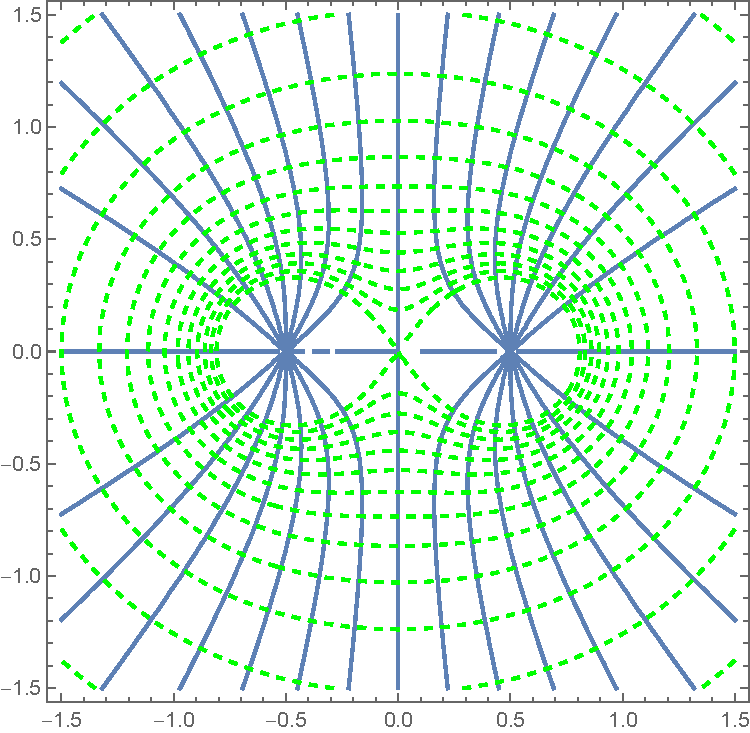
\includegraphics[width=\textwidth]{pic_data/T/dltzdh_p1.pdf}
\caption{电场线与等距等势面}
\end{minipage}
\hfill
\begin{minipage}[b]{0.4\linewidth}
\centering
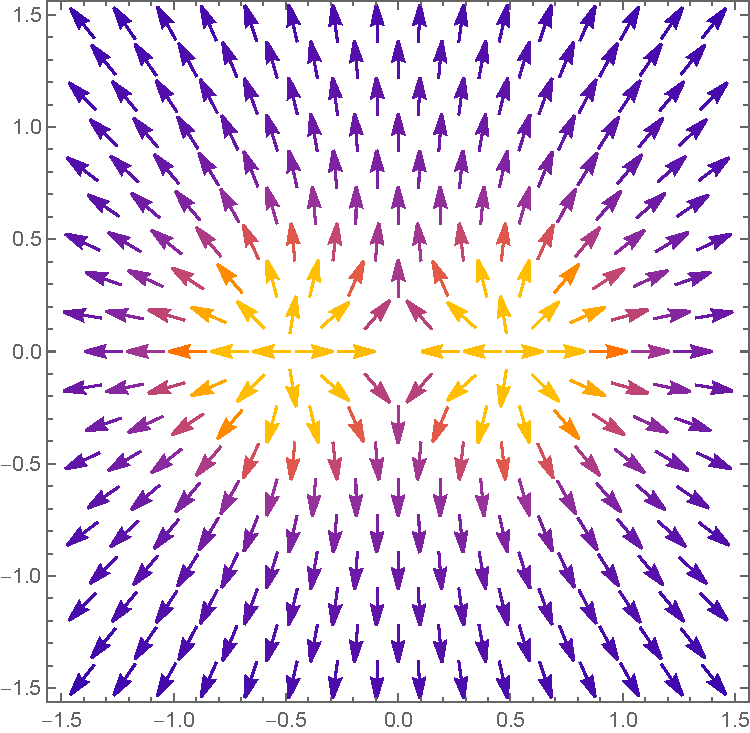
\includegraphics[width=\textwidth]{pic_data/T/dltzdh_p2.pdf}
\caption{电场场强与方向\protect \footnotemark}
\end{minipage}
\end{figure}
\footnotetext{箭头颜色表示场强,颜色越亮场强越大,下同}

\begin{figure}[H]
\begin{minipage}[b]{0.4\linewidth}
\centering
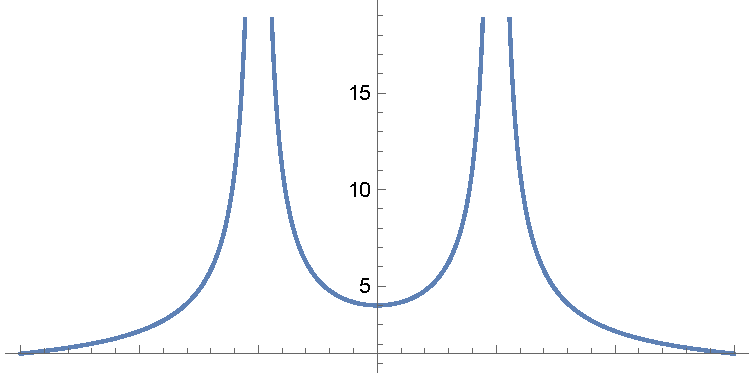
\includegraphics[width=\textwidth]{pic_data/T/phix.pdf}
\caption{沿$x$轴电势($\phi - x$图)}
\end{minipage}
\hfill
\begin{minipage}[b]{0.4\linewidth}
\centering
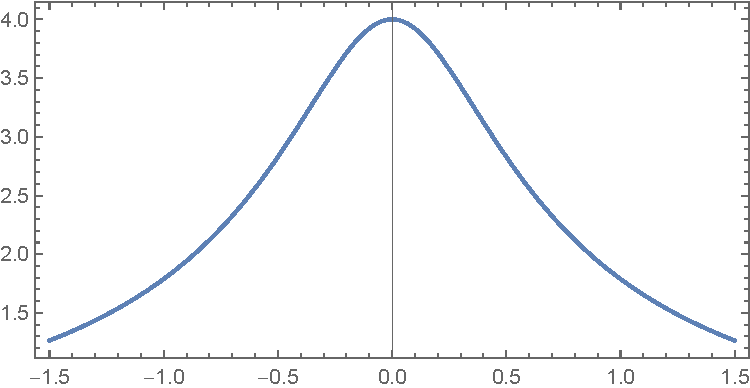
\includegraphics[width=\textwidth]{pic_data/T/phiy.pdf}
\caption{沿$y$轴电势($\phi - y$图)}
\end{minipage}
\end{figure}

\begin{figure}[H]
\begin{minipage}[b]{0.4\linewidth}
\centering
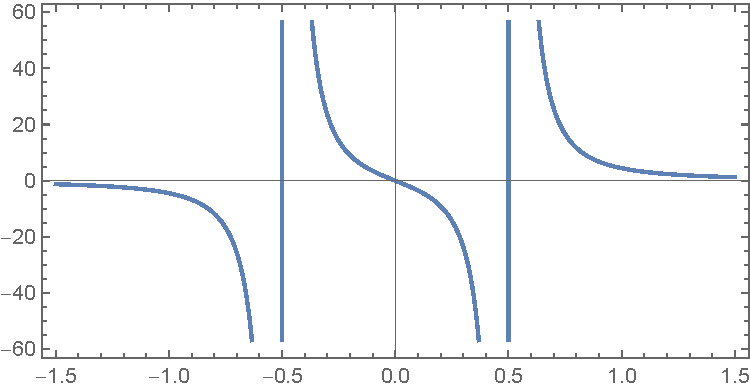
\includegraphics[width=\textwidth]{pic_data/T/Ex-x.pdf}
\caption{沿$x$轴$x$方向电场($E_x - x$图)}
\end{minipage}
\hfill
\begin{minipage}[b]{0.4\linewidth}
\centering
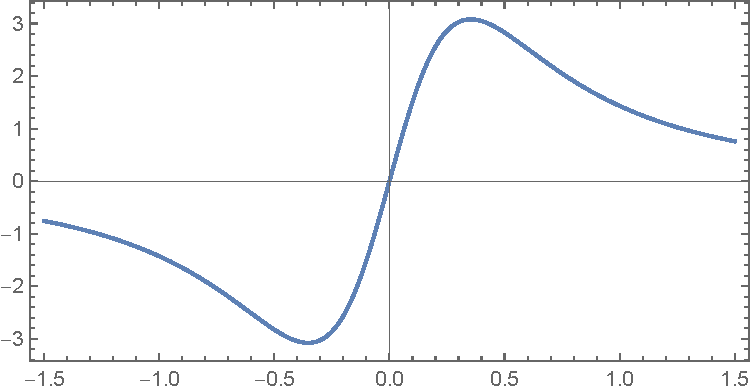
\includegraphics[width=\textwidth]{pic_data/T/Ey-y.pdf}
\caption{沿$y$轴$y$方向电场($E_y - y$图)}
\end{minipage}
\end{figure}

\subsection{等量异种电荷}

下图中取电荷$q=1C$,位于$(-0.5m,0)$;电荷$q=-1C$,位于$(0.5m,0)$

\begin{figure}[H]
\begin{minipage}[b]{0.4\linewidth}
\centering
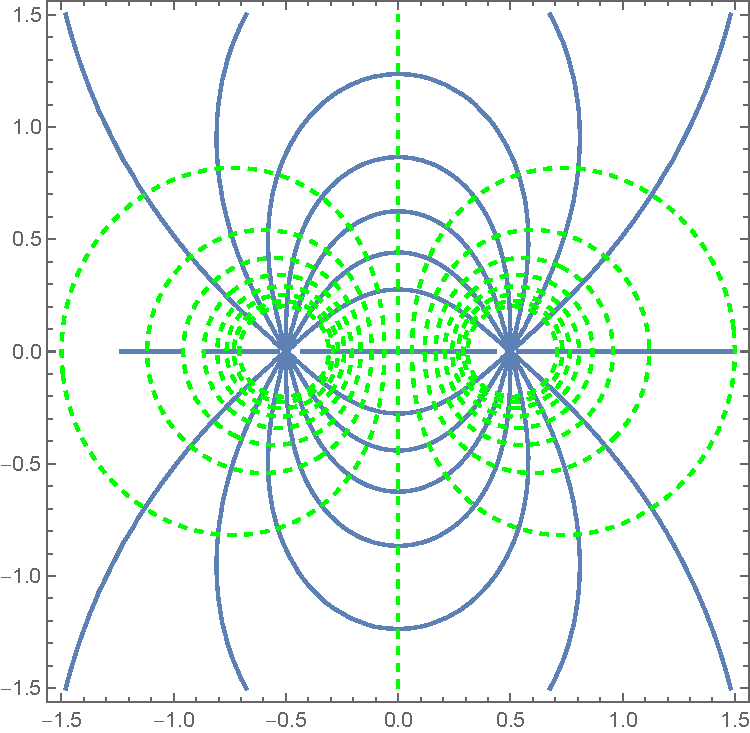
\includegraphics[width=\textwidth]{pic_data/Y/dlyzdh_p1.pdf}
\caption{电场线与等距等势面}
\end{minipage}
\hfill
\begin{minipage}[b]{0.4\linewidth}
\centering
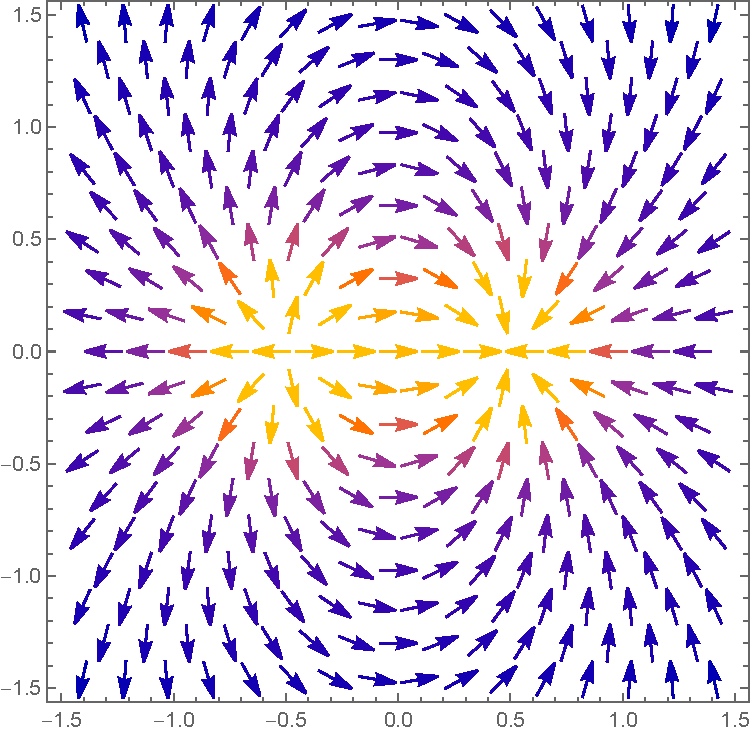
\includegraphics[width=\textwidth]{pic_data/Y/dlyzdh_p2.pdf}
\caption{电场场强与方向}
\end{minipage}
\end{figure}

\begin{figure}[H]
\begin{minipage}[b]{0.4\linewidth}
\centering
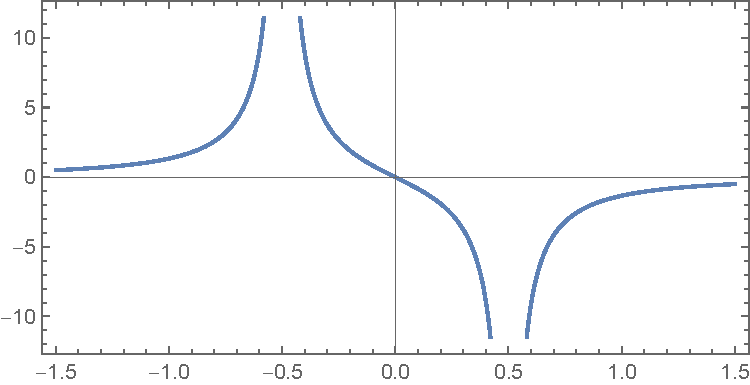
\includegraphics[width=\textwidth]{pic_data/Y/phix.pdf}
\caption{沿$x$轴电势($\phi - x$图)}
\end{minipage}
\hfill
\begin{minipage}[b]{0.4\linewidth}
\centering
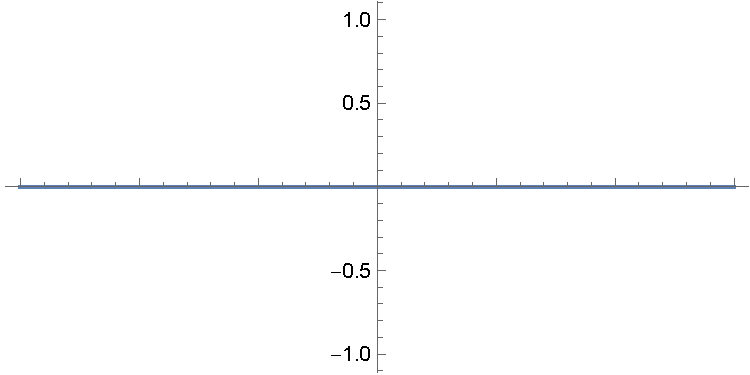
\includegraphics[width=\textwidth]{pic_data/Y/phiy.pdf}
\caption{沿$y$轴电势($\phi - y$图)}
\end{minipage}
\end{figure}

\begin{figure}[H]
\begin{minipage}[b]{0.4\linewidth}
\centering
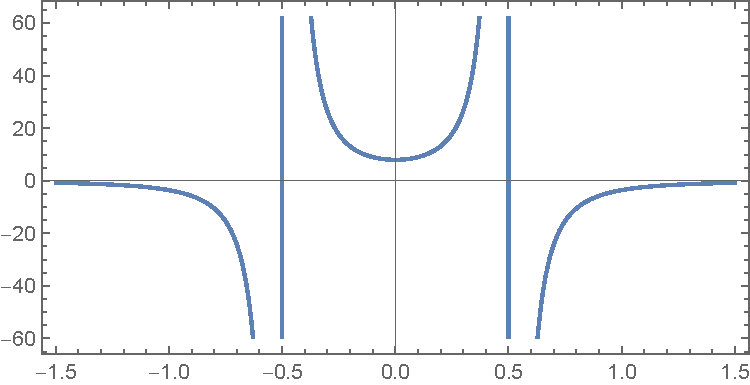
\includegraphics[width=\textwidth]{pic_data/Y/Ex-x.pdf}
\caption{沿$x$轴$x$方向电场($E_x - x$图)}
\end{minipage}
\hfill
\begin{minipage}[b]{0.4\linewidth}
\centering
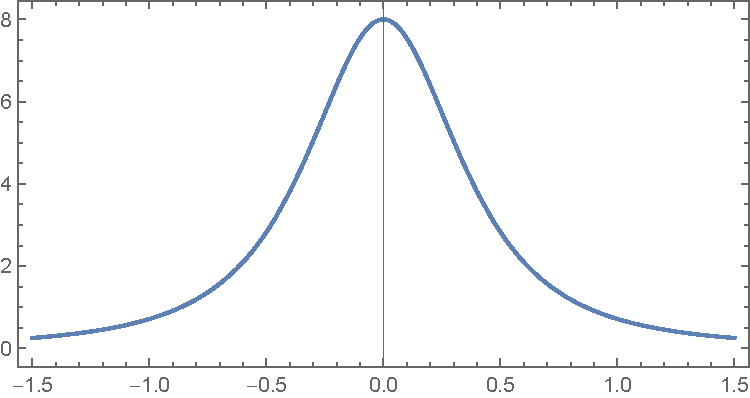
\includegraphics[width=\textwidth]{pic_data/Y/Ex-y.pdf}
\caption{沿$y$轴$x$方向电场($E_x - y$图)}
\end{minipage}
\end{figure}

\subsection{磁场}

\begin{figure}[H]
\begin{minipage}[b]{0.4\linewidth}
\centering
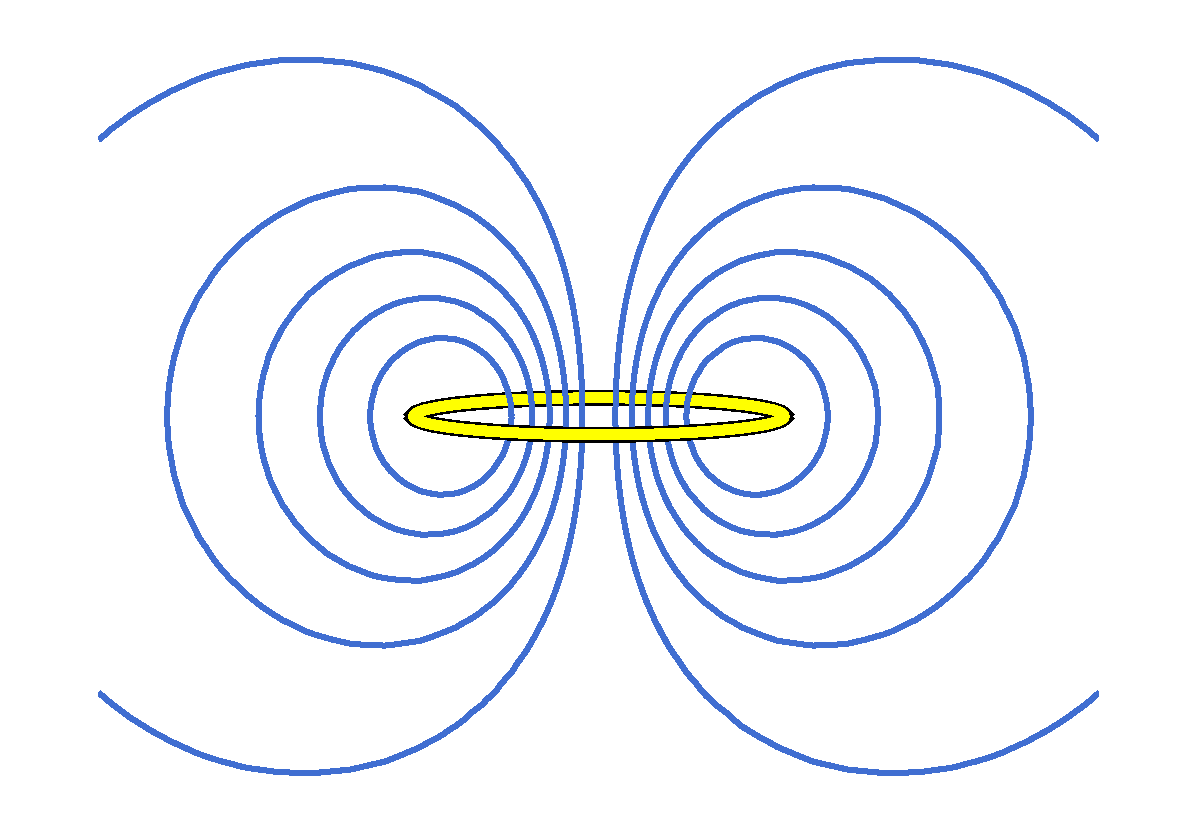
\includegraphics[width=\textwidth]{pic_data/dlhcc.pdf}
\stepcounter{footnote}
\caption{通电圆环磁场\protect \footnotemark[\value{footnote}]}
\end{minipage}
\hfill
\begin{minipage}[b]{0.4\linewidth}
\centering
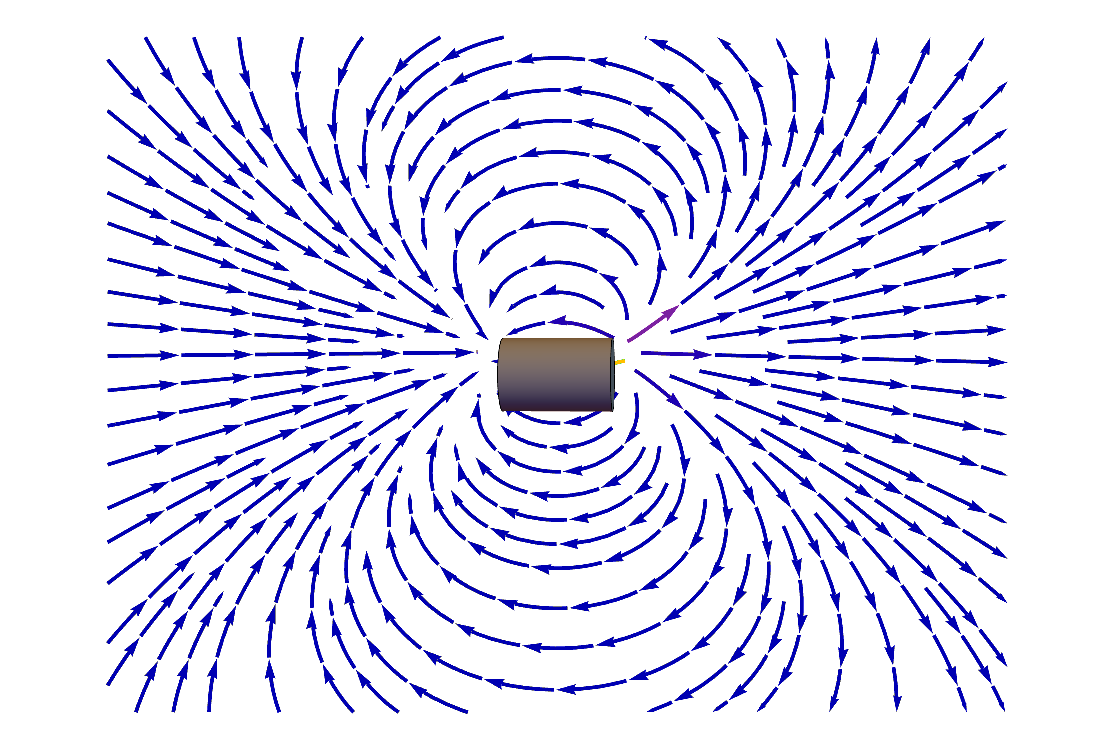
\includegraphics[width=\textwidth]{pic_data/txctcc.pdf}
\stepcounter{footnote}
\caption{条形磁铁磁场\protect \footnotemark[\value{footnote}]}
\end{minipage}
\end{figure}

\addtocounter{footnote}{-1}
\footnotetext[\value{footnote}]{图像原作者:S.M.Blinder 链接:\url{https://demonstrations.wolfram.com/MagneticFieldOfACurrentLoop/},通过CC BY-NC-SA协议共享}
\stepcounter{footnote}
\footnotetext[\value{footnote}]{图像原作者:S.M.Blinder 链接:\url{https://demonstrations.wolfram.com/MagneticFieldOfACylindricalBarMagnet/},通过CC BY-NC-SA协议共享}

%\subsection{}

%# -*- coding: utf-8-unix -*-
%%==================================================
\tikzset{every picture/.style={line width=0.75pt}} %set default line width to 0.75pt    

\chapter{力学}

\section{等时圆}
\begin{center}
\begin{tikzpicture}[x=0.75pt,y=0.75pt,yscale=-1,xscale=1]
%uncomment if require: \path (0,300); %set diagram left start at 0, and has height of 300

%Shape: Circle [id:dp8496772215401891] 
\draw  [dash pattern={on 4.5pt off 4.5pt}] (320,120) .. controls (320,92.39) and (342.39,70) .. (370,70) .. controls (397.61,70) and (420,92.39) .. (420,120) .. controls (420,147.61) and (397.61,170) .. (370,170) .. controls (342.39,170) and (320,147.61) .. (320,120) -- cycle ;
%Straight Lines [id:da857993326744972] 
\draw    (320,120) -- (370,170) ;
%Straight Lines [id:da0897160934147394] 
\draw    (370,170) -- (330,90) ;
%Straight Lines [id:da24569397099487955] 
\draw    (370,170) -- (370,70) ;
%Shape: Circle [id:dp6114455259942786] 
\draw  [dash pattern={on 4.5pt off 4.5pt}] (130,120) .. controls (130,92.39) and (152.39,70) .. (180,70) .. controls (207.61,70) and (230,92.39) .. (230,120) .. controls (230,147.61) and (207.61,170) .. (180,170) .. controls (152.39,170) and (130,147.61) .. (130,120) -- cycle ;
%Straight Lines [id:da5761574734359041] 
\draw    (130,115) -- (180,170) ;
%Straight Lines [id:da11384750291043266] 
\draw  [dash pattern={on 4.5pt off 4.5pt}]  (180,70) -- (130,115) ;
%Straight Lines [id:da2574139608763413] 
\draw  [dash pattern={on 4.5pt off 4.5pt}]  (180,170) -- (180,70) ;
%Straight Lines [id:da5571700478787935] 
\draw    (120,170) -- (240,170) ;
%Straight Lines [id:da6687804622520057] 
\draw    (310,170) -- (430,170) ;

% Text Node
\draw (306,112.4) node [anchor=north west][inner sep=0.75pt]  [font=\tiny]  {$a$};
% Text Node
\draw (321,77.4) node [anchor=north west][inner sep=0.75pt]  [font=\tiny]  {$b$};
% Text Node
\draw (366,57.4) node [anchor=north west][inner sep=0.75pt]  [font=\tiny]  {$c$};
% Text Node
\draw (116,107.4) node [anchor=north west][inner sep=0.75pt]  [font=\tiny]  {$A$};
% Text Node
\draw (156,157.4) node [anchor=north west][inner sep=0.75pt]  [font=\tiny]  {$\theta $};
% Text Node
\draw (176,172.4) node [anchor=north west][inner sep=0.75pt]  [font=\tiny]  {$B$};
% Text Node
\draw (176,57.4) node [anchor=north west][inner sep=0.75pt]  [font=\tiny]  {$C$};
% Text Node
\draw (166,82.4) node [anchor=north west][inner sep=0.75pt]  [font=\tiny]  {$\theta $};


\end{tikzpicture}

\end{center}

如左图,在竖直平面内,有一光滑斜面$AB$,其中$B$点在地面上固定,$A$点可在一圆上运动。设$AB$与地面倾角为$\theta$。由于$A$在圆上,取$C$使得$CB$为直径,则$\angle CAB = 90^{\circ}$,故$\angle ACB = \theta$。记圆的半径为$R$,若有一物体从$A$点下滑至$B$点,则下滑距离$L$为
$$L=2R \sin \theta$$
沿斜面下滑的加速度为
$$a=g \sin \theta$$
故下滑用时为
$$T = \sqrt{\frac{2L}{a}} = \sqrt{\frac{4R}{g}}$$
可以看到下滑时间与$\theta$无关,即右图中物体从$a$、$b$、$c$三个斜面下滑用时相同,我们称图中的圆为“\textbf{等时圆}”。

\begin{theo}{等时圆}{}
物体从圆上任意一点沿斜面无摩擦自由运动到圆上最低点的时间都相等。

同理,物体从圆上最高点沿斜面无摩擦自由运动到圆上任意一点的时间都相等。
\end{theo}

\section{等效重力场}
若物体在空间中运动受到除重力外恒定不变的力,力的大小和方向不随着物体位置的变化而变化(如匀强电场中带电小球所受到的电场力),或者存在恒定不变的加速度(如在加速的电梯中,加速度车厢里),则可以将所受到的恒力产生的加速度或者该恒定不变的加速度的矢量取反后与重力加速度合成成一个新的恒定不变的加速度,即“等效重力加速度”。

\begin{minipage}[b]{0.4\linewidth}
\begin{figure}[H]
\centering
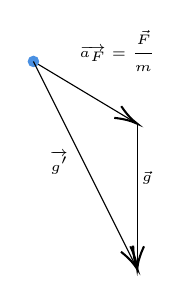
\begin{tikzpicture}[x=0.75pt,y=0.75pt,yscale=-1,xscale=1]
%uncomment if require: \path (0,300); %set diagram left start at 0, and has height of 300

%Straight Lines [id:da6000594042392968] 
\draw    (302.5,70) -- (350.79,98.97) ;
\draw [shift={(352.5,100)}, rotate = 210.96] [color={rgb, 255:red, 0; green, 0; blue, 0 }  ][line width=0.75]    (10.93,-3.29) .. controls (6.95,-1.4) and (3.31,-0.3) .. (0,0) .. controls (3.31,0.3) and (6.95,1.4) .. (10.93,3.29)   ;
%Shape: Circle [id:dp5092551209319207] 
\draw  [color={rgb, 255:red, 74; green, 144; blue, 226 }  ,draw opacity=1 ][fill={rgb, 255:red, 74; green, 144; blue, 226 }  ,fill opacity=1 ] (305,70) .. controls (305,68.62) and (303.88,67.5) .. (302.5,67.5) .. controls (301.12,67.5) and (300,68.62) .. (300,70) .. controls (300,71.38) and (301.12,72.5) .. (302.5,72.5) .. controls (303.88,72.5) and (305,71.38) .. (305,70) -- cycle ;
%Straight Lines [id:da48222497169597345] 
\draw    (352.5,100) -- (352.5,168) ;
\draw [shift={(352.5,170)}, rotate = 270] [color={rgb, 255:red, 0; green, 0; blue, 0 }  ][line width=0.75]    (10.93,-3.29) .. controls (6.95,-1.4) and (3.31,-0.3) .. (0,0) .. controls (3.31,0.3) and (6.95,1.4) .. (10.93,3.29)   ;
%Straight Lines [id:da2944838205191447] 
\draw    (302.5,70) -- (351.61,168.21) ;
\draw [shift={(352.5,170)}, rotate = 243.43] [color={rgb, 255:red, 0; green, 0; blue, 0 }  ][line width=0.75]    (10.93,-3.29) .. controls (6.95,-1.4) and (3.31,-0.3) .. (0,0) .. controls (3.31,0.3) and (6.95,1.4) .. (10.93,3.29)   ;

% Text Node
\draw (323.5,54) node [anchor=north west][inner sep=0.75pt]  [font=\tiny] [align=left] {$\displaystyle \overrightarrow{a_{F}} =\frac{\vec{F}}{m}$};
% Text Node
\draw (353.5,122) node [anchor=north west][inner sep=0.75pt]  [font=\tiny] [align=left] {$\displaystyle \vec{g}$};
% Text Node
\draw (309.5,112) node [anchor=north west][inner sep=0.75pt]  [font=\tiny] [align=left] {$\displaystyle \overrightarrow{g^{\prime }}$};


\end{tikzpicture}

\caption{受到恒力}
\end{figure}
\end{minipage}
\hfill
\begin{minipage}[b]{0.4\linewidth}
\begin{figure}[H]
\centering
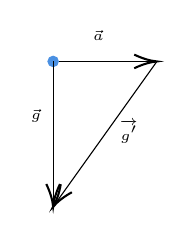
\begin{tikzpicture}[x=0.75pt,y=0.75pt,yscale=-1,xscale=1]
%uncomment if require: \path (0,300); %set diagram left start at 0, and has height of 300

%Straight Lines [id:da6000594042392968] 
\draw    (280,88) -- (328,88) ;
\draw [shift={(330,88)}, rotate = 180] [color={rgb, 255:red, 0; green, 0; blue, 0 }  ][line width=0.75]    (10.93,-3.29) .. controls (6.95,-1.4) and (3.31,-0.3) .. (0,0) .. controls (3.31,0.3) and (6.95,1.4) .. (10.93,3.29)   ;
%Shape: Circle [id:dp5092551209319207] 
\draw  [color={rgb, 255:red, 74; green, 144; blue, 226 }  ,draw opacity=1 ][fill={rgb, 255:red, 74; green, 144; blue, 226 }  ,fill opacity=1 ] (282.5,88) .. controls (282.5,86.62) and (281.38,85.5) .. (280,85.5) .. controls (278.62,85.5) and (277.5,86.62) .. (277.5,88) .. controls (277.5,89.38) and (278.62,90.5) .. (280,90.5) .. controls (281.38,90.5) and (282.5,89.38) .. (282.5,88) -- cycle ;
%Straight Lines [id:da48222497169597345] 
\draw    (280,88) -- (280,156) ;
\draw [shift={(280,158)}, rotate = 270] [color={rgb, 255:red, 0; green, 0; blue, 0 }  ][line width=0.75]    (10.93,-3.29) .. controls (6.95,-1.4) and (3.31,-0.3) .. (0,0) .. controls (3.31,0.3) and (6.95,1.4) .. (10.93,3.29)   ;
%Straight Lines [id:da2944838205191447] 
\draw    (330,88) -- (281.16,156.37) ;
\draw [shift={(280,158)}, rotate = 305.54] [color={rgb, 255:red, 0; green, 0; blue, 0 }  ][line width=0.75]    (10.93,-3.29) .. controls (6.95,-1.4) and (3.31,-0.3) .. (0,0) .. controls (3.31,0.3) and (6.95,1.4) .. (10.93,3.29)   ;

% Text Node
\draw (298,72) node [anchor=north west][inner sep=0.75pt]  [font=\tiny] [align=left] {$\displaystyle \vec{a}$};
% Text Node
\draw (268,110) node [anchor=north west][inner sep=0.75pt]  [font=\tiny] [align=left] {$\displaystyle \vec{g}$};
% Text Node
\draw (311,115) node [anchor=north west][inner sep=0.75pt]  [font=\tiny] [align=left] {$\displaystyle \overrightarrow{g^{\prime }}$};


\end{tikzpicture}
    \caption{存在恒加速}
\end{figure}
\end{minipage}
~\\
右图涉及到换系下加速度牵连,可参考\secref{s_sdql},图中$\vec{a}$为绝对加速度,$\vec{g^{\prime}}$为牵连加速度,$\vec{g}$为相对加速度。
\begin{defi}{等效重力加速度}{}

(1)若物体受到除重力外恒力$\vec{F}$,其对物体产生的加速度为$\vec{a_F} = \frac{\vec{F}}{m}$,则等效重力加速度为$\vec{g^{\prime}} = \vec{g} + \vec{a_F}$

(2)若物体在地面系中存在恒定不变的加速度$\vec{a}$,则在一同相对地面加速的参考系中,等效重力加速度\footnote{此处为负号的原因可参考\secref{s_gxl},相当于将加速度等效成惯性力后转化为力平衡问题}为$\vec{g^{\prime}} = \vec{g} - \vec{a}$
\end{defi}

引入等效重力场,我们便可以将一个复合场问题转化为一个单场问题从而运用重力场中运动的结论,或者将一个存在加速的动力学问题转化为一个静力学问题从而进行受力分析,简化解题过程。

\begin{ep}{2017·上海}{}
一碗水置于火车车厢内的水平桌面上。当火车向右做匀减速运动时,水面形状接近于图()
\begin{center}

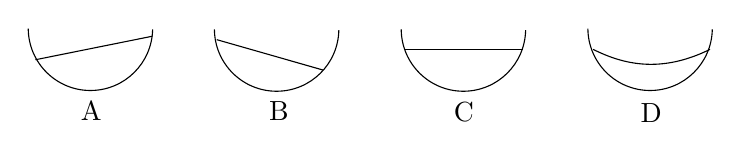
\begin{tikzpicture}[x=0.75pt,y=0.75pt,yscale=-1,xscale=1]
%uncomment if require: \path (0,300); %set diagram left start at 0, and has height of 300

%Shape: Arc [id:dp02201782323269219] 
\draw  [draw opacity=0] (200.11,80.41) .. controls (199.8,96.63) and (186.62,109.72) .. (170.33,109.82) .. controls (153.78,109.92) and (140.28,96.57) .. (140.18,80) -- (170.15,79.82) -- cycle ; \draw   (200.11,80.41) .. controls (199.8,96.63) and (186.62,109.72) .. (170.33,109.82) .. controls (153.78,109.92) and (140.28,96.57) .. (140.18,80) ;  
%Shape: Arc [id:dp6725595721077255] 
\draw  [draw opacity=0] (289.82,80.77) .. controls (289.51,96.99) and (276.33,110.08) .. (260.03,110.18) .. controls (243.48,110.28) and (229.98,96.93) .. (229.88,80.36) -- (259.85,80.18) -- cycle ; \draw   (289.82,80.77) .. controls (289.51,96.99) and (276.33,110.08) .. (260.03,110.18) .. controls (243.48,110.28) and (229.98,96.93) .. (229.88,80.36) ;  
%Shape: Arc [id:dp9874905979681834] 
\draw  [draw opacity=0] (379.82,80.77) .. controls (379.51,96.99) and (366.33,110.08) .. (350.03,110.18) .. controls (333.48,110.28) and (319.98,96.93) .. (319.88,80.36) -- (349.85,80.18) -- cycle ; \draw   (379.82,80.77) .. controls (379.51,96.99) and (366.33,110.08) .. (350.03,110.18) .. controls (333.48,110.28) and (319.98,96.93) .. (319.88,80.36) ;  
%Shape: Arc [id:dp48856074542208816] 
\draw  [draw opacity=0] (469.76,80.41) .. controls (469.44,96.63) and (456.26,109.73) .. (439.97,109.82) .. controls (423.42,109.92) and (409.92,96.57) .. (409.82,80.01) -- (439.79,79.82) -- cycle ; \draw   (469.76,80.41) .. controls (469.44,96.63) and (456.26,109.73) .. (439.97,109.82) .. controls (423.42,109.92) and (409.92,96.57) .. (409.82,80.01) ;  
%Straight Lines [id:da697877989538783] 
\draw    (143.67,95) -- (200,83.67) ;
%Straight Lines [id:da3937973345184078] 
\draw    (231,85.33) -- (282.33,100) ;
%Straight Lines [id:da2517825105670837] 
\draw    (321.67,90) -- (378.33,90) ;
%Curve Lines [id:da8533563240632736] 
\draw    (412.33,90) .. controls (427,97.33) and (445,101.67) .. (468.67,90) ;

% Text Node
\draw (164.33,114) node [anchor=north west][inner sep=0.75pt]   [align=left] {A};
% Text Node
\draw (255,114) node [anchor=north west][inner sep=0.75pt]   [align=left] {B};
% Text Node
\draw (344,114.33) node [anchor=north west][inner sep=0.75pt]   [align=left] {C};
% Text Node
\draw (434,115) node [anchor=north west][inner sep=0.75pt]   [align=left] {D};


\end{tikzpicture}

\end{center}
\begin{minipage}[b]{0.6\linewidth}
由于火车向右减速运动,故存在向左的加速度,在火车参考系中等效重力加速度如图所示,由于液面与等效重力加速度垂直(参考现实中水面),故液面应如图中虚线所示,故答案选A
\end{minipage}
\hfill
\begin{minipage}[b]{0.3\linewidth}
\begin{center}

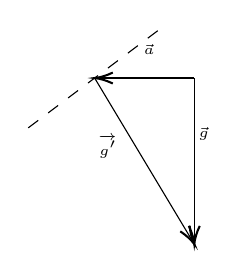
\begin{tikzpicture}[x=0.75pt,y=0.75pt,yscale=-0.8,xscale=0.8]
%uncomment if require: \path (0,300); %set diagram left start at 0, and has height of 300

%Straight Lines [id:da05270942730125916] 
\draw    (320,80) -- (262,80) ;
\draw [shift={(260,80)}, rotate = 360] [color={rgb, 255:red, 0; green, 0; blue, 0 }  ][line width=0.75]    (10.93,-3.29) .. controls (6.95,-1.4) and (3.31,-0.3) .. (0,0) .. controls (3.31,0.3) and (6.95,1.4) .. (10.93,3.29)   ;
%Straight Lines [id:da7697982364741902] 
\draw    (320,80) -- (320,178) ;
\draw [shift={(320,180)}, rotate = 270] [color={rgb, 255:red, 0; green, 0; blue, 0 }  ][line width=0.75]    (10.93,-3.29) .. controls (6.95,-1.4) and (3.31,-0.3) .. (0,0) .. controls (3.31,0.3) and (6.95,1.4) .. (10.93,3.29)   ;
%Straight Lines [id:da5282396830046765] 
\draw    (260,80) -- (318.97,178.29) ;
\draw [shift={(320,180)}, rotate = 239.04] [color={rgb, 255:red, 0; green, 0; blue, 0 }  ][line width=0.75]    (10.93,-3.29) .. controls (6.95,-1.4) and (3.31,-0.3) .. (0,0) .. controls (3.31,0.3) and (6.95,1.4) .. (10.93,3.29)   ;
%Straight Lines [id:da7008344676875142] 
\draw  [dash pattern={on 4.5pt off 4.5pt}]  (220,110) -- (300,50) ;

% Text Node
\draw (288,58) node [anchor=north west][inner sep=0.75pt]  [font=\tiny] [align=left] {$\displaystyle \vec{a}$};
% Text Node
\draw (261,113) node [anchor=north west][inner sep=0.75pt]  [font=\tiny] [align=left] {$\displaystyle \overrightarrow{g^{\prime }}$};
% Text Node
\draw (321,108) node [anchor=north west][inner sep=0.75pt]  [font=\tiny] [align=left] {$\displaystyle \vec{g}$};


\end{tikzpicture}

\end{center}
\end{minipage}
\end{ep}

\begin{ep}{2015·海南}{}
如图所示,升降机内有固定斜面,斜面上放物块。开始时,升降机做匀速运动,物块相对于斜面匀速下滑。当升降机加速上升时()

\begin{minipage}[b]{0.6\linewidth}
\begin{enumerate}[label=(\Alph*)]
  \item 物块与斜面间的摩擦力减小
  \item 物块与斜面间的正压力增大
  \item 物块相对于斜面减速下滑
  \item 物块相对于斜面匀速下滑
\end{enumerate}
\end{minipage}
\hfill
\begin{minipage}[b]{0.3\linewidth}
\begin{center}

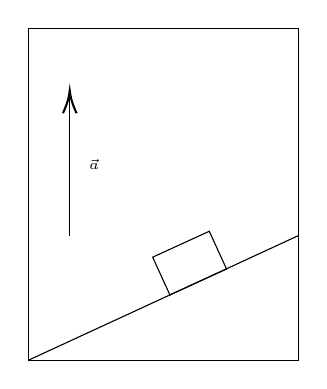
\begin{tikzpicture}[x=0.75pt,y=0.75pt,yscale=-1,xscale=1]
%uncomment if require: \path (0,300); %set diagram left start at 0, and has height of 300

%Shape: Rectangle [id:dp12246987109761442] 
\draw   (200,40) -- (330,40) -- (330,200) -- (200,200) -- cycle ;
%Straight Lines [id:da9008116307778782] 
\draw    (200,200) -- (330,140) ;
%Shape: Rectangle [id:dp03770706202210139] 
\draw   (259.95,150.31) -- (287.23,137.83) -- (295.55,156.02) -- (268.26,168.5) -- cycle ;
%Straight Lines [id:da8731919724345383] 
\draw    (220,140) -- (220,72) ;
\draw [shift={(220,70)}, rotate = 90] [color={rgb, 255:red, 0; green, 0; blue, 0 }  ][line width=0.75]    (10.93,-3.29) .. controls (6.95,-1.4) and (3.31,-0.3) .. (0,0) .. controls (3.31,0.3) and (6.95,1.4) .. (10.93,3.29)   ;

% Text Node
\draw (228,102) node [anchor=north west][inner sep=0.75pt]  [font=\tiny] [align=left] {$\displaystyle \vec{a}$};


\end{tikzpicture}

\end{center}
\end{minipage}
~\\

\begin{minipage}[b]{0.6\linewidth}
~\\

对物块受力分析,升降机匀速时,列受力平衡:
$$N = mg \cos{\theta} ,\quad f=\mu N = mg \sin{\theta}$$
故解得匀速条件$\mu = \tan{\theta}$。

当升降机以加速度$a$上升时,以升降机为参考系,等效重力加速度$g^{\prime}=g+a$,将$g^{\prime}$替换上式$g$,得到$N$增大,$f$增大,由于前文解出匀速运动条件$\mu = \tan{\theta}$与$g$无关,则升降机加速后仍旧保持匀速运动,故选BD。

\end{minipage}
\hfill
\begin{minipage}[b]{0.3\linewidth}
\begin{center}

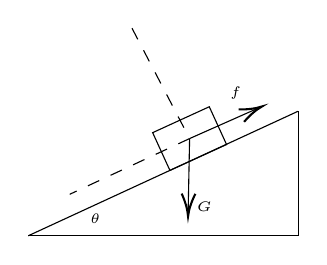
\begin{tikzpicture}[x=0.75pt,y=0.75pt,yscale=-1,xscale=1]
%uncomment if require: \path (0,300); %set diagram left start at 0, and has height of 300

%Straight Lines [id:da9008116307778782] 
\draw    (200,200) -- (330,140) ;
%Shape: Rectangle [id:dp03770706202210139] 
\draw   (259.95,150.31) -- (287.23,137.83) -- (295.55,156.02) -- (268.26,168.5) -- cycle ;
%Straight Lines [id:da8341542863429008] 
\draw    (200,200) -- (330,200) ;
%Straight Lines [id:da1419286936694566] 
\draw    (330,140) -- (330,200) ;
%Straight Lines [id:da8505072201094237] 
\draw  [dash pattern={on 4.5pt off 4.5pt}]  (277.75,153.16) -- (220,180) ;
%Straight Lines [id:da9138661314002989] 
\draw  [dash pattern={on 4.5pt off 4.5pt}]  (250,100) -- (277.75,153.16) ;
%Straight Lines [id:da2057884653890707] 
\draw    (277.75,153.16) -- (277.04,188.67) ;
\draw [shift={(277,190.67)}, rotate = 271.14] [color={rgb, 255:red, 0; green, 0; blue, 0 }  ][line width=0.75]    (10.93,-3.29) .. controls (6.95,-1.4) and (3.31,-0.3) .. (0,0) .. controls (3.31,0.3) and (6.95,1.4) .. (10.93,3.29)   ;
%Straight Lines [id:da1801333502686453] 
\draw    (277.75,153.16) -- (310.84,138.48) ;
\draw [shift={(312.67,137.67)}, rotate = 156.07] [color={rgb, 255:red, 0; green, 0; blue, 0 }  ][line width=0.75]    (10.93,-3.29) .. controls (6.95,-1.4) and (3.31,-0.3) .. (0,0) .. controls (3.31,0.3) and (6.95,1.4) .. (10.93,3.29)   ;

% Text Node
\draw (280,182.33) node [anchor=north west][inner sep=0.75pt]  [font=\tiny] [align=left] {$\displaystyle G$};
% Text Node
\draw (296,127) node [anchor=north west][inner sep=0.75pt]  [font=\tiny] [align=left] {$\displaystyle f$};
% Text Node
\draw (228.67,188) node [anchor=north west][inner sep=0.75pt]  [font=\tiny] [align=left] {$\displaystyle \theta $};


\end{tikzpicture}

\end{center}
\end{minipage}

\end{ep}
\section{类平抛与偏转角关系}

若物体在空间中运动受到恒定不变的力,且该物体的初速度方向与所受力的方向垂直,则该物体做类平抛运动(当只受重力作用时,便为经典的平抛运动),以运动初速度方向为x轴,受力方向为y轴,建系。设运动初速度为$v_x$,运动时间为$t$,加速度$a = \frac{F}{m}$,则有
\begin{equation}
\begin{aligned}
x &= v_x t \\
y &= \frac{1}{2} a t^2 \\
v_y &= a t
\end{aligned}
\label{e_lpp1}
\end{equation}

记速度偏向角为$\theta_v$,位移偏向角为$\theta_r$,则有

\begin{center}

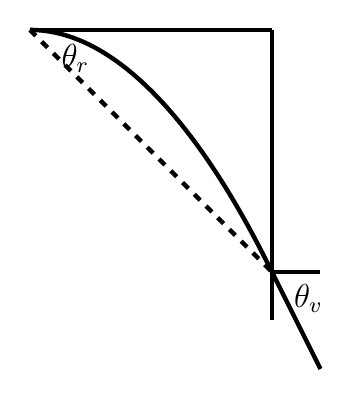
\begin{tikzpicture}[x=35pt,y=35pt,yscale=0.5,xscale=0.5]
\draw [ultra thick] (0,0) parabola (5,-5); % 默认以起始点为极值点
\draw [ultra thick] (0,0) -- (5,0);
\draw [ultra thick] (5,0) -- (5,-6);
\draw [dashed,ultra thick] (0,0) -- (5,-5);
\draw [ultra thick] (5,-5) -- (6,-7);
\draw [ultra thick] (5,-5) -- (6,-5);
\draw (0.6,-0.25) node [anchor=north west][inner sep=0.75pt][font=\large][align=left] {$\theta_{r}$};
\draw (5.4,-5.2) node [anchor=north west][inner sep=0.75pt][font=\large][align=left] {$\theta_{v}$};
\end{tikzpicture}

\end{center}

\begin{equation}
\tan{\theta_v} = \frac{v_y}{v_x} ,\quad \tan{\theta_r} = \frac{y}{x}
\label{e_sdwypxj}
\end{equation}

将式\eqref{e_lpp1}带入式\eqref{e_sdwypxj},解得

\begin{equation}
\boxed{\tan{\theta_v} = 2 \tan{\theta_r}}
\end{equation}

\begin{theo}{类平抛速度偏向角与位移偏向角关系}{}
在类平抛运动中,记速度偏向角为$\theta_v$,位移偏向角为$\theta_r$,则有

$$\tan{\theta_v} = 2 \tan{\theta_r}$$

即\textbf{速度偏向角正切值等于位移偏向角正切值二倍}。
\end{theo}

此定理可以在求解类平抛运动的问题中简化计算。如知道位移偏转角马上便可求出速度偏转角,跳过联立求解的步骤,进而求出速度改变量,进一步求出运动时间等其他参量。

\begin{ep}{练习题}{}
如图所示,斜面固定在水平面上,两个小球分别从0点正上方A、B两点向右水平抛出,B为AO连线的中点,最后两球都垂直落在斜面上,A、B两球击中斜面位置到0点的距离比为()

\begin{minipage}[b]{0.6\linewidth}
\begin{enumerate}[label=(\Alph*)]
  \item $\sqrt{2}:1$
  \item $2:1$
  \item $4:\sqrt{2}$
  \item $4:1$
\end{enumerate}
\end{minipage}
\hfill
\begin{minipage}[b]{0.3\linewidth}
\begin{center}

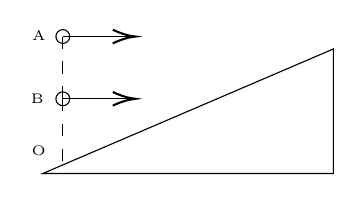
\begin{tikzpicture}[x=0.75pt,y=0.75pt,yscale=-1,xscale=1]
%uncomment if require: \path (0,300); %set diagram left start at 0, and has height of 300

%Shape: Right Triangle [id:dp5854952839998064] 
\draw   (220,160) -- (80,220) -- (220,220) -- cycle ;
%Shape: Circle [id:dp2853490737518214] 
\draw   (86.33,184) .. controls (86.33,182.16) and (87.83,180.67) .. (89.67,180.67) .. controls (91.51,180.67) and (93,182.16) .. (93,184) .. controls (93,185.84) and (91.51,187.33) .. (89.67,187.33) .. controls (87.83,187.33) and (86.33,185.84) .. (86.33,184) -- cycle ;
%Shape: Circle [id:dp04536789699196353] 
\draw   (86.33,154) .. controls (86.33,152.16) and (87.83,150.67) .. (89.67,150.67) .. controls (91.51,150.67) and (93,152.16) .. (93,154) .. controls (93,155.84) and (91.51,157.33) .. (89.67,157.33) .. controls (87.83,157.33) and (86.33,155.84) .. (86.33,154) -- cycle ;
%Straight Lines [id:da7954201931557305] 
\draw    (89.67,184) -- (122.67,184) ;
\draw [shift={(124.67,184)}, rotate = 180] [color={rgb, 255:red, 0; green, 0; blue, 0 }  ][line width=0.75]    (10.93,-3.29) .. controls (6.95,-1.4) and (3.31,-0.3) .. (0,0) .. controls (3.31,0.3) and (6.95,1.4) .. (10.93,3.29)   ;
%Straight Lines [id:da8343490951051455] 
\draw    (89.67,154) -- (122.67,154) ;
\draw [shift={(124.67,154)}, rotate = 180] [color={rgb, 255:red, 0; green, 0; blue, 0 }  ][line width=0.75]    (10.93,-3.29) .. controls (6.95,-1.4) and (3.31,-0.3) .. (0,0) .. controls (3.31,0.3) and (6.95,1.4) .. (10.93,3.29)   ;
%Straight Lines [id:da8916316090315564] 
\draw  [dash pattern={on 4.5pt off 4.5pt}]  (89.67,154) -- (89.67,184) ;
%Straight Lines [id:da34383387037199364] 
\draw  [dash pattern={on 4.5pt off 4.5pt}]  (89.67,184) -- (89.67,214) ;

% Text Node
\draw (73,180.33) node [anchor=north west][inner sep=0.75pt]  [font=\tiny] [align=left] {B};
% Text Node
\draw (73.67,150) node [anchor=north west][inner sep=0.75pt]  [font=\tiny] [align=left] {A};
% Text Node
\draw (73.33,205.67) node [anchor=north west][inner sep=0.75pt]  [font=\tiny] [align=left] {O};


\end{tikzpicture}


\end{center}
\end{minipage}
~\\

由题可知,最后两球都垂直落在斜面上,两球速度偏转角$\theta_v$相同,故两球位移偏转角$\theta_r$相同,故两球落点距O点距离与AO和BO成比例,即2:1,故选B。
\end{ep}

\section{摩擦角与全反力}

若一物体放在粗糙水平面上,物体与水平面间摩擦系数为$\mu$,设水平面给该物体的支持力为$N$。若该物体\textbf{相对水平面发生滑动},则该物体受到的滑动摩擦为$\mu N$。

\begin{center}
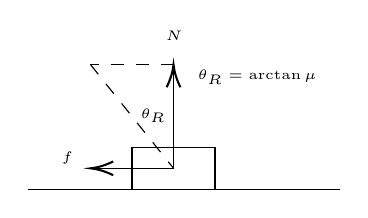
\begin{tikzpicture}[x=0.75pt,y=0.75pt,yscale=-1,xscale=1]
%uncomment if require: \path (0,300); %set diagram left start at 0, and has height of 300

%Straight Lines [id:da524357483065941] 
\draw    (140,130) -- (290,130) ;
%Shape: Rectangle [id:dp1562964743350983] 
\draw   (190,110) -- (230,110) -- (230,130) -- (190,130) -- cycle ;
%Straight Lines [id:da659959210580102] 
\draw    (210,120) -- (210,72) ;
\draw [shift={(210,70)}, rotate = 90] [color={rgb, 255:red, 0; green, 0; blue, 0 }  ][line width=0.75]    (10.93,-3.29) .. controls (6.95,-1.4) and (3.31,-0.3) .. (0,0) .. controls (3.31,0.3) and (6.95,1.4) .. (10.93,3.29)   ;
%Straight Lines [id:da5537782404532552] 
\draw    (210,120) -- (172,120) ;
\draw [shift={(170,120)}, rotate = 360] [color={rgb, 255:red, 0; green, 0; blue, 0 }  ][line width=0.75]    (10.93,-3.29) .. controls (6.95,-1.4) and (3.31,-0.3) .. (0,0) .. controls (3.31,0.3) and (6.95,1.4) .. (10.93,3.29)   ;
%Straight Lines [id:da5271088999254347] 
\draw  [dash pattern={on 4.5pt off 4.5pt}]  (210,70) -- (170,70) ;
%Straight Lines [id:da223898729028551] 
\draw  [dash pattern={on 4.5pt off 4.5pt}]  (170,70) -- (210,120) ;

% Text Node
\draw (155,111) node [anchor=north west][inner sep=0.75pt]  [font=\tiny] [align=left] {$\displaystyle f$};
% Text Node
\draw (205,52.5) node [anchor=north west][inner sep=0.75pt]  [font=\tiny] [align=left] {$\displaystyle N$};
% Text Node
\draw (193,90) node [anchor=north west][inner sep=0.75pt]  [font=\tiny] [align=left] {$\displaystyle \theta_R $};
% Text Node
\draw (220.5,71.5) node [anchor=north west][inner sep=0.75pt]  [font=\tiny] [align=left] {$\displaystyle \theta_R =\arctan \mu $};


\end{tikzpicture}

\end{center}

\begin{defi}{摩擦角和全反力}{}
如图所示,现在我们将该物体受到的\textbf{支持力}与\textbf{摩擦力}等效为一个力,我们称支持力与摩擦力的合力为\textbf{全反力},记为$R$。由图可见,\textbf{若物体与地面发生相对滑动},则全反力的方向固定,记$\theta_R$为全反力与竖直方向夹角。则

$$\tan{\theta_R}  = \frac{\mu N}{N} = \mu$$

即\textbf{摩擦角的正切值等于摩擦系数}。
\end{defi}

巧妙运用全反力,可以将\textbf{四力平衡简化为三力平衡},从而\textbf{运用力的矢量三角形}分析问题,从而简化分析计算。具体操作见如下例题

\begin{ep}{练习题}{}
如图,水平地面上有一木箱,木箱与地面间的动摩擦因数为$\mu$。现对木箱施加一拉力$F$,使木箱做匀速直线运动。设$F$的方向与水平地面的夹角为$\alpha$,在$\theta$从$0^{\circ}$逐渐增大到$90^{\circ}$的过程中,木箱的速度保持不变,则()


\begin{minipage}[b]{0.6\linewidth}
(A) $F$先减小后增大 \quad (B) $F$一直增大

(C) $F$先增大后减小 \quad (D) $F$一直减小
\end{minipage}
\hfill
\begin{minipage}[b]{0.3\linewidth}
\begin{center}
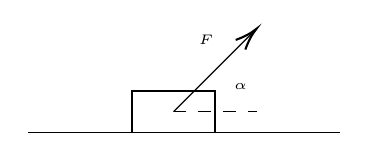
\begin{tikzpicture}[x=0.75pt,y=0.75pt,yscale=-1,xscale=1]
%uncomment if require: \path (0,300); %set diagram left start at 0, and has height of 300

%Straight Lines [id:da945561223656612] 
\draw    (160,150) -- (310,150) ;
%Shape: Rectangle [id:dp34505167057606223] 
\draw   (210,130) -- (250,130) -- (250,150) -- (210,150) -- cycle ;
%Straight Lines [id:da9917012861214194] 
\draw    (230,140) -- (268.59,101.41) ;
\draw [shift={(270,100)}, rotate = 135] [color={rgb, 255:red, 0; green, 0; blue, 0 }  ][line width=0.75]    (10.93,-3.29) .. controls (6.95,-1.4) and (3.31,-0.3) .. (0,0) .. controls (3.31,0.3) and (6.95,1.4) .. (10.93,3.29)   ;
%Straight Lines [id:da49493046166366783] 
\draw  [dash pattern={on 4.5pt off 4.5pt}]  (230,140) -- (270,140) ;

% Text Node
\draw (258,125) node [anchor=north west][inner sep=0.75pt]  [font=\tiny] [align=left] {$\displaystyle \alpha $};
% Text Node
\draw (241,102) node [anchor=north west][inner sep=0.75pt]  [font=\tiny] [align=left] {$\displaystyle F$};


\end{tikzpicture}

\end{center}
\end{minipage}
~\\

\begin{minipage}[b]{0.6\linewidth}
由于木箱速度保持恒定不变,故木箱一直受力平衡。由前文知,摩擦力$f$与压力$N$的合力全反力$R$方向恒定,沿图中虚线方向。
\end{minipage}
\hfill
\begin{minipage}[b]{0.3\linewidth}
\begin{center}
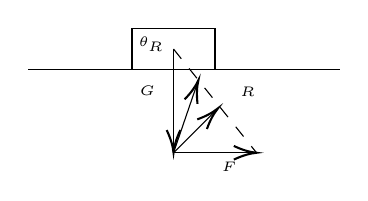
\begin{tikzpicture}[x=0.75pt,y=0.75pt,yscale=-1,xscale=1]
%uncomment if require: \path (0,300); %set diagram left start at 0, and has height of 300

%Straight Lines [id:da524357483065941] 
\draw    (140,130) -- (290,130) ;
%Shape: Rectangle [id:dp1562964743350983] 
\draw   (190,110) -- (230,110) -- (230,130) -- (190,130) -- cycle ;
%Straight Lines [id:da659959210580102] 
\draw    (210,120) -- (210,168) ;
\draw [shift={(210,170)}, rotate = 270] [color={rgb, 255:red, 0; green, 0; blue, 0 }  ][line width=0.75]    (10.93,-3.29) .. controls (6.95,-1.4) and (3.31,-0.3) .. (0,0) .. controls (3.31,0.3) and (6.95,1.4) .. (10.93,3.29)   ;
%Straight Lines [id:da223898729028551] 
\draw  [dash pattern={on 4.5pt off 4.5pt}]  (210,120) -- (250,170) ;
%Straight Lines [id:da7461771596827373] 
\draw    (210,170) -- (248,170) ;
\draw [shift={(250,170)}, rotate = 180] [color={rgb, 255:red, 0; green, 0; blue, 0 }  ][line width=0.75]    (10.93,-3.29) .. controls (6.95,-1.4) and (3.31,-0.3) .. (0,0) .. controls (3.31,0.3) and (6.95,1.4) .. (10.93,3.29)   ;
%Straight Lines [id:da7253181021320425] 
\draw    (210,170) -- (230.09,149.91) ;
\draw [shift={(231.5,148.5)}, rotate = 135] [color={rgb, 255:red, 0; green, 0; blue, 0 }  ][line width=0.75]    (10.93,-3.29) .. controls (6.95,-1.4) and (3.31,-0.3) .. (0,0) .. controls (3.31,0.3) and (6.95,1.4) .. (10.93,3.29)   ;
%Straight Lines [id:da030028220247521498] 
\draw    (210,170) -- (221.35,136.89) ;
\draw [shift={(222,135)}, rotate = 108.92] [color={rgb, 255:red, 0; green, 0; blue, 0 }  ][line width=0.75]    (10.93,-3.29) .. controls (6.95,-1.4) and (3.31,-0.3) .. (0,0) .. controls (3.31,0.3) and (6.95,1.4) .. (10.93,3.29)   ;

% Text Node
\draw (192,113) node [anchor=north west][inner sep=0.75pt]  [font=\tiny] [align=left] {$\displaystyle \theta _{R}$};
% Text Node
\draw (192.5,136.5) node [anchor=north west][inner sep=0.75pt]  [font=\tiny] [align=left] {$\displaystyle G$};
% Text Node
\draw (232,173) node [anchor=north west][inner sep=0.75pt]  [font=\tiny] [align=left] {$\displaystyle F$};
% Text Node
\draw (236.5,138) node [anchor=north west][inner sep=0.75pt]  [font=\tiny] [align=left] {$ $};
% Text Node
\draw (241,137) node [anchor=north west][inner sep=0.75pt]  [font=\tiny] [align=left] {$\displaystyle R$};


\end{tikzpicture}

\end{center}
\end{minipage}

由于木箱受力平衡,故全反力$R$(替代了摩擦力$f$与压力$N$),重力$G$,拉力$F$三力平衡,原本四力平衡问题化为三力平衡问题。由力的矢量三角形知,拉力$F$先减小,再增大,故选A。
\end{ep}

\begin{mk}{思考}{}
设上题木块质量为$m$,试用摩擦角和全反力求出$F$的最小值$F_{min}$和此时与地面夹角$\alpha$。
\end{mk}

\section{整体牛二定律}

对于一个系统,若该系统由$n$个质点构成,外界对物体有力的作用(外力),质点之间也有力的作用(内力),记第$i$个质点的质量为$m_i$,加速度为$\vec{a_i}$,作用在第$i$个质点的外力为$\vec{F_i}$,第$i$个质点对第$j$个质点的内力为$\vec{f_{ij}}$,则
\begin{subequations}
\begin{align*}
\vec{F_1} + \sum_{i=1}^{n} \vec{f_{i1}} &= m_1 \vec{a_1} \\
\vec{F_2} + \sum_{i=1}^{n} \vec{f_{i2}} &= m_2 \vec{a_2} \\
&\vdots \\
\vec{F_n} + \sum_{i=1}^{n} \vec{f_{in}} &= m_n \vec{a_n} 
\end{align*}
\end{subequations}

注意到$\vec{f_{ij}} = - \vec{f_{ji}}$,$\vec{f_{ii}}=\vec{0}$对等式两边求和,得

$$\vec{F} = \sum \vec{F_i} = \sum m_i \vec{a_i}$$

\begin{theo}{整体牛二定律}{}
对于一个多质点系统,其所受合外力与各质点加速度满足

$$\vec{F} = \sum \vec{F_i} = \sum m_i \vec{a_i}$$

其中第$i$个质点的质量为$m_i$,加速度为$\vec{a_i}$。
\end{theo}

整体牛二定律可以帮助我们跳过繁琐的内力求解,运用整体法直接求出系统所受外力。具体见如下例题

\begin{ep}{练习题}{}
\begin{minipage}[b]{0.6\linewidth}
一个箱子放在水平地面上,箱内有一固定的竖直杆,在杆上套着一个环,箱与杆的质量为$M$,环的质量为$m$。如图所示。已知环沿杆以加速度$a$匀加速下滑,则此时箱对地面的压力大小为()

(A) $Mg-ma$ \quad (B) $Mg$

(C) $Mg+mg$ \quad (D) $Mg+mg-ma$
\end{minipage}
\hfill
\begin{minipage}[b]{0.3\linewidth}
\begin{center}

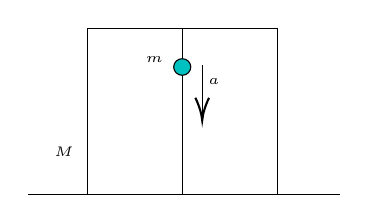
\begin{tikzpicture}[x=0.75pt,y=0.75pt,yscale=-1,xscale=1]
%uncomment if require: \path (0,300); %set diagram left start at 0, and has height of 300

%Shape: Rectangle [id:dp9922461305951003] 
\draw   (178.4,60) -- (270,60) -- (270,140) -- (178.4,140) -- cycle ;
%Straight Lines [id:da3301501137208056] 
\draw    (224.2,60) -- (224.2,140) ;
%Shape: Ellipse [id:dp5458618741603067] 
\draw  [color={rgb, 255:red, 0; green, 0; blue, 0 }  ,draw opacity=1 ][fill={rgb, 255:red, 0; green, 192; blue, 192 }  ,fill opacity=1 ] (220.08,78.67) .. controls (220.08,76.46) and (221.93,74.67) .. (224.2,74.67) .. controls (226.48,74.67) and (228.32,76.46) .. (228.32,78.67) .. controls (228.32,80.88) and (226.48,82.67) .. (224.2,82.67) .. controls (221.93,82.67) and (220.08,80.88) .. (220.08,78.67) -- cycle ;
%Straight Lines [id:da7738101207130361] 
\draw    (233.82,77.78) -- (233.82,102.44) ;
\draw [shift={(233.82,104.44)}, rotate = 270] [color={rgb, 255:red, 0; green, 0; blue, 0 }  ][line width=0.75]    (10.93,-3.29) .. controls (6.95,-1.4) and (3.31,-0.3) .. (0,0) .. controls (3.31,0.3) and (6.95,1.4) .. (10.93,3.29)   ;
%Straight Lines [id:da09431715141860386] 
\draw    (150,140) -- (300,140) ;

% Text Node
\draw (161.37,116.17) node [anchor=north west][inner sep=0.75pt]  [font=\tiny] [align=left] {$\displaystyle M$};
% Text Node
\draw (205.42,72.61) node [anchor=north west][inner sep=0.75pt]  [font=\tiny] [align=left] {$\displaystyle m$};
% Text Node
\draw (235.65,82.83) node [anchor=north west][inner sep=0.75pt]  [font=\tiny] [align=left] {$\displaystyle a$};


\end{tikzpicture}

\end{center}
\end{minipage}
~\\

取整体为研究对象,箱加速度为$0$,环加速度为$a$,设$N$为箱对地面压力,对整体列整体牛二方程,得
$$Mg+mg-N=0 + ma$$
解得$N=Mg+mg-ma$,故选D。
\end{ep}

\section{图解旋转弹簧类问题}

对于弹簧,有胡克定律$F=kx$,其中$x$为弹簧形变量,可以看到弹力与弹簧形变量成正比,故如果我们能用图示表示出弹簧形变量,我们便可以半定量地画出弹力的大小和方向,从而便于我们运用力的矢量三角形分析其他力的变化。

一个基本想法是,找到弹簧处于原长时候的位置,以旋转弹簧定点为圆心,原长为半径,画圆。当弹簧不在原长时,作弹簧所在直线,交圆于一点,\textbf{该点与弹簧动点距离即表征弹力大小}。具体操作参考下面例题。

\begin{ep}{练习题}{}
如图所示,A、B两物块始终静止在水平地面上,一轻质弹簧一端连接在竖直墙上P点,另一端与A相连接,下列说法正确的是()

\begin{minipage}[b]{0.6\linewidth}
\begin{enumerate}[label=(\Alph*)]
  \item 如果B对A无摩擦力,则地面对B也无摩擦力
  \item 如果B对A有向左的摩擦力,则地面对B也有向左的摩擦力
  \item P点缓慢下移过程中,B对A的支持力一定减小
  \item P点缓慢下移过程中,地面对B的摩擦力一定增大
\end{enumerate}
\end{minipage}
\hfill
\begin{minipage}[b]{0.3\linewidth}
\begin{center}

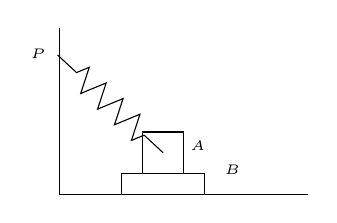
\begin{tikzpicture}[x=0.75pt,y=0.75pt,yscale=-1,xscale=1]
%uncomment if require: \path (0,300); %set diagram left start at 0, and has height of 300

%Straight Lines [id:da7861775888075377] 
\draw    (120,70) -- (120,150) ;
%Straight Lines [id:da5304720563417415] 
\draw    (240,150) -- (120,150) ;
%Shape: Rectangle [id:dp0651080644636306] 
\draw   (150,140) -- (190,140) -- (190,150) -- (150,150) -- cycle ;
%Shape: Rectangle [id:dp9356085279332966] 
\draw   (160,120) -- (180,120) -- (180,140) -- (160,140) -- cycle ;
%Shape: Resistor [id:dp8622106164753849] 
\draw   (119.11,82.88) -- (128.27,91.36) -- (134.41,88.82) -- (130.28,101.44) -- (142.55,96.36) -- (138.42,108.98) -- (150.69,103.9) -- (146.56,116.52) -- (158.83,111.44) -- (154.71,124.06) -- (160.84,121.52) -- (170,130) ;

% Text Node
\draw (105,79) node [anchor=north west][inner sep=0.75pt]  [font=\tiny] [align=left] {$\displaystyle P$};
% Text Node
\draw (182,123) node [anchor=north west][inner sep=0.75pt]  [font=\tiny] [align=left] {$\displaystyle A$};
% Text Node
\draw (198.5,134.5) node [anchor=north west][inner sep=0.75pt]  [font=\tiny] [align=left] {$\displaystyle B$};


\end{tikzpicture}

\end{center}
~\\

\end{minipage}
~\\

记$F_{BA}$为B对A摩擦力,$F_{AB}$为A对B摩擦力,$f$为地面对B摩擦力。对B受力分析,水平方向有$F_{BA}=F_{AB}=f$,$f$与$F_{AB}$方向相反。由牛顿第三定律$F_{BA}$与$F_{AB}$大小相同方向相反,故$F_{BA}$与$f$同向,AB正确。

\begin{center}
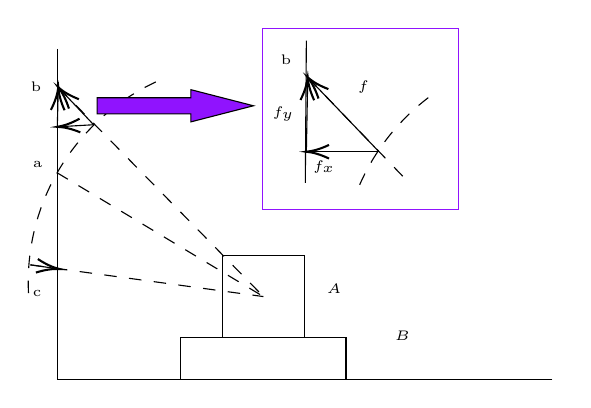
\begin{tikzpicture}[x=0.75pt,y=0.75pt,yscale=-1,xscale=1]
%uncomment if require: \path (0,300); %set diagram left start at 0, and has height of 300

%Straight Lines [id:da7861775888075377] 
\draw    (127.92,70) -- (127.92,229.06) ;
%Straight Lines [id:da5304720563417415] 
\draw    (366.5,229.06) -- (127.92,229.06) ;
%Shape: Rectangle [id:dp0651080644636306] 
\draw   (187.56,209.17) -- (267.09,209.17) -- (267.09,229.06) -- (187.56,229.06) -- cycle ;
%Shape: Rectangle [id:dp9356085279332966] 
\draw   (207.44,169.41) -- (247.21,169.41) -- (247.21,209.17) -- (207.44,209.17) -- cycle ;
%Straight Lines [id:da08747233001019916] 
\draw  [dash pattern={on 4.5pt off 4.5pt}]  (127.92,129.65) -- (227.33,189.29) ;
%Shape: Arc [id:dp811197777514447] 
\draw  [draw opacity=0][dash pattern={on 4.5pt off 4.5pt}] (114.13,187.58) .. controls (114.04,185.84) and (114,184.09) .. (114,182.33) .. controls (114,138.75) and (140.21,101.29) .. (177.72,84.86) -- (220.37,182.33) -- cycle ; \draw  [dash pattern={on 4.5pt off 4.5pt}] (114.13,187.58) .. controls (114.04,185.84) and (114,184.09) .. (114,182.33) .. controls (114,138.75) and (140.21,101.29) .. (177.72,84.86) ;  
%Straight Lines [id:da821105564499153] 
\draw  [dash pattern={on 4.5pt off 4.5pt}]  (128.5,88.5) -- (227.33,189.29) ;
%Straight Lines [id:da3172876609897355] 
\draw  [dash pattern={on 4.5pt off 4.5pt}]  (115,174) -- (227.33,189.29) ;
%Straight Lines [id:da13078526853284989] 
\draw    (115,174) -- (127.02,175.72) ;
\draw [shift={(129,176)}, rotate = 188.13] [color={rgb, 255:red, 0; green, 0; blue, 0 }  ][line width=0.75]    (10.93,-3.29) .. controls (6.95,-1.4) and (3.31,-0.3) .. (0,0) .. controls (3.31,0.3) and (6.95,1.4) .. (10.93,3.29)   ;
%Straight Lines [id:da7594860798135725] 
\draw    (145.5,106.5) -- (129.87,89.95) ;
\draw [shift={(128.5,88.5)}, rotate = 46.64] [color={rgb, 255:red, 0; green, 0; blue, 0 }  ][line width=0.75]    (10.93,-3.29) .. controls (6.95,-1.4) and (3.31,-0.3) .. (0,0) .. controls (3.31,0.3) and (6.95,1.4) .. (10.93,3.29)   ;
%Straight Lines [id:da09715861513592183] 
\draw    (145.5,106.5) -- (130,107.39) ;
\draw [shift={(128,107.5)}, rotate = 356.73] [color={rgb, 255:red, 0; green, 0; blue, 0 }  ][line width=0.75]    (10.93,-3.29) .. controls (6.95,-1.4) and (3.31,-0.3) .. (0,0) .. controls (3.31,0.3) and (6.95,1.4) .. (10.93,3.29)   ;
%Straight Lines [id:da44184320458819637] 
\draw    (128,107.5) -- (128.45,90.5) ;
\draw [shift={(128.5,88.5)}, rotate = 91.51] [color={rgb, 255:red, 0; green, 0; blue, 0 }  ][line width=0.75]    (10.93,-3.29) .. controls (6.95,-1.4) and (3.31,-0.3) .. (0,0) .. controls (3.31,0.3) and (6.95,1.4) .. (10.93,3.29)   ;
%Right Arrow [id:dp8828358304273138] 
\draw  [color={rgb, 255:red, 0; green, 0; blue, 0 }  ,draw opacity=1 ][fill={rgb, 255:red, 144; green, 19; blue, 254 }  ,fill opacity=1 ] (147.22,93.48) -- (192.39,93.48) -- (192.39,89.61) -- (222.5,97.36) -- (192.39,105.11) -- (192.39,101.23) -- (147.22,101.23) -- cycle ;
%Straight Lines [id:da20912405831906367] 
\draw    (248,66) -- (247.5,134.5) ;
%Straight Lines [id:da08777511782663772] 
\draw  [dash pattern={on 4.5pt off 4.5pt}]  (248.67,83.71) -- (297.5,134.5) ;
%Shape: Arc [id:dp6530050202868027] 
\draw  [draw opacity=0][dash pattern={on 4.5pt off 4.5pt}] (273.68,135.43) .. controls (281.76,117.03) and (294.9,101.34) .. (311.34,90.15) -- (371.13,178.13) -- cycle ; \draw  [dash pattern={on 4.5pt off 4.5pt}] (273.68,135.43) .. controls (281.76,117.03) and (294.9,101.34) .. (311.34,90.15) ;  
%Straight Lines [id:da04960792127568481] 
\draw    (283,119.5) -- (250.06,85.15) ;
\draw [shift={(248.67,83.71)}, rotate = 46.2] [color={rgb, 255:red, 0; green, 0; blue, 0 }  ][line width=0.75]    (10.93,-3.29) .. controls (6.95,-1.4) and (3.31,-0.3) .. (0,0) .. controls (3.31,0.3) and (6.95,1.4) .. (10.93,3.29)   ;
%Straight Lines [id:da6269010961403325] 
\draw    (283,119.5) -- (250,119.5) ;
\draw [shift={(248,119.5)}, rotate = 360] [color={rgb, 255:red, 0; green, 0; blue, 0 }  ][line width=0.75]    (10.93,-3.29) .. controls (6.95,-1.4) and (3.31,-0.3) .. (0,0) .. controls (3.31,0.3) and (6.95,1.4) .. (10.93,3.29)   ;
%Straight Lines [id:da0397091070463389] 
\draw    (248,119.5) -- (248.64,85.71) ;
\draw [shift={(248.67,83.71)}, rotate = 91.08] [color={rgb, 255:red, 0; green, 0; blue, 0 }  ][line width=0.75]    (10.93,-3.29) .. controls (6.95,-1.4) and (3.31,-0.3) .. (0,0) .. controls (3.31,0.3) and (6.95,1.4) .. (10.93,3.29)   ;
%Shape: Rectangle [id:dp5523513755058833] 
\draw  [color={rgb, 255:red, 144; green, 19; blue, 254 }  ,draw opacity=1 ] (227,60) -- (321.5,60) -- (321.5,147.5) -- (227,147.5) -- cycle ;

% Text Node
\draw (256.62,181.8) node [anchor=north west][inner sep=0.75pt]  [font=\tiny] [align=left] {$\displaystyle A$};
% Text Node
\draw (289.43,204.66) node [anchor=north west][inner sep=0.75pt]  [font=\tiny] [align=left] {$\displaystyle B$};
% Text Node
\draw (115,123) node [anchor=north west][inner sep=0.75pt]  [font=\tiny] [align=left] {a};
% Text Node
\draw (114,84.5) node [anchor=north west][inner sep=0.75pt]  [font=\tiny] [align=left] {b};
% Text Node
\draw (115,185) node [anchor=north west][inner sep=0.75pt]  [font=\tiny] [align=left] {c};
% Text Node
\draw (271.5,84) node [anchor=north west][inner sep=0.75pt]  [font=\tiny] [align=left] {$\displaystyle f$};
% Text Node
\draw (230.5,96.5) node [anchor=north west][inner sep=0.75pt]  [font=\tiny] [align=left] {$\displaystyle f_{y}$};
% Text Node
\draw (250,122.5) node [anchor=north west][inner sep=0.75pt]  [font=\tiny] [align=left] {$\displaystyle f_{x}$};
% Text Node
\draw (234.5,71.5) node [anchor=north west][inner sep=0.75pt]  [font=\tiny] [align=left] {b};


\end{tikzpicture}

\end{center}

如图所示,由于题目中并未告诉我们弹簧原长位置,故我们随便假设一点a为弹簧原长位置,由于物块A、B保持静止,弹簧另一端在竖直面上移动,故以A中心为圆心,到a距离为半径,作圆。现取高于a点的b点分析,根据前文所述,我们可以画出弹力的示意图,并对其进行分解,如图中小图所示。从b下移到a的过程中,由图可以看出,弹力$f$先减小在增大(过a点后增大),其分量$f_x$、$f_y$也先减小后增大(注意过a点后两个分量方向与在b点方向相反)。


故我们可知,从b到c的过程中,地面对B摩擦力$f$先减小后增大,地面对B压力$N$一直增大($f_y$过a点后反向)。


但原题中并未告知我们初始P点在原长位置(a点)上方还是下方,故有多种可能,CD均错。


综上所述,选AB。
\end{ep}

\section{类抛体最远射程若干解法}

在涉及到抛体运动或类抛体运动的最远射程问题时,在高中一般情况下会联立运动学方程求解得出射程$L$与抛射角$\theta$的函数关系,对其关于$\theta$求导并带入求得射程最值亦或者使用三角函数运算运用三角函数的值域求解出射程最值。这两种方法或多或少都涉及到了较复杂的数学运算,在此介绍两种方法,可以在不进行复杂的求导或三角函数运算下求解此类问题。


\begin{ep}{自编题}{}

\begin{center}
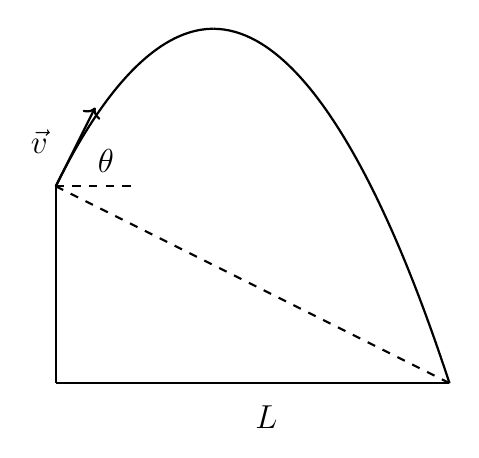
\begin{tikzpicture} 
\draw [thick] (2,2) parabola (5,-2.5);
\draw [thick] (0,0) parabola[bend at end] (2,2);
\draw [thick] (0,0) -- (0, -2.5); 
\draw [dashed,thick] (0,0) -- (5, -2.5); 
\draw [thick] (0,-2.5) -- (5, -2.5); 
\draw [thick] (0,-2.5) -- (5, -2.5); 
\draw [thick,->] (0,0) -- (0.5, 1); 
\draw [dashed,thick] (0,0) -- (1, 0);
\draw (0.5,0.5) node [anchor=north west][inner sep=0.75pt][font=\large][align=left] {$\theta$};
\draw (-0.35,0.75) node [anchor=north west][inner sep=0.75pt][font=\large][align=left] {$\vec{v}$};
\draw (2.5,-2.75) node [anchor=north west][inner sep=0.75pt][font=\large][align=left] {$L$};
\end{tikzpicture} 
\end{center}

如图所示,现在假设在一个高为$h$的平台上抛球,抛出的速度恒定为$v$,抛射仰角为$\theta$,抛出距离为$L$,重力加速度竖直向下为$g$,现试求出抛出距离最大值$L_{max}$以及此时抛射角$\theta_0$.
~\\

由于无论落在何处,落点与抛点的高度差恒为$h$,故落点速度恒为$v^{\prime} = \sqrt{v^2 + 2gh}$。我们可以绘出如下速度三角形

\begin{center}

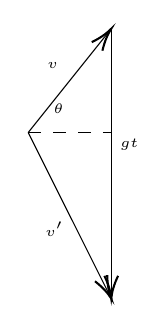
\begin{tikzpicture}[x=0.75pt,y=0.75pt,yscale=-1,xscale=1]
%uncomment if require: \path (0,300); %set diagram left start at 0, and has height of 300

%Straight Lines [id:da46243992269866174] 
\draw    (300,140) -- (338.75,91.56) ;
\draw [shift={(340,90)}, rotate = 128.66] [color={rgb, 255:red, 0; green, 0; blue, 0 }  ][line width=0.75]    (10.93,-3.29) .. controls (6.95,-1.4) and (3.31,-0.3) .. (0,0) .. controls (3.31,0.3) and (6.95,1.4) .. (10.93,3.29)   ;
%Straight Lines [id:da8785074955834897] 
\draw    (300,140) -- (339.11,218.21) ;
\draw [shift={(340,220)}, rotate = 243.43] [color={rgb, 255:red, 0; green, 0; blue, 0 }  ][line width=0.75]    (10.93,-3.29) .. controls (6.95,-1.4) and (3.31,-0.3) .. (0,0) .. controls (3.31,0.3) and (6.95,1.4) .. (10.93,3.29)   ;
%Straight Lines [id:da6190778526626308] 
\draw    (340,90) -- (340,218) ;
\draw [shift={(340,220)}, rotate = 270] [color={rgb, 255:red, 0; green, 0; blue, 0 }  ][line width=0.75]    (10.93,-3.29) .. controls (6.95,-1.4) and (3.31,-0.3) .. (0,0) .. controls (3.31,0.3) and (6.95,1.4) .. (10.93,3.29)   ;
%Straight Lines [id:da631938576081565] 
\draw  [dash pattern={on 4.5pt off 4.5pt}]  (300,140) -- (340,140) ;

% Text Node
\draw (308,105) node [anchor=north west][inner sep=0.75pt]  [font=\tiny] [align=left] {$\displaystyle v$};
% Text Node
\draw (307,182) node [anchor=north west][inner sep=0.75pt]  [font=\tiny] [align=left] {$\displaystyle v^{\prime }$};
% Text Node
\draw (343,142) node [anchor=north west][inner sep=0.75pt]  [font=\tiny] [align=left] {$\displaystyle gt$};
% Text Node
\draw (311,125) node [anchor=north west][inner sep=0.75pt]  [font=\tiny] [align=left] {$\displaystyle \theta $};


\end{tikzpicture}


\end{center}

这个三角形的面积$S=\frac{1}{2} v \cos \theta gt = \frac{1}{2} g L$,可见,当三角形面积$S$最大时,$L$最大。三角形两边$v$、$v^{\prime}$长度固定,当这两边相互垂直时,$S$取得最大。故

$$S_{max} = \frac{1}{2} v v^{\prime} = \frac{1}{2} g L_{max}$$

解得$L_{max} = \frac{v v^{\prime}}{g} = \frac{v\sqrt{v^2 + 2gh}}{g}$,并且此时根据相似三角形可得$\theta_0 = \arctan{\frac{v}{v^{\prime}}} = \arctan{\frac{v}{\sqrt{v^2 + 2gh}}}$

\end{ep}

对于第二种解法,需要一个定理,如下

\begin{center}
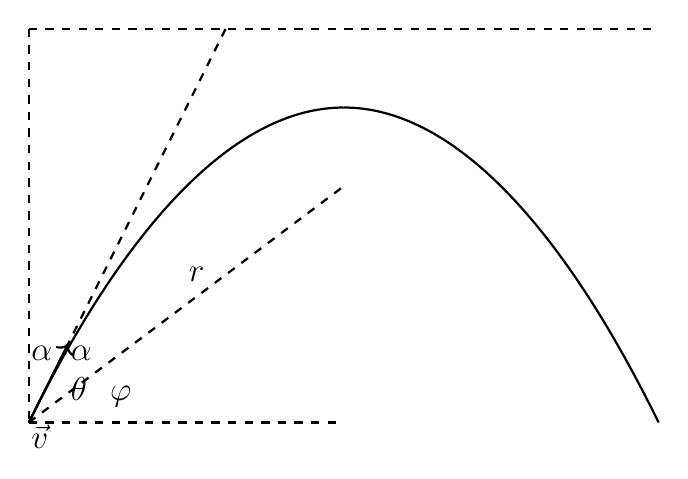
\begin{tikzpicture} 
\draw [thick] (-4,-5) parabola[bend at end] (0,-1);
\draw [thick] (4,-5) parabola[bend at end] (0,-1);
\draw [dashed,thick] (-4,-5) -- (0,-2); 
\draw [dashed,thick] (-4,0) -- (4,0); 
\draw [dashed,thick] (-4,0) -- (-4,-5); 
\draw [dashed,thick] (-4,-5) -- (0,-5);
\draw [dashed,thick] (-4,-5) -- (-1.5,0);
\draw [thick,->] (-4,-5) -- (-3.5, -4); 
\draw (-2,-3) node [anchor=north west][inner sep=0.75pt][font=\large][align=left] {$r$};
\draw (-4,-4) node [anchor=north west][inner sep=0.75pt][font=\large][align=left] {$\alpha$};
\draw (-3.5,-4) node [anchor=north west][inner sep=0.75pt][font=\large][align=left] {$\alpha$};
\draw (-3,-4.5) node [anchor=north west][inner sep=0.75pt][font=\large][align=left] {$\varphi$};
\draw (-3.5,-4.4) node [anchor=north west][inner sep=0.75pt][font=\large][align=left] {$\theta$};
\draw (-4,-5) node [anchor=north west][inner sep=0.75pt][font=\large][align=left] {$\vec{v}$};
\end{tikzpicture}
\end{center}

对于任意抛体运动,记某时刻物体速度大小为$v$,物体到焦点距离为$r$,物体与焦点连线与水平面夹角$\varphi$,速度与水平面夹角$\theta$,由抛物线几何性质易知,抛物线切线(也就是速度的延长线)平分物体与焦点连线与物体对准线所作垂线所形成的角,记平分后的两个角为$\alpha$,从该位置到抛物线顶点的过程我们可以列如下方程。

\begin{subequations}
\begin{align*}
\theta + \alpha &= \varphi + 2 \alpha = \frac{\pi}{2} \\
r \cos \varphi &= v \cos \theta t \\
v \sin \theta &= gt 
\end{align*}
\end{subequations}

联立上式,解得$v^2 = 2gr$。故

\begin{theo}[label=d_ptydjbj]{抛体运动速度与焦半径关系}{}
对于任一抛体运动,任意时刻速度$v$与该物体到焦点距离$r$满足

$$v^2 = 2gr$$

\end{theo}

对于竖直上抛,可以认为为焦准距为$0$的抛物线,此时$r$等于到顶点距离,上式便可从能量守恒推出。

运用此定理,我们可以很快解出之前的问题。

\begin{ep}{接上题,方法二}{}
由于无论落在何处,落点与抛点的高度差恒为$h$,故落点速度恒为$v^{\prime} = \sqrt{v^2 + 2gh}$。
根据前文定理,可知抛点到焦点距离为定值,落点到焦点距离也为定值。根据三角形两边之和大于第三边知,当抛点,焦点,落点三点共线时,落点到抛点距离最远,此时$L_{max}$,故

$$L_{max} = \sqrt{\frac{1}{4g^2} (v^2 + {v^{\prime}}^2)^2 - h^2} = \frac{v\sqrt{v^2 + 2gh}}{g}$$

此时列出运动学方程,可解出$\theta_0 = \arctan{\frac{v}{\sqrt{v^2 + 2gh}}}$
\end{ep}

我们不难发现,\textbf{如果题目要求从某定点过另一定点,且已知这两点高度差(或者经过这两点的速度的关系),求速度的最小值,那么均可以使用\theoref{d_ptydjbj}快速解决},运用此定理还可以解决方法一解决不了的问题,如下

\begin{ep}{练习题(有删减)}{}

\begin{center}
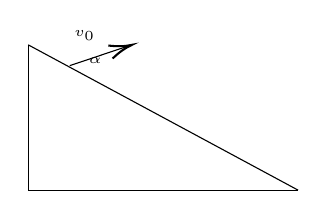
\begin{tikzpicture}[x=0.75pt,y=0.75pt,yscale=-1,xscale=1]
%uncomment if require: \path (0,300); %set diagram left start at 0, and has height of 300

%Straight Lines [id:da9469337076591173] 
\draw    (280,110) -- (280,180) ;
%Straight Lines [id:da17421041915784108] 
\draw    (280,180) -- (410,180) ;
%Straight Lines [id:da6864576612415993] 
\draw    (410,180) -- (280,110) ;
%Straight Lines [id:da311962285159086] 
\draw    (300,120) -- (328.1,110.63) ;
\draw [shift={(330,110)}, rotate = 161.57] [color={rgb, 255:red, 0; green, 0; blue, 0 }  ][line width=0.75]    (10.93,-3.29) .. controls (6.95,-1.4) and (3.31,-0.3) .. (0,0) .. controls (3.31,0.3) and (6.95,1.4) .. (10.93,3.29)   ;

% Text Node
\draw (308,115) node [anchor=north west][inner sep=0.75pt]  [font=\tiny] [align=left] {$\displaystyle \alpha $};
% Text Node
\draw (301,102) node [anchor=north west][inner sep=0.75pt]  [font=\tiny] [align=left] {$\displaystyle v_{0}$};


\end{tikzpicture}

\end{center}

某同学设计了一款小游戏,在倾角为$\theta = 30^{\circ}$的斜面顶端A安装一个玩具小枪,可以在竖直面内沿各个方向射出速度大小均为$v_0 = \frac{\sqrt{3gL}}{2}$的子弹,当子弹射出方向与斜面垂直时,子弹落在斜面上离A点距离为$L$的P点(图中未画出),不计空气阻力,重力加速度为$g$,斜面足够长,要使于弹落在斜面上时离A点最远,子弹射出时的速度与斜面间的夹角应多大,最远距离为多少?
~\\

设最远距离为$L_{max}$,则落点速度$v$满足

$$\frac{1}{2} m v_0^2 + mgL_{max} \sin 30^{\circ} = \frac{1}{2} m v^2$$

根据前文定理,易知当抛点,焦点,落点三点共线时,落点到抛点距离最远,故

$$2gL_{max} = v_0^2 + v^2$$

联立,带入$v_0$,解得$L_{max} = \frac{4 v_0^2}{3g}$。由运动学定理

$$2 v_0 \sin \alpha = g \cos \theta t ,\quad L_{max} = \frac{1}{2} g \sin \theta t^2 + v_0 t \cos \theta$$

解得$\alpha = 30^{\circ}$

\end{ep}

\section{换系}

\subsection{速度及加速度牵连}
\label{s_sdql}

在高中,我们解题一般取地面参考系进行分析,但有时选取另一个参考系可以简化我们的分析过程。

\begin{center}

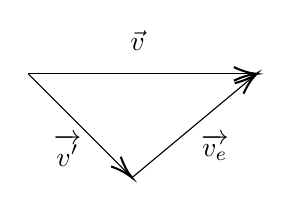
\begin{tikzpicture}[x=0.75pt,y=0.75pt,yscale=-1,xscale=1]
%uncomment if require: \path (0,300); %set diagram left start at 0, and has height of 300

%Straight Lines [id:da7991902571121818] 
\draw    (130,100) -- (238,100) ;
\draw [shift={(240,100)}, rotate = 180] [color={rgb, 255:red, 0; green, 0; blue, 0 }  ][line width=0.75]    (10.93,-3.29) .. controls (6.95,-1.4) and (3.31,-0.3) .. (0,0) .. controls (3.31,0.3) and (6.95,1.4) .. (10.93,3.29)   ;
%Straight Lines [id:da14174806175529686] 
\draw    (130,100) -- (178.59,148.59) ;
\draw [shift={(180,150)}, rotate = 225] [color={rgb, 255:red, 0; green, 0; blue, 0 }  ][line width=0.75]    (10.93,-3.29) .. controls (6.95,-1.4) and (3.31,-0.3) .. (0,0) .. controls (3.31,0.3) and (6.95,1.4) .. (10.93,3.29)   ;
%Straight Lines [id:da019391773911319188] 
\draw    (180,150) -- (238.46,101.28) ;
\draw [shift={(240,100)}, rotate = 140.19] [color={rgb, 255:red, 0; green, 0; blue, 0 }  ][line width=0.75]    (10.93,-3.29) .. controls (6.95,-1.4) and (3.31,-0.3) .. (0,0) .. controls (3.31,0.3) and (6.95,1.4) .. (10.93,3.29)   ;

% Text Node
\draw (178,78) node [anchor=north west][inner sep=0.75pt]   [align=left] {$\displaystyle \vec{v}$};
% Text Node
\draw (141,128) node [anchor=north west][inner sep=0.75pt]   [align=left] {$\displaystyle \overrightarrow{v^{\prime }}$};
% Text Node
\draw (212,128) node [anchor=north west][inner sep=0.75pt]   [align=left] {$\displaystyle \overrightarrow{v_{e}}$};


\end{tikzpicture}

\end{center}

\begin{theo}{换系速度牵连}{}
现在我们假设有一物体在空间中运动,在地面系中观察,其速度为$\vec{v}$,在一个相对地面以$\vec{v_e}$速度运动的惯性系中观察,其速度为$\vec{v^{\prime}}$。则有如下速度牵连:

$$\vec{v} = \vec{v^{\prime}} + \vec{v_e}$$

我们称地面系中速度$\vec{v}$为\textbf{绝对速度},新参考系中速度$\vec{v^{\prime}}$为\textbf{相对速度},参考系之间相对速度$\vec{v_e}$为\textbf{牵连速度}。则有
\begin{center}
\textbf{相对速度加牵连速度等于绝对速度}
\end{center}

\end{theo}

类比上式,我们可以得到在直线匀加速参考系中加速度牵连关系

\begin{theo}{换系加速度牵连}{}
现在我们假设有一物体在空间中运动,在地面系中观察,其加速度为$\vec{a}$,在一个相对地面以$\vec{a_e}$的加速度平动且没有转动的参考系中观察,其加速度为$\vec{a^{\prime}}$。则有如下加速度牵连:
$$\vec{a} = \vec{a^{\prime}} + \vec{a_e}$$
\end{theo}

\begin{ep}{练习题}{}
如图所示,河的宽度为$L$。河水流速为$u$,"。A、B两船均以静水中的速度$v$同时渡河。出发时两船相距$2L$。A、B两船船头均与岸边成$60^{\circ}$角,B恰好到达正对于出发点的a点。则下列判断正确的是()

\begin{minipage}[b]{0.65\linewidth}
\begin{enumerate}[label=(\Alph*)]
  \item A船正好也在a点靠岸
  \item A船在a点下游靠岸
  \item A、B两船到达对岸的时间相等
  \item A、B两船可能在未到达对岸前相遇
\end{enumerate}
\end{minipage}
\hfill
\begin{minipage}[b]{0.3\linewidth}
\begin{center}
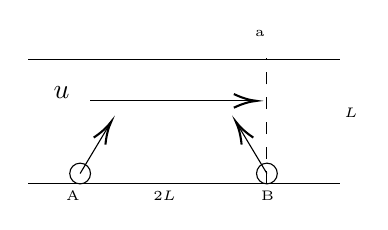
\begin{tikzpicture}[x=0.75pt,y=0.75pt,yscale=-1,xscale=1]
%uncomment if require: \path (0,300); %set diagram left start at 0, and has height of 300

%Straight Lines [id:da21927273521379798] 
\draw    (120,80) -- (270,80) ;
%Straight Lines [id:da4378923778307051] 
\draw    (120,140) -- (270,140) ;
%Shape: Circle [id:dp7352837546468081] 
\draw   (140,135) .. controls (140,132.24) and (142.24,130) .. (145,130) .. controls (147.76,130) and (150,132.24) .. (150,135) .. controls (150,137.76) and (147.76,140) .. (145,140) .. controls (142.24,140) and (140,137.76) .. (140,135) -- cycle ;
%Shape: Circle [id:dp41722119373569155] 
\draw   (230,135) .. controls (230,132.24) and (232.24,130) .. (235,130) .. controls (237.76,130) and (240,132.24) .. (240,135) .. controls (240,137.76) and (237.76,140) .. (235,140) .. controls (232.24,140) and (230,137.76) .. (230,135) -- cycle ;
%Straight Lines [id:da7158120985157417] 
\draw    (145,135) -- (158.97,111.71) ;
\draw [shift={(160,110)}, rotate = 120.96] [color={rgb, 255:red, 0; green, 0; blue, 0 }  ][line width=0.75]    (10.93,-3.29) .. controls (6.95,-1.4) and (3.31,-0.3) .. (0,0) .. controls (3.31,0.3) and (6.95,1.4) .. (10.93,3.29)   ;
%Straight Lines [id:da9687396877898515] 
\draw    (235,135) -- (221.03,111.71) ;
\draw [shift={(220,110)}, rotate = 59.04] [color={rgb, 255:red, 0; green, 0; blue, 0 }  ][line width=0.75]    (10.93,-3.29) .. controls (6.95,-1.4) and (3.31,-0.3) .. (0,0) .. controls (3.31,0.3) and (6.95,1.4) .. (10.93,3.29)   ;
%Straight Lines [id:da22872254896655053] 
\draw    (150,100) -- (228,100) ;
\draw [shift={(230,100)}, rotate = 180] [color={rgb, 255:red, 0; green, 0; blue, 0 }  ][line width=0.75]    (10.93,-3.29) .. controls (6.95,-1.4) and (3.31,-0.3) .. (0,0) .. controls (3.31,0.3) and (6.95,1.4) .. (10.93,3.29)   ;
%Straight Lines [id:da5167178486268149] 
\draw  [dash pattern={on 4.5pt off 4.5pt}]  (235,140) -- (235,79.5) ;

% Text Node
\draw (271,102) node [anchor=north west][inner sep=0.75pt]  [font=\tiny] [align=left] {$\displaystyle L$};
% Text Node
\draw (137,142) node [anchor=north west][inner sep=0.75pt]  [font=\tiny] [align=left] {A};
% Text Node
\draw (231,142) node [anchor=north west][inner sep=0.75pt]  [font=\tiny] [align=left] {B};
% Text Node
\draw (179,142) node [anchor=north west][inner sep=0.75pt]  [font=\tiny] [align=left] {$\displaystyle 2L$};
% Text Node
\draw (131,92) node [anchor=north west][inner sep=0.75pt]   [align=left] {$\displaystyle u$};
% Text Node
\draw (228,65) node [anchor=north west][inner sep=0.75pt]  [font=\tiny] [align=left] {a};


\end{tikzpicture}

\end{center}
~\\
\end{minipage}
~\\

A、B两船垂直于河岸的分速度均为$v \sin 60^{\circ}$,故两船到达对岸时间相同,均为$t=\frac{L}{v \sin 60^{\circ}}$,C对。由于B船到达正对于出发点的a点,故$u = v \cos 60^{\circ} = \frac{v}{2}$。以B为参考,则A船的速度为$u + v \cos 60^{\circ} = v$,走过的水平距离为$v t = \frac{L}{\sin 60^{\circ}} = \frac{2 \sqrt{3} L}{3} < 2L$,故A船无法与B船相遇,无法过a点,因此ABD错。综上所述,答案为C。
\end{ep}

\subsection{惯性力}
\label{s_gxl}

若物体相对地面存在一个加速度$\vec{a}$,则物体所受合外力$\vec{F}$满足牛顿第二定理$\vec{F}=m \vec{a}$,其中$m$为物体质量。

\begin{defi}{惯性力}{}
有一个质量为$m$的物体在地面系中以$\vec{a}$加速运动,在相对地面以加速度$\vec{a}$做变速运动的参考系中,定义$\vec{f_e}=-m \vec{a}$为在加速参考系中该物体惯性力。则有$\vec{F}+\vec{f_e} = \vec{0}$(相当于在地面系中列式后移项)。

注意惯性力$\vec{f_e}$的方向与$\vec{a}$的方向相反。
\end{defi}

惯性力的作用在于将一个动力学问题转化为一个静力学问题,从而可以使用矢量三角形等图解方法进行分析,从从而简化解题过程。

\subsection{约化质量}
\label{s_yhzl}

设在惯性系中有两个物体A、B,其质量分别为$m_A$、$m_B$,位矢分别为$\vec{r_A}$、$\vec{r_B}$。该二体系统不受外力,但之间有内力。设A对B的力为$\vec{F_{AB}}$,B对A的力为$\vec{F_{BA}}$,由牛顿第三定律知$\vec{F} = \vec{F_{AB}} = - \vec{F_{BA}}$。故有
\begin{subequations}
\begin{align*}
\vec{a_A} &= \frac{d^2 \vec{r_A}}{d t^2} = m_A \vec{F_{BA}}  \\
\vec{a_B} &= \frac{d^2 \vec{r_B}}{d t^2} = m_B \vec{F_{AB}}  
\end{align*}
\end{subequations}

现取物体A为参考系,观察物体B的运动,则有
\begin{subequations}
\begin{align*}
\frac{d^2 (\vec{r_B} - \vec{r_A})}{d t^2} &= \frac{\vec{F_{AB}}}{m_B} - \frac{\vec{F_{BA}}}{m_A} \\
&= (\frac{1}{m_B} + \frac{1}{m_A}) \vec{F} \\
&= \frac{\vec{F}}{\mu}
\end{align*}
\end{subequations}
其中$\mu = \frac{m_A m_B}{m_A + m_B}$为约化质量\footnote{有时“约化质量”也被称为“调和质量”、“折合质量”、“并联质量”。笔者青睐于称其为“调和质量”,因其反映了该质量的更本质的物理意义与对称性,但为了与其他资料相同,还是称其为更广泛使用的“约化质量”。}。

\begin{defi}{约化质量}{}
在一个两体问题中,设这两个物体质量分别为$m_A$、$m_B$,则定义约化质量$\mu$为

$$\mu = \frac{m_A m_B}{m_A + m_B}$$

记忆方法为:\textbf{“积”在“和”上飞(鸡在河上飞)}
\end{defi}

对于一个二体问题,我们可以用约化质量将一个两体问题转化为一个一体问题,从而简化分析和计算。在高中最常见的二体问题便是双星运动

\begin{ep}{自编题}{}
在宇宙中存在一双星系统,两星质量分别为$m_1$、$m_2$,间距为$L$,绕着公共圆心以角速度$\omega$旋转,试写出$m_1$、$m_2$、$L$、$\omega$之间关系
~\\

两星之间吸引力为$F = \frac{G m_1 m_2}{L^2}$

现取其中一星为参考系,观察另一星的运动,则有

$$F = \mu \omega^2 L$$

其中$\mu = \frac{m_1 m_2}{m_1 + m_2}$,联立上面两式,解得

\begin{equation}
\boxed{G (m_1 + m_2) = \omega^2 L^3}
\end{equation}

\end{ep}

\begin{mk}{易错提醒}{}
约化质量只可在运动学分析中使用,\textbf{不可在万有引力计算中使用}。约化质量只是等效的质量,并非实际的质量。
\end{mk}
\section{质心系}

\subsection{质心}

若一个系统由多个质点组成,其整个系统的质量可等效集中于一点,即质心。

\begin{defi}[label=zxdy]{质心}{}
若各质点质量与坐标分别为$m_1$、$(x_1,y_1)$,$m_2$、$(x_2,y_2)$……$m_n$、$(x_n,y_n)$,则质心位置为
$$x_c = \frac{\sum m_i x_i}{\sum m_i} ,\quad y_c = \frac{\sum m_i y_i}{\sum m_i}$$
\end{defi}

质心在物理中有很多应用,如如果重力场是匀强场($g$为定值),则重心与质心重合,因此,重力势能的变化可以利用质心来计算。

\begin{ep}{练习题}{}
\begin{center}
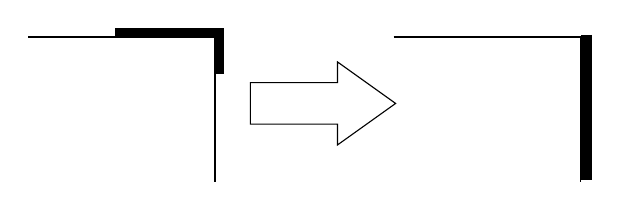
\begin{tikzpicture}[x=0.75pt,y=0.75pt,yscale=-1,xscale=1]
%uncomment if require: \path (0,300); %set diagram left start at 0, and has height of 300

%Straight Lines [id:da9215028484159156] 
\draw    (160,110) -- (250,110) -- (250,180) ;
%Straight Lines [id:da4977009583781107] 
\draw [line width=3.75]    (202,108) -- (252,108) -- (252,128) ;
%Straight Lines [id:da05737004026783943] 
\draw    (336,110) -- (426,110) -- (426,180) ;
%Right Arrow [id:dp10160418920196324] 
\draw   (267,132) -- (309,132) -- (309,122) -- (337,142) -- (309,162) -- (309,152) -- (267,152) -- cycle ;
%Straight Lines [id:da0051989052324770135] 
\draw [line width=3.75]    (429,109) -- (429,179) ;
\end{tikzpicture}
\end{center}
如图所示,有一总质量为$M=1kg$,总长度为$L=1m$的重绳,开始时有$L_0 = 0.2m$悬挂于桌边,后由于微扰重绳向右滑落,当重绳左端到达桌沿时,求重绳速度。(忽略重绳与桌面摩擦,桌子足够高以致重绳左端到达桌沿时右端未触地)
~\\

如图所示,选取桌面为零势能面,向下为正方向,记线密度$\lambda = \frac{M}{L} = 1kg/m$。

\begin{minipage}[b]{0.65\linewidth}
初态质心位置为
$$y_c = \frac{ 0 \cdot \lambda (L - L_0) + \frac{L_0}{2} \cdot \lambda L_0}{M}  = 0.02m$$
末态质心位置为
$$y_c^{\prime} = \frac{\frac{L}{2} \cdot \lambda L}{M} = 0.5m$$
由能量守恒可得$\frac{1}{2} M v^2 = Mg(y_c^{\prime}-y_c)$,解得$v = \frac{4\sqrt{15}}{5} m/s$
\end{minipage}
\hfill
\begin{minipage}[b]{0.35\linewidth}
\begin{center}
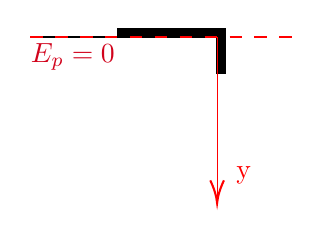
\begin{tikzpicture}[x=0.75pt,y=0.75pt,yscale=-1,xscale=1]
%uncomment if require: \path (0,300); %set diagram left start at 0, and has height of 300

%Straight Lines [id:da9215028484159156] 
\draw    (160,110) -- (250,110) -- (250,180) ;
%Straight Lines [id:da4977009583781107] 
\draw [line width=3.75]    (202,108) -- (252,108) -- (252,128) ;
%Straight Lines [id:da23325832635314958] 
\draw [color={rgb, 255:red, 255; green, 0; blue, 0 }  ,draw opacity=1 ]   (250,110) -- (250,188) ;
\draw [shift={(250,190)}, rotate = 270] [color={rgb, 255:red, 255; green, 0; blue, 0 }  ,draw opacity=1 ][line width=0.75]    (10.93,-3.29) .. controls (6.95,-1.4) and (3.31,-0.3) .. (0,0) .. controls (3.31,0.3) and (6.95,1.4) .. (10.93,3.29)   ;
%Straight Lines [id:da8953033878619383] 
\draw [color={rgb, 255:red, 255; green, 0; blue, 0 }  ,draw opacity=1 ] [dash pattern={on 4.5pt off 4.5pt}]  (160,110) -- (290,110) ;

% Text Node
\draw (258,171) node [anchor=north west][inner sep=0.75pt]  [color={rgb, 255:red, 255; green, 0; blue, 0 }  ,opacity=1 ] [align=left] {y};
% Text Node
\draw (159,112) node [anchor=north west][inner sep=0.75pt]   [align=left] {$\displaystyle \textcolor[rgb]{0.82,0.01,0.11}{E_{p} =0}$};
\end{tikzpicture}
\end{center}
\end{minipage}
\end{ep}

\subsection{质心与系统总动量}
质心还可用于求系统的总动量。由前文\defiref{zxdy},两端求导,得到($m_{tot}$为系统总质量\footnote{这里下标tot为total缩写})
\begin{subequations}
\begin{align*}
m_{tot} v_{cx} &= m_{tot} \frac{d x_c}{dt} = \sum m_i \frac{d x_c}{dt} = \sum m_i v_{ix} \\
m_{tot} v_{cy} &= m_{tot} \frac{d y_c}{dt} = \sum m_i \frac{d y_c}{dt} = \sum m_i v_{iy}  
\end{align*}
\end{subequations}

综上,有如下定理

\begin{theo}[label=zxyxtzdl]{质心与系统总动量}{}
一个系统的总动量等于系统总质量乘上质心速度,即$\vec{p} = m_{tot} \vec{v}$
\end{theo}

利用该定理,我们可以得到一个多星系统的很有用的结论
~\\

\begin{minipage}[b]{0.3\linewidth}
\begin{center}
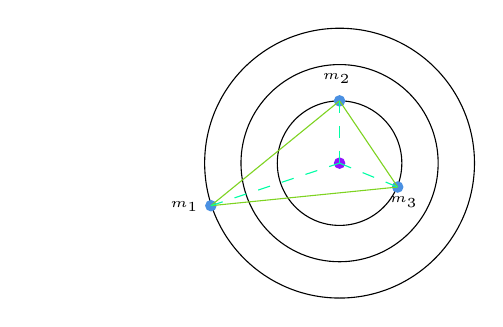
\begin{tikzpicture}[x=0.75pt,y=0.75pt,yscale=-1,xscale=1]
%uncomment if require: \path (0,300); %set diagram left start at 0, and has height of 300

%Straight Lines [id:da7411767697224816] 
\draw    (100,102) ;
%Shape: Circle [id:dp9490684003061072] 
\draw   (220,140) .. controls (220,123.43) and (233.43,110) .. (250,110) .. controls (266.57,110) and (280,123.43) .. (280,140) .. controls (280,156.57) and (266.57,170) .. (250,170) .. controls (233.43,170) and (220,156.57) .. (220,140) -- cycle ;
%Shape: Circle [id:dp9814343956363334] 
\draw   (202.5,140) .. controls (202.5,113.77) and (223.77,92.5) .. (250,92.5) .. controls (276.23,92.5) and (297.5,113.77) .. (297.5,140) .. controls (297.5,166.23) and (276.23,187.5) .. (250,187.5) .. controls (223.77,187.5) and (202.5,166.23) .. (202.5,140) -- cycle ;
%Shape: Circle [id:dp685701971148887] 
\draw   (185,140) .. controls (185,104.1) and (214.1,75) .. (250,75) .. controls (285.9,75) and (315,104.1) .. (315,140) .. controls (315,175.9) and (285.9,205) .. (250,205) .. controls (214.1,205) and (185,175.9) .. (185,140) -- cycle ;
%Shape: Circle [id:dp08570959225680785] 
\draw  [color={rgb, 255:red, 144; green, 19; blue, 254 }  ,draw opacity=1 ][fill={rgb, 255:red, 144; green, 19; blue, 254 }  ,fill opacity=1 ] (252.5,140) .. controls (252.5,138.62) and (251.38,137.5) .. (250,137.5) .. controls (248.62,137.5) and (247.5,138.62) .. (247.5,140) .. controls (247.5,141.38) and (248.62,142.5) .. (250,142.5) .. controls (251.38,142.5) and (252.5,141.38) .. (252.5,140) -- cycle ;
%Shape: Circle [id:dp47337912414359584] 
\draw  [color={rgb, 255:red, 74; green, 144; blue, 226 }  ,draw opacity=1 ][fill={rgb, 255:red, 74; green, 144; blue, 226 }  ,fill opacity=1 ] (280.5,151.5) .. controls (280.5,150.12) and (279.38,149) .. (278,149) .. controls (276.62,149) and (275.5,150.12) .. (275.5,151.5) .. controls (275.5,152.88) and (276.62,154) .. (278,154) .. controls (279.38,154) and (280.5,152.88) .. (280.5,151.5) -- cycle ;
%Shape: Circle [id:dp40050388744279153] 
\draw  [color={rgb, 255:red, 74; green, 144; blue, 226 }  ,draw opacity=1 ][fill={rgb, 255:red, 74; green, 144; blue, 226 }  ,fill opacity=1 ] (252.5,110) .. controls (252.5,108.62) and (251.38,107.5) .. (250,107.5) .. controls (248.62,107.5) and (247.5,108.62) .. (247.5,110) .. controls (247.5,111.38) and (248.62,112.5) .. (250,112.5) .. controls (251.38,112.5) and (252.5,111.38) .. (252.5,110) -- cycle ;
%Shape: Circle [id:dp5599587744609031] 
\draw  [color={rgb, 255:red, 74; green, 144; blue, 226 }  ,draw opacity=1 ][fill={rgb, 255:red, 74; green, 144; blue, 226 }  ,fill opacity=1 ] (190.5,160.5) .. controls (190.5,159.12) and (189.38,158) .. (188,158) .. controls (186.62,158) and (185.5,159.12) .. (185.5,160.5) .. controls (185.5,161.88) and (186.62,163) .. (188,163) .. controls (189.38,163) and (190.5,161.88) .. (190.5,160.5) -- cycle ;
%Straight Lines [id:da384151252822579] 
\draw [color={rgb, 255:red, 126; green, 211; blue, 33 }  ,draw opacity=1 ]   (188,160.5) -- (278,151.5) ;
%Straight Lines [id:da24848451118665693] 
\draw [color={rgb, 255:red, 126; green, 211; blue, 33 }  ,draw opacity=1 ]   (188,160.5) -- (250,110) ;
%Straight Lines [id:da8234484439529937] 
\draw [color={rgb, 255:red, 126; green, 211; blue, 33 }  ,draw opacity=1 ]   (250,110) -- (278,151.5) ;
%Straight Lines [id:da4853630824410369] 
\draw [color={rgb, 255:red, 0; green, 255; blue, 165 }  ,draw opacity=1 ] [dash pattern={on 4.5pt off 4.5pt}]  (188,160.5) -- (250,140) ;
%Straight Lines [id:da04897594598262511] 
\draw [color={rgb, 255:red, 0; green, 255; blue, 165 }  ,draw opacity=1 ] [dash pattern={on 4.5pt off 4.5pt}]  (250,140) -- (278,151.5) ;
%Straight Lines [id:da013808732174074745] 
\draw [color={rgb, 255:red, 0; green, 255; blue, 165 }  ,draw opacity=1 ] [dash pattern={on 4.5pt off 4.5pt}]  (250,110) -- (250,140) ;

% Text Node
\draw (167.33,157) node [anchor=north west][inner sep=0.75pt]  [font=\tiny] [align=left] {$\displaystyle m_{1}$};
% Text Node
\draw (240.67,95.33) node [anchor=north west][inner sep=0.75pt]  [font=\tiny] [align=left] {$ $$\displaystyle m_{2}$};
% Text Node
\draw (273,155) node [anchor=north west][inner sep=0.75pt]  [font=\tiny] [align=left] {$\displaystyle m_{3}$};


\end{tikzpicture}

\end{center}

\end{minipage}
\hfill
\begin{minipage}[b]{0.5\linewidth}
\begin{theo}{相对静止多星系统的公共圆心}{}
对于一个多星系统,若各星之间相对静止,则该多星系统的公共圆心为该系统质心
\end{theo}
\end{minipage}
~\\

对于如上定理,可用反证法证明,证明如下:

假定多星系统公共圆心不在质心处,则质心必定绕公共圆心做匀速圆周运动,那么根据之前的定理系统,系统总动量等于系统总质量乘上质心速度,故系统总质量方向将一直在变化。而该多星系统整体不受外力,因此系统总动量必须守恒,这与之前假设不符,故先前假设不成立,QED\footnote{QED为拉丁文quod erat demonstrandum的缩写,意为“证毕”}。

在大多数解析中,此类题目采取的思路是作最一般的位置假设,然后列方程计算。此定理跳过了繁琐的的方程求解,并令解题有了更强的方向性,不至于“无头苍蝇”。

\begin{mk}{易错提醒}{}
在此特别提醒,\textbf{万有引力计算绝不可以用质心},因为万有引力与距离关系不是一次函数关系,而是平方反比关系。\textbf{多星系统中某个天体向心力只能分别用万有引力定律计算相互之间引力,再利用平行四边形法则合成力}。
\end{mk}

\begin{ep}{练习题}{}
由三颗星体构成的系统,忽略其他星体对它们的作用,存在着种运动形式:三颗星体在相互之间的万有引力作用下,分别位于等边三角形的三个顶点上,绕某一共同的圆心$O$在三角形所在的平面内做相同角速度的圆周运动。若A星体的质量为$2m$,B、C两星体的质量均为$m$,三角形的边长为$a$,求:

\begin{enumerate}[label=(\arabic*)]
  \item A星体所受合力大小$F_A$;
  \item B星体所受合力大小$F_B$;
  \item C星体轨道半径$R_C$;
  \item 三星体做圆周运动周期$T$。
\end{enumerate}
~\\

\begin{minipage}[b]{0.65\linewidth}
(1) 如图所示,由万有引力公式$F_{BA}=F_{CA}=\frac{2 G m^2}{a^2}$,合力$F_A = \sqrt{3} F_{BA} = \frac{2\sqrt{3} G m^2}{a^2}$
~\\

(2) A对B引力$F_{AB}=\frac{2 G m^2}{a^2}$,C对B引力$F_{CB}=\frac{G m^2}{a^2}$,在矢量三角形中使用余弦定理,得
$$F_B = \sqrt{F_{AB}^2+F_{CB}^2-2F_{AB} \cdot F_{CB} \cos{120^{\circ}}}=\frac{\sqrt{7}G m^2}{a^2}$$
\end{minipage}
\hfill
\begin{minipage}[b]{0.35\linewidth}
\begin{center}
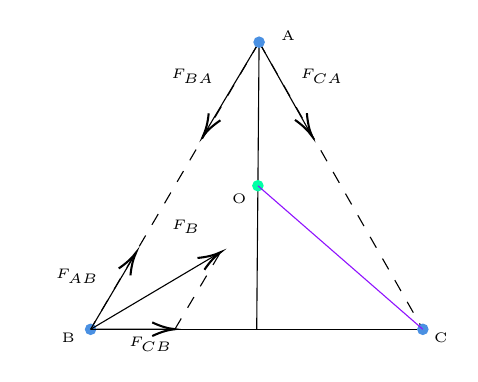
\begin{tikzpicture}[x=0.75pt,y=0.75pt,yscale=-1,xscale=1]
%uncomment if require: \path (0,300); %set diagram left start at 0, and has height of 300

%Straight Lines [id:da7411767697224816] 
\draw    (100,102) ;
%Straight Lines [id:da35334013949437937] 
\draw    (130.05,191.39) -- (290.12,191.39) ;
%Straight Lines [id:da8337888464734036] 
\draw    (211.23,53.05) -- (210.08,191.39) ;
%Straight Lines [id:da37892752623854364] 
\draw    (211.23,53.05) -- (185.19,96.68) ;
\draw [shift={(184.17,98.4)}, rotate = 300.82] [color={rgb, 255:red, 0; green, 0; blue, 0 }  ][line width=0.75]    (10.93,-3.29) .. controls (6.95,-1.4) and (3.31,-0.3) .. (0,0) .. controls (3.31,0.3) and (6.95,1.4) .. (10.93,3.29)   ;
%Straight Lines [id:da23461063513640812] 
\draw  [dash pattern={on 4.5pt off 4.5pt}]  (211.23,53.05) -- (130.05,191.39) ;
%Straight Lines [id:da4163775253760995] 
\draw  [dash pattern={on 4.5pt off 4.5pt}]  (211.23,53.05) -- (290.12,191.39) ;
%Straight Lines [id:da14314395431520932] 
\draw    (211.23,53.05) -- (235.78,96.66) ;
\draw [shift={(236.76,98.4)}, rotate = 240.62] [color={rgb, 255:red, 0; green, 0; blue, 0 }  ][line width=0.75]    (10.93,-3.29) .. controls (6.95,-1.4) and (3.31,-0.3) .. (0,0) .. controls (3.31,0.3) and (6.95,1.4) .. (10.93,3.29)   ;
%Shape: Circle [id:dp27435800391771203] 
\draw  [color={rgb, 255:red, 74; green, 144; blue, 226 }  ,draw opacity=1 ][fill={rgb, 255:red, 74; green, 144; blue, 226 }  ,fill opacity=1 ] (213.73,53.05) .. controls (213.73,51.67) and (212.61,50.55) .. (211.23,50.55) .. controls (209.85,50.55) and (208.73,51.67) .. (208.73,53.05) .. controls (208.73,54.43) and (209.85,55.55) .. (211.23,55.55) .. controls (212.61,55.55) and (213.73,54.43) .. (213.73,53.05) -- cycle ;
%Shape: Circle [id:dp355067680258665] 
\draw  [color={rgb, 255:red, 74; green, 144; blue, 226 }  ,draw opacity=1 ][fill={rgb, 255:red, 74; green, 144; blue, 226 }  ,fill opacity=1 ] (132.55,191.39) .. controls (132.55,190.01) and (131.43,188.89) .. (130.05,188.89) .. controls (128.67,188.89) and (127.55,190.01) .. (127.55,191.39) .. controls (127.55,192.77) and (128.67,193.89) .. (130.05,193.89) .. controls (131.43,193.89) and (132.55,192.77) .. (132.55,191.39) -- cycle ;
%Shape: Circle [id:dp8731378911211072] 
\draw  [color={rgb, 255:red, 74; green, 144; blue, 226 }  ,draw opacity=1 ][fill={rgb, 255:red, 74; green, 144; blue, 226 }  ,fill opacity=1 ] (292.62,191.39) .. controls (292.62,190.01) and (291.5,188.89) .. (290.12,188.89) .. controls (288.74,188.89) and (287.62,190.01) .. (287.62,191.39) .. controls (287.62,192.77) and (288.74,193.89) .. (290.12,193.89) .. controls (291.5,193.89) and (292.62,192.77) .. (292.62,191.39) -- cycle ;
%Shape: Circle [id:dp08553461642771443] 
\draw  [color={rgb, 255:red, 0; green, 255; blue, 165 }  ,draw opacity=1 ][fill={rgb, 255:red, 0; green, 255; blue, 165 }  ,fill opacity=1 ] (213.15,122.22) .. controls (213.15,120.84) and (212.04,119.72) .. (210.65,119.72) .. controls (209.27,119.72) and (208.15,120.84) .. (208.15,122.22) .. controls (208.15,123.6) and (209.27,124.72) .. (210.65,124.72) .. controls (212.04,124.72) and (213.15,123.6) .. (213.15,122.22) -- cycle ;
%Straight Lines [id:da7509716289501367] 
\draw [color={rgb, 255:red, 144; green, 19; blue, 254 }  ,draw opacity=1 ]   (210.65,122.22) -- (290.12,191.39) ;
%Straight Lines [id:da6715627766530636] 
\draw    (130.05,191.39) -- (168.67,191.34) ;
\draw [shift={(170.67,191.33)}, rotate = 179.92] [color={rgb, 255:red, 0; green, 0; blue, 0 }  ][line width=0.75]    (10.93,-3.29) .. controls (6.95,-1.4) and (3.31,-0.3) .. (0,0) .. controls (3.31,0.3) and (6.95,1.4) .. (10.93,3.29)   ;
%Straight Lines [id:da8234752419975047] 
\draw    (130.05,191.39) -- (150.98,156.05) ;
\draw [shift={(152,154.33)}, rotate = 120.64] [color={rgb, 255:red, 0; green, 0; blue, 0 }  ][line width=0.75]    (10.93,-3.29) .. controls (6.95,-1.4) and (3.31,-0.3) .. (0,0) .. controls (3.31,0.3) and (6.95,1.4) .. (10.93,3.29)   ;
%Straight Lines [id:da371469419005255] 
\draw  [dash pattern={on 4.5pt off 4.5pt}]  (170.67,191.33) -- (192.62,154.27) ;
%Straight Lines [id:da13561111516549063] 
\draw    (130.05,191.39) -- (190.9,155.29) ;
\draw [shift={(192.62,154.27)}, rotate = 149.32] [color={rgb, 255:red, 0; green, 0; blue, 0 }  ][line width=0.75]    (10.93,-3.29) .. controls (6.95,-1.4) and (3.31,-0.3) .. (0,0) .. controls (3.31,0.3) and (6.95,1.4) .. (10.93,3.29)   ;

% Text Node
\draw (220.67,46.33) node [anchor=north west][inner sep=0.75pt]  [font=\tiny] [align=left] {A};
% Text Node
\draw (115,192) node [anchor=north west][inner sep=0.75pt]  [font=\tiny] [align=left] {B};
% Text Node
\draw (294.33,192) node [anchor=north west][inner sep=0.75pt]  [font=\tiny] [align=left] {C};
% Text Node
\draw (197,125) node [anchor=north west][inner sep=0.75pt]  [font=\tiny] [align=left] {O};
% Text Node
\draw (167.67,64.67) node [anchor=north west][inner sep=0.75pt]  [font=\tiny] [align=left] {$\displaystyle F_{BA}$};
% Text Node
\draw (230,64.67) node [anchor=north west][inner sep=0.75pt]  [font=\tiny] [align=left] {$\displaystyle F_{CA}$};
% Text Node
\draw (112,161) node [anchor=north west][inner sep=0.75pt]  [font=\tiny] [align=left] {$\displaystyle F_{AB}$};
% Text Node
\draw (147.33,194) node [anchor=north west][inner sep=0.75pt]  [font=\tiny] [align=left] {$\displaystyle F_{CB}$};
% Text Node
\draw (168,137.33) node [anchor=north west][inner sep=0.75pt]  [font=\tiny] [align=left] {$\displaystyle F_{B}$};
\end{tikzpicture}

\end{center}
\end{minipage}
~\\

(3) B、C质心在BC中点,等效质量为$2m$,故三星系统质心在A与BC中点的连线的中点(O点)上,故由几何关系
$$R_C^2 = (\frac{1}{2} \cdot \frac{\sqrt{3}}{2} a)^2+(\frac{a}{2})^2$$
解得$R_C = \frac{\sqrt{7}}{4} a$
~\\

(4) 由对称性
$$F_C = F_B = \frac{\sqrt{7}G m^2}{a^2} = m \omega ^2 R_C$$
故$T=\frac{2 \pi}{\omega}=\pi \sqrt{\frac{a^3}{G m}}$

\end{ep}

若我们将系统看为整体,由动量定理,当且仅当这个整体受到外力时,系统总动量改变,因此有

\begin{theo}{系统动量定理}{}
对于一个质点系而言,只有合外力才会导致系统总动量发生变化,内力不影响系统总动量。
\end{theo}

\subsection{质心系\quad \dag \protect \footnote{带“\dag”号的章节在高考中用处较少,可选择阅读此章节部分内容}}

若我们选取系统的质心为参考点建立参考系,则我们称此参考系为\textbf{质心系}(记为CM系\footnote{CM为Center of Mass的缩写,意为“质心”})。

\begin{defi}[label=zxxsd]{质心系速度}{}
根据前文\defiref{zxdy},将式子两端对时间求导,可得质心系的速度

$$v_{cx} = \frac{\sum m_i v_{ix}}{\sum m_i} ,\quad v_{cy} = \frac{\sum m_i v_{iy}}{\sum m_i}$$
\end{defi}

在质心系中,有如下性质

\begin{theo}[label=zxxxtdl]{质心系系统动量}{}
在质心系中,质心速度为$0$,则根据\theoref{zxyxtzdl},系统总动量为$0$,即\textbf{质心系下系统的总动量为零}。写成矢量式为

\begin{equation}
\begin{aligned}
\sum m_i \cdot \vec{v_{ci}} = 0
\end{aligned}
\label{e_zxxdl}
\end{equation}

其中$\vec{v_{ci}}$为第$i$个物体在质心系中速度。
\end{theo}

\subsection{质心系动能定理 \quad \dag}

如果系统只做平动,系统中质点各个部分的速度完全相同,则物体可视为质点,动能当然可以由质心速度来计算。但当系统中质点有相对质心的运动时,则系统动能应由柯尼希(König)定理计算

\begin{theo}[label=knxdl]{柯尼希定理}{}
若系统中有$n$个质点,质点质量和相对质心速度分别为$m_1$、$v_{c1}$,$m_2$、$v_{c2}$……$m_n$、$v_{cn}$,则体系总动能为

$$E_{tot}=\frac{1}{2} m_{tot} v_c^2 + \sum \frac{1}{2} m_i v_{ci}^2$$

其中$m_{tot} = \sum m_i$为系统总质量,$v_c$为质心速度。记$\frac{1}{2} m_{tot} v_c^2$为质心动能,$\sum \frac{1}{2} m_i v_{ci}^2$为相对质心动能。即\textbf{系统总动能等于质心动能加上其他质点相对质心动能}。
\end{theo}

\begin{mk}{易错提醒}{}
根据柯尼希定理,由于系统总动能包含相对质心的动能这一项,故\textbf{不可以用质心速度变化来计算动能的变化量}。
\end{mk}

柯尼希定理证明如下:

在地面参考系中,质心速度为$\vec{v_c}$,第$i$个相对质心速度为$\vec{v_{ci}}$,根据前文速\secref{s_sdql},第$i$个质点相对地面速度为

$$\vec{v_i} = \vec{v_c} + \vec{v_{ci}}$$

则总动能

\begin{subequations}
\begin{align*}
E_{tot} &= \sum \frac{1}{2} m_i \tikzmarknode{v}{ \highlight{red}{$ \vec{v_i}^2 $} }\\
&= \sum \frac{1}{2} m_i \vec{v_c}^2 + \sum \frac{1}{2} m_i \vec{v_{ci}}^2 + \vec{v_i} \cdot \tikzmarknode{vci}{ \highlight{blue}{$ \sum m_i \vec{v_{ci}} $} } \\
&= \frac{1}{2} m_{tot} v_c^2 + \sum \frac{1}{2} m_i v_{ci}^2
\end{align*}
\end{subequations}

\begin{tikzpicture}[overlay,remember picture,>=stealth,nodes={align=left,inner ysep=1pt},<-]

\path (v.east) ++ (2em,0) node[anchor=west] (scalep){\highlight{red}{$ \vec{v_i}^2 = (\vec{v_c} + \vec{v_{ci}})^2 = \vec{v_c}^2 + \vec{v_{ci}}^2 + 2 \vec{v_c} \cdot \vec{v_{ci}} $}};
\draw [color=red!87](v.east) -- ([xshift=0.3ex,color=red]scalep.west);

\path (vci.south) ++ (2em,-3em) node[anchor=north] (scalep2){\highlight{blue}{根据\theoref{zxxxtdl},此项恒等于$0$}};
\draw [color=blue!87](vci.south) -- ([yshift=-0.3ex,color=blue]scalep2.north);

\end{tikzpicture}


证毕,QED。 

我们可以用此定理很快地得到完全非弹性碰撞损失能量公式。若两球发生完全非弹性碰撞,记两球质量和初速分别为$m_1$、$v_1$,$m_2$、$v_2$。则根据\defiref{zxxsd},可得

$$v_c = \frac{m_1 v_1 + m_2 v_2}{m_1+m_2}$$

两球相对质心速度分别为

$$v_{c1} = v_1 - v_c ,\quad v_{c2} = v_2 - v_c$$

由于系统动量守恒,故系统动量保持不变,质心动量保持不变,根据$p^2 = 2 m E_k$知质心动能保持不变。那么当相对质心速度均为$0$时,相对质心动能为$0$,此时系统总动能最小,两球共速(均为质心速度),能量损失最大。那么此时损失的能量

\begin{subequations}
\begin{align*}
\Delta E &= \frac{1}{2} m_1 v_{c1}^2 + \frac{1}{2} m_2 v_{c2}^2 \\
&= \frac{1}{2} \mu (v_2 - v_1)^2 \\
&= \frac{1}{2} \mu v_{in}^2
\end{align*}
\end{subequations}

即完全非弹性碰撞的能量损失公式。故有如下定理

\begin{theo}{碰撞中能量损失最值}{}
在两物体碰撞中,当碰撞为完全非弹性碰撞时,系统能量损失最大,为

$$\Delta E_{max} = \frac{1}{2} \mu v_{in}^2$$

其中$\mu=\frac{m_1 m_2}{m_1 + m_2}$为约化质量(约化质量定义见\secref{s_yhzl}),$v_{in}$为两球相对接近速度。
\end{theo}

%\section{等效碰撞}

%\subsection{等效完全非弹性碰撞}

%\subsection{等效完全弹性碰撞}

\section{恢复系数}

\subsection{定义与基本性质}

\begin{center}
\begin{tikzpicture}[x=0.75pt,y=0.75pt,yscale=-0.7,xscale=0.7]
%uncomment if require: \path (0,300); %set diagram left start at 0, and has height of 300

%Straight Lines [id:da09119880335817876] 
\draw    (170,80) -- (330,80) ;
%Straight Lines [id:da28100570617938536] 
\draw    (330,80) -- (330,250) ;
%Straight Lines [id:da7612411853487444] 
\draw    (323.33,222.33) -- (352,271.33) ;
%Straight Lines [id:da14847117572034363] 
\draw  [dash pattern={on 4.5pt off 4.5pt}]  (170,80) -- (330.67,232.67) ;
%Straight Lines [id:da030994288618529486] 
\draw    (328.67,231) -- (357.33,231) ;
% Plotting does not support converting to Tikz

% Text Node
\draw (193.67,89) node [anchor=north west][inner sep=0.75pt]  [font=\tiny] [align=left] {$\displaystyle \theta _{r}$};
% Text Node
\draw (339.67,234.67) node [anchor=north west][inner sep=0.75pt]  [font=\tiny] [align=left] {$\displaystyle \theta _{v}$};


\end{tikzpicture}

\end{center}

对于两个物体的碰撞过程,假设两物体质量为$m_1$、$m_2$初态时速度分别为$v_1$、$v_2$(以向右为正方向),末态时为$v_1^{\prime}$、$v_2^{\prime}$

\begin{defi}{恢复系数}{}
记两个物体接近时相对速度(接近速度)$\Delta v_{in} = v_1-v_2$,分离时相对速度(分离速度)$\Delta v_{out} = v_2^{\prime}-v_1^{\prime}$,则定义恢复系数

$$e = \frac{\Delta v_{out}}{\Delta v_{in}}$$

即恢复系数等于接近速度除以分离速度。
\end{defi}

现我们探讨不同情况下的恢复系数:

对于完全非弹性碰撞,碰撞后两物体共速,即分离速度$\Delta v_{out} = 0$,故此时恢复系数$e=0$。

对于完全弹性碰撞,碰撞过程满足能量守恒和动量守恒,故有
\begin{subequations}
\begin{align}
\label{e_eq1}
\frac{1}{2} m_1 v_1^2 + \frac{1}{2} m_2 v_2^2 &= \frac{1}{2} m_1 {v_1^{\prime}}^2 + \frac{1}{2} m_2 {v_2^{\prime}}^2 \\
\label{e_eq2}
m_1 v_1 + m_2 v_2 &= m_1 v_1^{\prime} + m_2 v_2^{\prime} 
\end{align}
\end{subequations}

化简式\eqref{e_eq1},移项,展开,得
\begin{equation}
\begin{aligned}
m_1 (v_1 + v_1^{\prime})(v_1 - v_1^{\prime}) = m_2 (v_2 + v_2^{\prime})(v_2^{\prime} - v_2)  
\end{aligned}
\label{e_eq3}
\end{equation}

将式\eqref{e_eq3}除以移项后的式\eqref{e_eq2},得$v_1 + v_1^{\prime} = v_2 + v_2^{\prime}$,即此时$e=1$。

\begin{theo}{完全弹性碰撞恢复系数}{}
在完全弹性碰撞中,恢复系数$e=1$,即\textbf{接近速度等于分离速度}
\end{theo}

对于非完全弹性碰撞,可以证明$0 < e <1$。

综上,我们可以用恢复系数表征不同碰撞类型,即:

\begin{itemize}
	\item 完全非弹性碰撞:$e = 0$
	\item 非完全弹性碰撞:$0 < e < 1$
	\item 完全弹性碰撞:$e = 1$
\end{itemize}

\subsection{完全弹性碰撞速度关系}

对于完全弹性碰撞,恢复系数$e=1$,即$v_1 + v_1^{\prime} = v_2 + v_2^{\prime}$,将其与动量守恒联立$m_1 v_1 + m_2 v_2 = m_1 v_1^{\prime} + m_2 v_2^{\prime}$,两个方程求解未知数,故有

\begin{theo}{完全弹性碰撞速度关系}{}
对于两个物体的碰撞过程,假设两物体质量为$m_1$、$m_2$初态时速度分别为$v_1$、$v_2$,末态时为$v_1^{\prime}$、$v_2^{\prime}$,则有

$$v_1^{\prime} = \frac{m_1 - m_2}{m_1 + m_2} v_1 + \frac{2 m_2}{m_1 + m_2} v_2 = 2 v_c - v_1$$
$$v_2^{\prime} = \frac{m_2 - m_1}{m_1 + m_2} v_2 + \frac{2 m_1}{m_1 + m_2} v_1 = 2 v_c - v_2$$

其中$v_c = \frac{m_1 v_1 + m_2 v_2}{m_1+m_2}$为质心速度(即完全非弹性碰撞后速度)。
\end{theo}

\subsection{恢复系数与能量关系}

从前文中我们可以得知,对于完全弹性碰撞,恢复系数$e=1$,$e=1$与能量守恒方程等价,可以借此简化完全弹性碰撞的公式推导。这一性质还可以在如下题目中将较复杂的能量计算转换为相对速度的计算,大大简化计算量。

\begin{ep}{练习题}{}
两球A、B在光滑水平线上沿同一直线,同一方向运动,$m_A = 1kg$,$m_B = 2kg$,$v_A = 6m/s$,$v_B = 2m/s$。当球A追上球B并发生碰撞后,两球A、B的速度可能是(取碰撞前两球运动方向为正)

A.$v_A^{\prime} = 5m/s$,$v_B^{\prime} = 2.5m/s$ \quad B.$v_A^{\prime} = 2m/s$,$v_B^{\prime} = 4m/s$

C.$v_A^{\prime} = -4m/s$,$v_B^{\prime} = 7m/s$ \quad D.$v_A^{\prime} = 7m/s$,$v_B^{\prime} = 1.5m/s$
~\\

对于上面四个选项,其动量均为$10kg \cdot m/s$,故只能从能量和两球速度判断。
由于碰撞后不可能出现球A、球B速度同向且A速度大于B速度的情况,故选项AD错误。由前文得知,分离速度不大于接近速度。接近速度$v_{in}=4m/s$,对于B,分离速度$v_{out} = 2m/s$;对于C,分离速度$v_{out} = 11m/s$,大于接近速度。故B对,C错。综上,选B。
\end{ep}

更进一步的,我们还可以求出$e$与体系因碰撞损失能量$\Delta E$的关系。

\begin{equation}
\begin{aligned}
\Delta E &= \frac{1}{2} m_1 {v_1^{\prime}}^2 + \frac{1}{2} m_2 {v_2^{\prime}}^2 - \frac{1}{2} m_1 v_1^2 - \frac{1}{2} m_2 v_2^2 \\
0 &= m_1 v_1^{\prime} + m_2 v_2^{\prime} - m_1 v_1 - m_2 v_2 \\
e &= \frac{v_2^{\prime} - v_1^{\prime}}{v_1 - v_2}
\end{aligned}
\label{e_eq4}
\end{equation}

联立式\eqref{e_eq4},解得碰撞损失能量$\Delta E$与$e$的关系,如下

\begin{theo}{恢复系数与损失能量关系}{}
碰撞损失能量$\Delta E$与$e$满足如下关系
$$\Delta E = (1 - e^2) \cdot \frac{1}{2} \mu v_{in}^2 = (1 - e^2) \Delta E_{max}$$
其中$\mu=\frac{m_1 m_2}{m_1 + m_2}$为约化质量(约化质量定义见\secref{s_yhzl}),接近速度$v_{in} = v_2 - v_1$
\end{theo}

\begin{mk}{思考}{}
此定理可以使用质心动能定理简便证明,试用质心动能定理证明该定理。
\end{mk}

这个定理可以应用在如下模型之中

\begin{ep}{自编题}{}
现有一质量为$M=0.9kg$的物体静止在光滑水平面上,一质量为$m=0.1kg$的子弹以速度$v=100m/s$打穿木块(忽略重力对子弹轨迹的偏移),穿出木块后木块速度为$v_M = 1m/s$,试求子弹穿出木块后子弹速度$v_m$及整个系统发热$Q$
~\\

先用动量守恒求出$v_m$:

$$m v = m v_m + M v_M$$

解的$v_m = 91m/s$。分离速度$v_{out} =  91 - 1 = 90m/s$,接近速度$v_{in} = 100m/s$因此$e = \frac{90}{100} = 0.9$,套用结论,得

$$\Delta E = (1 - 0.9^2) \cdot \frac{1}{2} \frac{0.9 \times 0.1}{0.9 + 0.1} \cdot 100^2 = 85.5J$$
\end{ep}

当然,以上模型还可以扩展到其他情况,如对于穿出过程中子弹得到加速,系统总机械能增加的情况,此时按照结论计算得到的$\Delta E$为负值,即损失了负数的能量,即其绝对值为系统总机械能增加值。但此情况出现很少,在此不再叙述。

\section{反冲运动能量变化}

设在地面系中,有两个物体$A$和$B$,质量分别为$m_A$、$m_B$,开始时两物体粘连在一起在地面保持静止。在某一时刻时,$A$、$B$之间的炸药爆炸,将$A$、$B$炸分离。炸药释放的能量为$\Delta E$。根据动量守恒,分离后$A$、$B$的动量相同,记为$\Delta p$。则由能量守恒分别有:

$$\Delta E = \frac{\Delta p^2}{2 m_A} + \frac{\Delta p^2}{2 m_B}$$

根据前文定义,记$\mu = \frac{m_A m_B}{m_A + m_B}$为约化质量(约化质量定义见\secref{s_yhzl}),因此上式可化简为

$$\Delta p^2 = 2 \mu \Delta E$$

上面的式子可以推广到更广泛的情况。设在地面系中,有两个物体$A$和$B$,质量分别为$m_A$、$m_B$,开始时两物体粘连在一起,以速度$v_0$共同运动。在某一时刻时,$A$、$B$之间的炸药爆炸,将$A$、$B$炸分离。炸药释放的能量为$\Delta E$。设分离后物体$A$、$B$的速度为$v_A$、$v_B$。由于动量守恒可得$A$、$B$动量改变量相同,记为$\Delta p$。故

$$\Delta p = m_A (v_0 - v_A) = m_B (v_B - v_0)$$

$$(v_0 - v_A)^2 = \frac{\Delta p^2}{m_A^2} ,\quad (v_B - v_0)^2 = \frac{\Delta p^2}{m_B^2}$$

由\theoref{knxdl}可知,爆炸前由于两物体均没有相对质心运动,故系统动能为

$$E = \frac{1}{2} (m_A + m_B) v_0^2$$

爆炸后系统动能为

$$E^{\prime} = \frac{1}{2} (m_A + m_B) v_0^2 + \frac{1}{2} m_A (v_0 - v_A)^2 + \frac{1}{2} m_B (v_B - v_0)^2$$

故

$$\Delta E = E^{\prime} - E = \frac{1}{2} m_A (v_0 - v_A)^2 + \frac{1}{2} m_B (v_B - v_0)^2$$

将前文式子带入上式,化简,记$\mu = \frac{m_A m_B}{m_A + m_B}$为约化质量,得

$$\Delta p^2 = 2 \mu \Delta E$$

\begin{theo}{反冲运动能量变化}{}
若有两个物体$A$和$B$,质量分别为$m_A$、$m_B$,\textbf{初始时两物体共速},之后由于其他形式能量转化两物体分离,能量增加为$\Delta E$,则两物体动量改变量$\Delta p$满足

$$\Delta p^2 = 2 \mu \Delta E$$

其中$\mu = \frac{m_A m_B}{m_A + m_B}$为约化质量(约化质量定义见\secref{s_yhzl})。
\end{theo}

\begin{mk}{思考}{}
此定理一个重要的前提是初始时两物体共速。试假设初始时两物体不共速,尝试按照上述步骤进行推导,并说明若初始时两物体不共速时此定理不成立的原因。
\end{mk}

%# -*- coding: utf-8-unix -*-
%%==================================================
\tikzset{every picture/.style={line width=0.75pt}} %set default line width to 0.75pt        

\chapter{电磁学}

\begin{mk}{本章符号约定}{}
在电学中,能量,电场,电势能,电动势在高中课本中均用符号$E$来表示,在遇到综合性问题时可能会出现混淆,在未说明的情况下,按照如下符号规则进行区分:

\begin{itemize}
\item 能量使用符号$E_{k0}$来表示,英文下标代表能量类型($k$为动能,$p$为势能等),以数学作为下标
\item 电场使用符号$E_a$来表示,以单独的小写英文作为下标
\item 电势能使用$q \Delta \varphi$或者$E_{p0}$来表示(势能只有电势能时)
\item 电动势使用英文E的花体$\ms E$表示\footnote{此处电动势作此约定一方面为了便于区分,另一方面为了跟大学教材的符号约定相同}
\end{itemize}
\end{mk}

\section{电源输出功率性质}
\label{s_wdlzdgl}

现有一个电动势为$\ms E$、内阻为$r$的电源,跟一个电阻为$R$的可变电阻串联,现推导电源输出功率功率与电阻阻值关系。

\begin{subequations}
\begin{align*}
I &= \frac{\ms E}{r + R} \\
P &= I^2 R = \frac{\ms E^2 R}{(r + R)^2}
\end{align*}
\end{subequations}

上面$P = \frac{\ms E^2 R}{(r + R)^2}$中$P$关于$R$的函数图像如下图所示(取$\ms E = 1$、$r = 1$)

\begin{figure}[htbp]
\centering
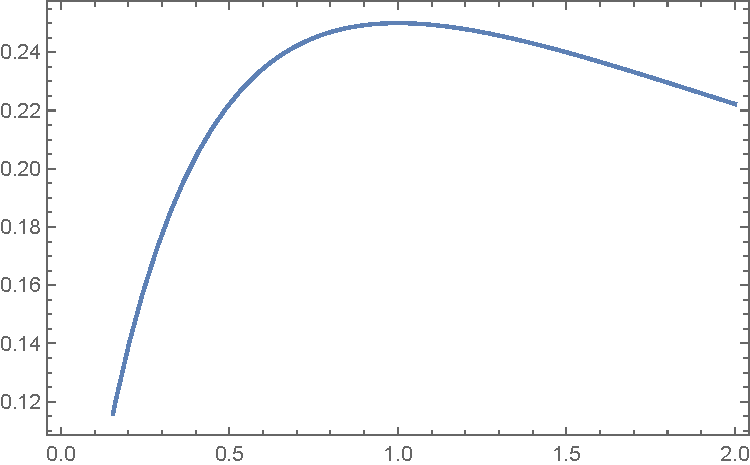
\includegraphics[width=0.5\textwidth]{pic_eled/zdgl_p1.pdf}
\end{figure}

可见存在$R$,使得$P$取得最大值。对$P = \frac{\ms E^2 R}{(r + R)^2}$求导,得

$$P^{\prime}(R) = \frac{\ms E^2}{(r+R)^2}-\frac{2 R \ms E^2}{(r+R)^3} = \frac{\ms E^2 (r-R)}{(r+R)^3}$$

可见,当$R=r$时,$P^{\prime} = 0$,此时$P$最大。由图可知,$R$越接近$r$,电源输出功率$P$越大。并且,我们可以从$P$中反解出$R$,化简得到

$$P R^2 + (2 r P - \ms E^2)R + P r^2 = 0$$

由韦达(Vieta)定理:$R$的两根满足$R_1 R_2 = r^2$,即$r = \sqrt{R_1 R_2}$,故

\begin{theo}{电源输出功率性质}{}
当外电路总电阻$R$等于电源内阻$r$时,电源输出功率最大;

外电路总电阻$R$越接近电源内阻$r$,电源输出功率越大;

若两个不同的外电路总电阻对应同一电源输出功率,则这两个外电路总电阻满足$r = \sqrt{R_1 R_2}$。
\end{theo}

\section{等效源}
\label{s_dxy}

\subsection{电压源与电流源}

在高中中,\textbf{一个没有电阻的理想电源,其输出电压不随着外电路改变而改变,始终保持一个恒定值,我们称此理想电源为理想电压源}。

同样的,根据如上进行类比,\textbf{若有这么一个理想电源,其输出的电流输出电压不随着外电路改变而改变,始终保持一个恒定值,我们称此理想电源为理想电流源}。

但在现实生活中,由于电源存在内阻,其输出电压或者电流会随着外电路变化而变化,故不存在完全理想的电源。此时我们可以将理想电压源串联一个电阻组成包含内阻的电压源,将理想电流源并联一个电阻组成包含内阻的电流源,即对于包含内阻的电压源与电流源,其等效的电路图如下图所示

\begin{center}


\begin{tikzpicture}[x=0.75pt,y=0.75pt,yscale=-1.4,xscale=1.4]
%uncomment if require: \path (0,300); %set diagram left start at 0, and has height of 300

%Shape: Resistor [id:dp7232411406538839] 
\draw   (155.4,185) -- (174.6,185) -- (174.6,195) -- (155.4,195) -- (155.4,185) -- cycle (150,190) -- (155.4,190) (174.6,190) -- (180,190) ;
%Shape: Battery [id:dp6693718019533714] 
\draw   (120,190) -- (133.5,190) (136.5,179.36) -- (136.5,200.64) (136.5,190) -- (150,190) (132.3,184.68) -- (133.5,184.68) -- (133.5,195.32) -- (132.3,195.32) -- (132.3,184.68) -- cycle ;
%Straight Lines [id:da16042882813115766] 
\draw    (100,140) -- (100,190) ;
%Straight Lines [id:da9402822543750411] 
\draw    (190,140) -- (190,190) ;
%Straight Lines [id:da12067780236857573] 
\draw    (100,190) -- (120,190) ;
%Straight Lines [id:da32759114986333504] 
\draw    (180,190) -- (190,190) ;
%Shape: Resistor [id:dp12513559180930134] 
\draw   (295.4,165) -- (314.6,165) -- (314.6,175) -- (295.4,175) -- (295.4,165) -- cycle (290,170) -- (295.4,170) (314.6,170) -- (320,170) ;
%Straight Lines [id:da8542668820839858] 
\draw    (260,139.36) -- (260,189.36) ;
%Straight Lines [id:da980396874368167] 
\draw    (350,139.36) -- (350,189.36) ;
%Straight Lines [id:da7073460320803453] 
\draw    (260,189.36) -- (290,189.5) ;
%Straight Lines [id:da37259186085045526] 
\draw    (324.6,189.5) -- (350,189.36) ;
%Shape: Output [id:dp7159850466470945] 
\draw   (298.65,189.5) .. controls (298.65,184.25) and (302.52,180) .. (307.3,180) .. controls (312.08,180) and (315.95,184.25) .. (315.95,189.5) .. controls (315.95,194.75) and (312.08,199) .. (307.3,199) .. controls (302.52,199) and (298.65,194.75) .. (298.65,189.5) -- cycle (290,189.5) -- (298.65,189.5) (324.6,189.5) -- (315.95,189.5) ;
%Straight Lines [id:da774504718728555] 
\draw    (290,170) -- (260,170) ;
%Straight Lines [id:da2518342963725635] 
\draw    (350,170) -- (320,170) ;
%Straight Lines [id:da6515640173772954] 
\draw    (298.65,189.5) -- (313.95,189.5) ;
\draw [shift={(315.95,189.5)}, rotate = 180] [color={rgb, 255:red, 0; green, 0; blue, 0 }  ][line width=0.75]    (10.93,-3.29) .. controls (6.95,-1.4) and (3.31,-0.3) .. (0,0) .. controls (3.31,0.3) and (6.95,1.4) .. (10.93,3.29)   ;
%Shape: Rectangle [id:dp025798222389296965] 
\draw  [dash pattern={on 4.5pt off 4.5pt}] (110,170) -- (180,170) -- (180,210) -- (110,210) -- cycle ;
%Shape: Rectangle [id:dp000655868679727778] 
\draw  [dash pattern={on 4.5pt off 4.5pt}] (254.6,150) -- (355,150) -- (355,210) -- (254.6,210) -- cycle ;

% Text Node
\draw (121,222) node [anchor=north west][inner sep=0.75pt]  [font=\tiny] [align=left] {电压源};
% Text Node
\draw (281,222) node [anchor=north west][inner sep=0.75pt]  [font=\tiny] [align=left] {电流源};
% Text Node
\draw (122,173.5) node [anchor=north west][inner sep=0.75pt]   [align=left] {$ $};
% Text Node
\draw (118,175) node [anchor=north west][inner sep=0.75pt]  [font=\tiny] [align=left] {$\displaystyle \ms E$};
% Text Node
\draw (148,175) node [anchor=north west][inner sep=0.75pt]  [font=\tiny] [align=left] {$\displaystyle r$};
% Text Node
\draw (288,155) node [anchor=north west][inner sep=0.75pt]  [font=\tiny] [align=left] {$\displaystyle r$};
% Text Node
\draw (281,174) node [anchor=north west][inner sep=0.75pt]  [font=\tiny] [align=left] {$\displaystyle I_{0}$};
\end{tikzpicture}

\end{center}

电压源中$\ms E$为电源电动势,$r$为电源内阻;电流源中$I_0$为理想电流源恒定输出电流,$r$为电源内阻。

\begin{mk}{符号约定}{}
如无一般说明,电源内阻会在电源外画出,即将电源电动势和内阻分开绘画
\end{mk}

\subsection{电压源与电流源间关系}
\label{dyydlygx}

电压源与电流源可以相互转化替代,记电压源电动势为$\ms E$,内阻为$r_{\ms E}$,电流源中理想电流源输出电流$I_0$,内阻$r_I$现粗略推导两个相互等效的电压源与电流源间关系:

\begin{itemize}
\item 当两个电源短路时,由短路电流相等得$\frac{\ms E}{r_{\ms E}} = I_0$
\item 当两个电源开路时,由开路电压相等得$I_0 r_I = \ms E$
\end{itemize}

由上面两个式子联立\footnote{这便是在绘制电压源和电流源内部等效示意图时不区分电压源电流源内阻统一用$r$的原因},解得$r = r_{\ms E} = r_{I}$、$\ms E = I_0 r $,故有

\begin{theo}{电压源与电流源间关系}{}
对于两个相互等效的电压源和电流源,满足
$$r = r_{\ms E} = r_{I} \quad \ms E = I_0 r$$
\end{theo}

\subsection{戴维宁定理与诺顿定理}

对于一个复杂的电路网络,我们总可以将某个电阻或者某段电路外的其他电路等效为一个电压源或电流源。现取如下电路:

\begin{center}

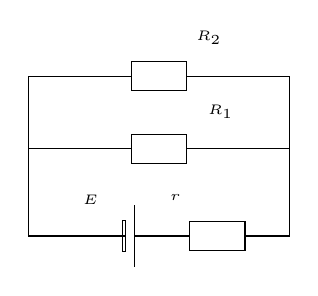
\begin{tikzpicture}[x=0.75pt,y=0.75pt,yscale=-1.4,xscale=1.4]
%uncomment if require: \path (0,300); %set diagram left start at 0, and has height of 300

%Shape: Resistor [id:dp514309969460313] 
\draw   (265.9,120) -- (285.1,120) -- (285.1,130) -- (265.9,130) -- (265.9,120) -- cycle (260.5,125) -- (265.9,125) (285.1,125) -- (290.5,125) ;
%Shape: Battery [id:dp2916012360245832] 
\draw   (230.5,125) -- (244,125) (247,114.36) -- (247,135.64) (247,125) -- (260.5,125) (242.8,119.68) -- (244,119.68) -- (244,130.32) -- (242.8,130.32) -- (242.8,119.68) -- cycle ;
%Straight Lines [id:da2734255254924993] 
\draw    (210.5,70) -- (210.5,125) ;
%Straight Lines [id:da8342089479991157] 
\draw    (300.5,70) -- (300.5,125) ;
%Straight Lines [id:da4571525926989708] 
\draw    (210.5,125) -- (230.5,125) ;
%Straight Lines [id:da08274074907134321] 
\draw    (290.5,125) -- (300.5,125) ;
%Shape: Resistor [id:dp8558892883342235] 
\draw   (245.9,90) -- (265.1,90) -- (265.1,100) -- (245.9,100) -- (245.9,90) -- cycle (240.5,95) -- (245.9,95) (265.1,95) -- (270.5,95) ;
%Straight Lines [id:da7537185022486395] 
\draw    (240.5,95) -- (210.5,95) ;
%Straight Lines [id:da8797643160506492] 
\draw    (300.5,95) -- (270.5,95) ;
%Shape: Resistor [id:dp5429151855494494] 
\draw   (245.9,65) -- (265.1,65) -- (265.1,75) -- (245.9,75) -- (245.9,65) -- cycle (240.5,70) -- (245.9,70) (265.1,70) -- (270.5,70) ;
%Straight Lines [id:da9804503401878168] 
\draw    (240.5,70) -- (210.5,70) ;
%Straight Lines [id:da5427185273385342] 
\draw    (300.5,70) -- (270.5,70) ;

% Text Node
\draw (232.5,108.5) node [anchor=north west][inner sep=0.75pt]   [align=left] {$ $};
% Text Node
\draw (228.5,110) node [anchor=north west][inner sep=0.75pt]  [font=\tiny] [align=left] {$\displaystyle \ms E$};
% Text Node
\draw (258.5,110) node [anchor=north west][inner sep=0.75pt]  [font=\tiny] [align=left] {$\displaystyle r$};
% Text Node
\draw (271.5,79) node [anchor=north west][inner sep=0.75pt]  [font=\tiny] [align=left] {$\displaystyle R_{1}$};
% Text Node
\draw (267.5,53.5) node [anchor=north west][inner sep=0.75pt]  [font=\tiny] [align=left] {$\displaystyle R_{2}$};


\end{tikzpicture}

\end{center}

如果我们想将除了$R_2$外的电路等效为一个电压源,则我们可以使用戴维宁\footnote{有些教材又称其为戴维南定理}(Thevenin)定理(又称等效电压源定理)

\begin{theo}[label=dwndl]{戴维宁定理}{}
对于一个二端有源电路网络,若电路中只有线性元件\footnote{这里线性元件一般指纯电阻,或稳定交流电下的电容和电感(他们在交流电下具有容抗和感抗,可等效为电阻(不考虑相位变化情况下),但在高中一般不要求分析具有容抗和感抗的交流电路,故一般情况下只需考虑纯电阻,对于下文诺顿定理同理},则我们可以将其等效为一个电压源,其\textbf{等效电动势等于两端的开路电压,等效内阻等于去除电动势后两端的电阻}。

这里“二端有源电路网络”中所指的“网络”泛指电路中其中一部分,“有源”指这部分电路中包含电源,“二端”指这段电路只有两个端口。对于下面的诺顿定理同理。
\end{theo}

对于上面的电路,以下标eq\footnote{equivalent的简写}代表等效的值,根据戴维南定理有

\begin{center}

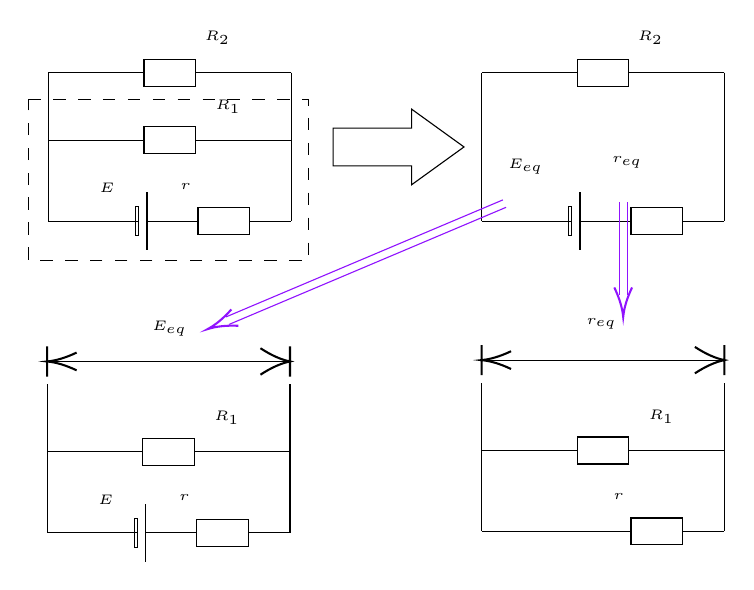
\begin{tikzpicture}[x=0.75pt,y=0.75pt,yscale=-1.3,xscale=1.3]
%uncomment if require: \path (0,300); %set diagram left start at 0, and has height of 300

%Shape: Resistor [id:dp7232411406538839] 
\draw   (245.9,100) -- (265.1,100) -- (265.1,110) -- (245.9,110) -- (245.9,100) -- cycle (240.5,105) -- (245.9,105) (265.1,105) -- (270.5,105) ;
%Shape: Battery [id:dp6693718019533714] 
\draw   (210.5,105) -- (224,105) (227,94.36) -- (227,115.64) (227,105) -- (240.5,105) (222.8,99.68) -- (224,99.68) -- (224,110.32) -- (222.8,110.32) -- (222.8,99.68) -- cycle ;
%Straight Lines [id:da16042882813115766] 
\draw    (190.5,50) -- (190.5,105) ;
%Straight Lines [id:da9402822543750411] 
\draw    (280.5,50) -- (280.5,105) ;
%Straight Lines [id:da12067780236857573] 
\draw    (190.5,105) -- (210.5,105) ;
%Straight Lines [id:da32759114986333504] 
\draw    (270.5,105) -- (280.5,105) ;
%Shape: Resistor [id:dp044708648259699446] 
\draw   (225.9,70) -- (245.1,70) -- (245.1,80) -- (225.9,80) -- (225.9,70) -- cycle (220.5,75) -- (225.9,75) (245.1,75) -- (250.5,75) ;
%Straight Lines [id:da8149590161538551] 
\draw    (220.5,75) -- (190.5,75) ;
%Straight Lines [id:da37292062821096206] 
\draw    (280.5,75) -- (250.5,75) ;
%Shape: Resistor [id:dp8915224058603441] 
\draw   (225.9,45) -- (245.1,45) -- (245.1,55) -- (225.9,55) -- (225.9,45) -- cycle (220.5,50) -- (225.9,50) (245.1,50) -- (250.5,50) ;
%Straight Lines [id:da8050738969027882] 
\draw    (220.5,50) -- (190.5,50) ;
%Straight Lines [id:da41847017454589475] 
\draw    (280.5,50) -- (250.5,50) ;
%Shape: Resistor [id:dp8946522623697388] 
\draw   (406.4,100) -- (425.6,100) -- (425.6,110) -- (406.4,110) -- (406.4,100) -- cycle (401,105) -- (406.4,105) (425.6,105) -- (431,105) ;
%Shape: Battery [id:dp4946459974897708] 
\draw   (371,105) -- (384.5,105) (387.5,94.36) -- (387.5,115.64) (387.5,105) -- (401,105) (383.3,99.68) -- (384.5,99.68) -- (384.5,110.32) -- (383.3,110.32) -- (383.3,99.68) -- cycle ;
%Straight Lines [id:da8491657091150393] 
\draw    (351,50) -- (351,105) ;
%Straight Lines [id:da8293033184283518] 
\draw    (441,50) -- (441,105) ;
%Straight Lines [id:da6903389383039646] 
\draw    (351,105) -- (371,105) ;
%Straight Lines [id:da4919692394445716] 
\draw    (431,105) -- (441,105) ;
%Shape: Resistor [id:dp9226843247374981] 
\draw   (386.4,45) -- (405.6,45) -- (405.6,55) -- (386.4,55) -- (386.4,45) -- cycle (381,50) -- (386.4,50) (405.6,50) -- (411,50) ;
%Straight Lines [id:da5240532491363821] 
\draw    (381,50) -- (351,50) ;
%Straight Lines [id:da8200773875832033] 
\draw    (441,50) -- (411,50) ;
%Right Arrow [id:dp12563132066413996] 
\draw   (296,70.5) -- (325.1,70.5) -- (325.1,63.5) -- (344.5,77.5) -- (325.1,91.5) -- (325.1,84.5) -- (296,84.5) -- cycle ;
%Shape: Rectangle [id:dp8119351522330263] 
\draw  [dash pattern={on 4.5pt off 4.5pt}] (183,60) -- (287,60) -- (287,119.5) -- (183,119.5) -- cycle ;
%Shape: Resistor [id:dp9181595801961024] 
\draw   (245.4,215.5) -- (264.6,215.5) -- (264.6,225.5) -- (245.4,225.5) -- (245.4,215.5) -- cycle (240,220.5) -- (245.4,220.5) (264.6,220.5) -- (270,220.5) ;
%Shape: Battery [id:dp8638451126944211] 
\draw   (210,220.5) -- (223.5,220.5) (226.5,209.86) -- (226.5,231.14) (226.5,220.5) -- (240,220.5) (222.3,215.18) -- (223.5,215.18) -- (223.5,225.82) -- (222.3,225.82) -- (222.3,215.18) -- cycle ;
%Straight Lines [id:da9493469917798139] 
\draw    (190,165.5) -- (190,220.5) ;
%Straight Lines [id:da9469350410050841] 
\draw    (280,165.5) -- (280,220.5) ;
%Straight Lines [id:da9707422227961422] 
\draw    (190,220.5) -- (210,220.5) ;
%Straight Lines [id:da47902505858245004] 
\draw    (270,220.5) -- (280,220.5) ;
%Shape: Resistor [id:dp44228410120226136] 
\draw   (225.4,185.5) -- (244.6,185.5) -- (244.6,195.5) -- (225.4,195.5) -- (225.4,185.5) -- cycle (220,190.5) -- (225.4,190.5) (244.6,190.5) -- (250,190.5) ;
%Straight Lines [id:da7513382191815712] 
\draw    (220,190.5) -- (190,190.5) ;
%Straight Lines [id:da4997577437287888] 
\draw    (280,190.5) -- (250,190.5) ;
%Straight Lines [id:da29586923725139136] 
\draw    (190,157) -- (280,157) ;
\draw [shift={(280,157)}, rotate = 180] [color={rgb, 255:red, 0; green, 0; blue, 0 }  ][line width=0.75]    (0,5.59) -- (0,-5.59)(10.93,-4.9) .. controls (6.95,-2.3) and (3.31,-0.67) .. (0,0) .. controls (3.31,0.67) and (6.95,2.3) .. (10.93,4.9)   ;
\draw [shift={(190,157)}, rotate = 0] [color={rgb, 255:red, 0; green, 0; blue, 0 }  ][line width=0.75]    (0,5.59) -- (0,-5.59)(10.93,-3.29) .. controls (6.95,-1.4) and (3.31,-0.3) .. (0,0) .. controls (3.31,0.3) and (6.95,1.4) .. (10.93,3.29)   ;
%Shape: Resistor [id:dp0668394417226108] 
\draw   (406.4,215) -- (425.6,215) -- (425.6,225) -- (406.4,225) -- (406.4,215) -- cycle (401,220) -- (406.4,220) (425.6,220) -- (431,220) ;
%Straight Lines [id:da585027680617425] 
\draw    (351,165) -- (351,220) ;
%Straight Lines [id:da24202593084033786] 
\draw    (441,165) -- (441,220) ;
%Straight Lines [id:da7950606810490672] 
\draw    (351,220) -- (401,220) ;
%Straight Lines [id:da9338085769888853] 
\draw    (431,220) -- (441,220) ;
%Shape: Resistor [id:dp9351098294796791] 
\draw   (386.4,185) -- (405.6,185) -- (405.6,195) -- (386.4,195) -- (386.4,185) -- cycle (381,190) -- (386.4,190) (405.6,190) -- (411,190) ;
%Straight Lines [id:da7426770619592475] 
\draw    (381,190) -- (351,190) ;
%Straight Lines [id:da4939519386694273] 
\draw    (441,190) -- (411,190) ;
%Straight Lines [id:da5374904022522706] 
\draw    (351,156.5) -- (441,156.5) ;
\draw [shift={(441,156.5)}, rotate = 180] [color={rgb, 255:red, 0; green, 0; blue, 0 }  ][line width=0.75]    (0,5.59) -- (0,-5.59)(10.93,-4.9) .. controls (6.95,-2.3) and (3.31,-0.67) .. (0,0) .. controls (3.31,0.67) and (6.95,2.3) .. (10.93,4.9)   ;
\draw [shift={(351,156.5)}, rotate = 0] [color={rgb, 255:red, 0; green, 0; blue, 0 }  ][line width=0.75]    (0,5.59) -- (0,-5.59)(10.93,-3.29) .. controls (6.95,-1.4) and (3.31,-0.3) .. (0,0) .. controls (3.31,0.3) and (6.95,1.4) .. (10.93,3.29)   ;
%Straight Lines [id:da48480372543600314] 
\draw [color={rgb, 255:red, 144; green, 19; blue, 254 }  ,draw opacity=1 ]   (360.08,99.88) -- (257.45,143.27)(358.92,97.12) -- (256.28,140.5) ;
\draw [shift={(249.5,145)}, rotate = 337.08] [color={rgb, 255:red, 144; green, 19; blue, 254 }  ,draw opacity=1 ][line width=0.75]    (10.93,-3.29) .. controls (6.95,-1.4) and (3.31,-0.3) .. (0,0) .. controls (3.31,0.3) and (6.95,1.4) .. (10.93,3.29)   ;
%Straight Lines [id:da6108098931367383] 
\draw [color={rgb, 255:red, 144; green, 19; blue, 254 }  ,draw opacity=1 ]   (405,98) -- (405,132.5)(402,98) -- (402,132.5) ;
\draw [shift={(403.5,140.5)}, rotate = 270] [color={rgb, 255:red, 144; green, 19; blue, 254 }  ,draw opacity=1 ][line width=0.75]    (10.93,-3.29) .. controls (6.95,-1.4) and (3.31,-0.3) .. (0,0) .. controls (3.31,0.3) and (6.95,1.4) .. (10.93,3.29)   ;

% Text Node
\draw (212.5,88.5) node [anchor=north west][inner sep=0.75pt]   [align=left] {$ $};
% Text Node
\draw (208.5,90) node [anchor=north west][inner sep=0.75pt]  [font=\tiny] [align=left] {$\displaystyle \ms E$};
% Text Node
\draw (238.5,90) node [anchor=north west][inner sep=0.75pt]  [font=\tiny] [align=left] {$\displaystyle r$};
% Text Node
\draw (251.5,59) node [anchor=north west][inner sep=0.75pt]  [font=\tiny] [align=left] {$\displaystyle R_{1}$};
% Text Node
\draw (247.5,33.5) node [anchor=north west][inner sep=0.75pt]  [font=\tiny] [align=left] {$\displaystyle R_{2}$};
% Text Node
\draw (373,88.5) node [anchor=north west][inner sep=0.75pt]   [align=left] {$ $};
% Text Node
\draw (360,81) node [anchor=north west][inner sep=0.75pt]  [font=\tiny] [align=left] {$\displaystyle \ms E_{eq}$};
% Text Node
\draw (398.5,80) node [anchor=north west][inner sep=0.75pt]  [font=\tiny] [align=left] {$\displaystyle r_{eq}$};
% Text Node
\draw (408,33.5) node [anchor=north west][inner sep=0.75pt]  [font=\tiny] [align=left] {$\displaystyle R_{2}$};
% Text Node
\draw (212,204) node [anchor=north west][inner sep=0.75pt]   [align=left] {$ $};
% Text Node
\draw (208,205.5) node [anchor=north west][inner sep=0.75pt]  [font=\tiny] [align=left] {$\displaystyle \ms E$};
% Text Node
\draw (238,205.5) node [anchor=north west][inner sep=0.75pt]  [font=\tiny] [align=left] {$\displaystyle r$};
% Text Node
\draw (251,174.5) node [anchor=north west][inner sep=0.75pt]  [font=\tiny] [align=left] {$\displaystyle R_{1}$};
% Text Node
\draw (228,141) node [anchor=north west][inner sep=0.75pt]  [font=\tiny] [align=left] {$\displaystyle \ms E_{eq}$};
% Text Node
\draw (399,205) node [anchor=north west][inner sep=0.75pt]  [font=\tiny] [align=left] {$\displaystyle r$};
% Text Node
\draw (412,174) node [anchor=north west][inner sep=0.75pt]  [font=\tiny] [align=left] {$\displaystyle R_{1}$};
% Text Node
\draw (389,140) node [anchor=north west][inner sep=0.75pt]  [font=\tiny] [align=left] {$\displaystyle r_{eq}$};


\end{tikzpicture}

\end{center}

\begin{subequations}
\begin{align*}
\ms E_{eq} &= \frac{\ms E R_1}{r + R_1} \\
r_{eq} &= \frac{r R_1}{r + R_1}
\end{align*}
\end{subequations}

同理,如果我们想将除了$R_2$外的电路等效为一个电压源,则我们可以使用诺顿(Norton)定理(又称等效电流源定理)

\begin{theo}{诺顿定理}{}
对于一个二端有源电路网络,若电路中只有线性元件,则我们可以将其等效为一个电流源,其\textbf{等效理想电流源电流等于两端短路时电流,等效内阻等于去除电动势后两端的电阻}。
\end{theo}

对于上面的电路,以下标eq代表等效的值,根据诺顿定理有

\begin{center}
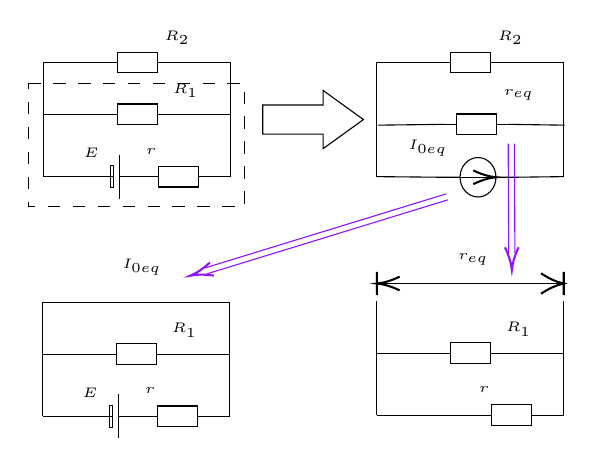
\begin{tikzpicture}[x=0.75pt,y=0.75pt,yscale=-1,xscale=1]
%uncomment if require: \path (0,300); %set diagram left start at 0, and has height of 300

%Shape: Resistor [id:dp7232411406538839] 
\draw   (245.9,100) -- (265.1,100) -- (265.1,110) -- (245.9,110) -- (245.9,100) -- cycle (240.5,105) -- (245.9,105) (265.1,105) -- (270.5,105) ;
%Shape: Battery [id:dp6693718019533714] 
\draw   (210.5,105) -- (224,105) (227,94.36) -- (227,115.64) (227,105) -- (240.5,105) (222.8,99.68) -- (224,99.68) -- (224,110.32) -- (222.8,110.32) -- (222.8,99.68) -- cycle ;
%Straight Lines [id:da16042882813115766] 
\draw    (190.5,50) -- (190.5,105) ;
%Straight Lines [id:da9402822543750411] 
\draw    (280.5,50) -- (280.5,105) ;
%Straight Lines [id:da12067780236857573] 
\draw    (190.5,105) -- (210.5,105) ;
%Straight Lines [id:da32759114986333504] 
\draw    (270.5,105) -- (280.5,105) ;
%Shape: Resistor [id:dp044708648259699446] 
\draw   (225.9,70) -- (245.1,70) -- (245.1,80) -- (225.9,80) -- (225.9,70) -- cycle (220.5,75) -- (225.9,75) (245.1,75) -- (250.5,75) ;
%Straight Lines [id:da8149590161538551] 
\draw    (220.5,75) -- (190.5,75) ;
%Straight Lines [id:da37292062821096206] 
\draw    (280.5,75) -- (250.5,75) ;
%Shape: Resistor [id:dp8915224058603441] 
\draw   (225.9,45) -- (245.1,45) -- (245.1,55) -- (225.9,55) -- (225.9,45) -- cycle (220.5,50) -- (225.9,50) (245.1,50) -- (250.5,50) ;
%Straight Lines [id:da8050738969027882] 
\draw    (220.5,50) -- (190.5,50) ;
%Straight Lines [id:da41847017454589475] 
\draw    (280.5,50) -- (250.5,50) ;
%Shape: Resistor [id:dp8946522623697388] 
\draw   (389.2,74.8) -- (408.4,74.8) -- (408.4,84.8) -- (389.2,84.8) -- (389.2,74.8) -- cycle (383.8,79.8) -- (389.2,79.8) (408.4,79.8) -- (413.8,79.8) ;
%Straight Lines [id:da8491657091150393] 
\draw    (351,50) -- (351,105) ;
%Straight Lines [id:da8293033184283518] 
\draw    (441,50) -- (441,105) ;
%Straight Lines [id:da6903389383039646] 
\draw    (351,105) -- (382.4,105.3) ;
%Straight Lines [id:da4919692394445716] 
\draw    (417,105.3) -- (441,105) ;
%Shape: Resistor [id:dp9226843247374981] 
\draw   (386.4,45) -- (405.6,45) -- (405.6,55) -- (386.4,55) -- (386.4,45) -- cycle (381,50) -- (386.4,50) (405.6,50) -- (411,50) ;
%Straight Lines [id:da5240532491363821] 
\draw    (381,50) -- (351,50) ;
%Straight Lines [id:da8200773875832033] 
\draw    (441,50) -- (411,50) ;
%Right Arrow [id:dp12563132066413996] 
\draw   (296,70.5) -- (325.1,70.5) -- (325.1,63.5) -- (344.5,77.5) -- (325.1,91.5) -- (325.1,84.5) -- (296,84.5) -- cycle ;
%Shape: Rectangle [id:dp8119351522330263] 
\draw  [dash pattern={on 4.5pt off 4.5pt}] (183,60) -- (287,60) -- (287,119.5) -- (183,119.5) -- cycle ;
%Shape: Resistor [id:dp9181595801961024] 
\draw   (245.4,215.5) -- (264.6,215.5) -- (264.6,225.5) -- (245.4,225.5) -- (245.4,215.5) -- cycle (240,220.5) -- (245.4,220.5) (264.6,220.5) -- (270,220.5) ;
%Shape: Battery [id:dp8638451126944211] 
\draw   (210,220.5) -- (223.5,220.5) (226.5,209.86) -- (226.5,231.14) (226.5,220.5) -- (240,220.5) (222.3,215.18) -- (223.5,215.18) -- (223.5,225.82) -- (222.3,225.82) -- (222.3,215.18) -- cycle ;
%Straight Lines [id:da9493469917798139] 
\draw    (190,165.5) -- (190,220.5) ;
%Straight Lines [id:da9469350410050841] 
\draw    (280,165.5) -- (280,220.5) ;
%Straight Lines [id:da9707422227961422] 
\draw    (190,220.5) -- (210,220.5) ;
%Straight Lines [id:da47902505858245004] 
\draw    (270,220.5) -- (280,220.5) ;
%Shape: Resistor [id:dp44228410120226136] 
\draw   (225.4,185.5) -- (244.6,185.5) -- (244.6,195.5) -- (225.4,195.5) -- (225.4,185.5) -- cycle (220,190.5) -- (225.4,190.5) (244.6,190.5) -- (250,190.5) ;
%Straight Lines [id:da7513382191815712] 
\draw    (220,190.5) -- (190,190.5) ;
%Straight Lines [id:da4997577437287888] 
\draw    (280,190.5) -- (250,190.5) ;
%Shape: Resistor [id:dp0668394417226108] 
\draw   (406.4,215) -- (425.6,215) -- (425.6,225) -- (406.4,225) -- (406.4,215) -- cycle (401,220) -- (406.4,220) (425.6,220) -- (431,220) ;
%Straight Lines [id:da585027680617425] 
\draw    (351,165) -- (351,220) ;
%Straight Lines [id:da24202593084033786] 
\draw    (441,165) -- (441,220) ;
%Straight Lines [id:da7950606810490672] 
\draw    (351,220) -- (401,220) ;
%Straight Lines [id:da9338085769888853] 
\draw    (431,220) -- (441,220) ;
%Shape: Resistor [id:dp9351098294796791] 
\draw   (386.4,185) -- (405.6,185) -- (405.6,195) -- (386.4,195) -- (386.4,185) -- cycle (381,190) -- (386.4,190) (405.6,190) -- (411,190) ;
%Straight Lines [id:da7426770619592475] 
\draw    (381,190) -- (351,190) ;
%Straight Lines [id:da4939519386694273] 
\draw    (441,190) -- (411,190) ;
%Straight Lines [id:da5374904022522706] 
\draw    (351,156.5) -- (441,156.5) ;
\draw [shift={(441,156.5)}, rotate = 180] [color={rgb, 255:red, 0; green, 0; blue, 0 }  ][line width=0.75]    (0,5.59) -- (0,-5.59)(10.93,-4.9) .. controls (6.95,-2.3) and (3.31,-0.67) .. (0,0) .. controls (3.31,0.67) and (6.95,2.3) .. (10.93,4.9)   ;
\draw [shift={(351,156.5)}, rotate = 0] [color={rgb, 255:red, 0; green, 0; blue, 0 }  ][line width=0.75]    (0,5.59) -- (0,-5.59)(10.93,-3.29) .. controls (6.95,-1.4) and (3.31,-0.3) .. (0,0) .. controls (3.31,0.3) and (6.95,1.4) .. (10.93,3.29)   ;
%Straight Lines [id:da48480372543600314] 
\draw [color={rgb, 255:red, 144; green, 19; blue, 254 }  ,draw opacity=1 ]   (385.19,116.18) -- (269.09,151.84)(384.31,113.32) -- (268.21,148.97) ;
\draw [shift={(261,152.75)}, rotate = 342.93] [color={rgb, 255:red, 144; green, 19; blue, 254 }  ,draw opacity=1 ][line width=0.75]    (10.93,-3.29) .. controls (6.95,-1.4) and (3.31,-0.3) .. (0,0) .. controls (3.31,0.3) and (6.95,1.4) .. (10.93,3.29)   ;
%Straight Lines [id:da6108098931367383] 
\draw [color={rgb, 255:red, 144; green, 19; blue, 254 }  ,draw opacity=1 ]   (417.25,89.09) -- (417.47,141.99)(414.25,89.11) -- (414.47,142.01) ;
\draw [shift={(416,150)}, rotate = 269.76] [color={rgb, 255:red, 144; green, 19; blue, 254 }  ,draw opacity=1 ][line width=0.75]    (10.93,-3.29) .. controls (6.95,-1.4) and (3.31,-0.3) .. (0,0) .. controls (3.31,0.3) and (6.95,1.4) .. (10.93,3.29)   ;
%Shape: Output [id:dp3254919178538347] 
\draw   (391.05,105.3) .. controls (391.05,100.05) and (394.92,95.8) .. (399.7,95.8) .. controls (404.48,95.8) and (408.35,100.05) .. (408.35,105.3) .. controls (408.35,110.55) and (404.48,114.8) .. (399.7,114.8) .. controls (394.92,114.8) and (391.05,110.55) .. (391.05,105.3) -- cycle (382.4,105.3) -- (391.05,105.3) (417,105.3) -- (408.35,105.3) ;
%Straight Lines [id:da2727693576449006] 
\draw    (391.05,105.3) -- (406.35,105.3) ;
\draw [shift={(408.35,105.3)}, rotate = 180] [color={rgb, 255:red, 0; green, 0; blue, 0 }  ][line width=0.75]    (10.93,-3.29) .. controls (6.95,-1.4) and (3.31,-0.3) .. (0,0) .. controls (3.31,0.3) and (6.95,1.4) .. (10.93,3.29)   ;
%Straight Lines [id:da028581311463260928] 
\draw    (351.4,80.2) -- (383.8,79.8) ;
%Straight Lines [id:da8344804917733968] 
\draw    (413.8,79.8) -- (441.4,80.2) ;
%Straight Lines [id:da8732003928059893] 
\draw    (190,165.5) -- (280,165.5) ;

% Text Node
\draw (212.5,88.5) node [anchor=north west][inner sep=0.75pt]   [align=left] {$ $};
% Text Node
\draw (208.5,90) node [anchor=north west][inner sep=0.75pt]  [font=\tiny] [align=left] {$\displaystyle \ms E$};
% Text Node
\draw (238.5,90) node [anchor=north west][inner sep=0.75pt]  [font=\tiny] [align=left] {$\displaystyle r$};
% Text Node
\draw (251.5,59) node [anchor=north west][inner sep=0.75pt]  [font=\tiny] [align=left] {$\displaystyle R_{1}$};
% Text Node
\draw (247.5,33.5) node [anchor=north west][inner sep=0.75pt]  [font=\tiny] [align=left] {$\displaystyle R_{2}$};
% Text Node
\draw (410.95,61.6) node [anchor=north west][inner sep=0.75pt]  [font=\tiny] [align=left] {$\displaystyle r_{eq}$};
% Text Node
\draw (408,33.5) node [anchor=north west][inner sep=0.75pt]  [font=\tiny] [align=left] {$\displaystyle R_{2}$};
% Text Node
\draw (212,204) node [anchor=north west][inner sep=0.75pt]   [align=left] {$ $};
% Text Node
\draw (208,205.5) node [anchor=north west][inner sep=0.75pt]  [font=\tiny] [align=left] {$\displaystyle \ms E$};
% Text Node
\draw (238,205.5) node [anchor=north west][inner sep=0.75pt]  [font=\tiny] [align=left] {$\displaystyle r$};
% Text Node
\draw (251,174.5) node [anchor=north west][inner sep=0.75pt]  [font=\tiny] [align=left] {$\displaystyle R_{1}$};
% Text Node
\draw (227.25,143.5) node [anchor=north west][inner sep=0.75pt]  [font=\tiny] [align=left] {$\displaystyle I_{0eq}$};
% Text Node
\draw (399,205) node [anchor=north west][inner sep=0.75pt]  [font=\tiny] [align=left] {$\displaystyle r$};
% Text Node
\draw (412,174) node [anchor=north west][inner sep=0.75pt]  [font=\tiny] [align=left] {$\displaystyle R_{1}$};
% Text Node
\draw (389,140.75) node [anchor=north west][inner sep=0.75pt]  [font=\tiny] [align=left] {$\displaystyle r_{eq}$};
% Text Node
\draw (365,86.25) node [anchor=north west][inner sep=0.75pt]  [font=\tiny] [align=left] {$\displaystyle I_{0eq}$};


\end{tikzpicture}
\end{center}

\begin{subequations}
\begin{align*}
I_{0 eq} &= \frac{\ms E}{r} \\
r_{eq} &= \frac{r R_1}{r + R_1}
\end{align*}
\end{subequations}

\begin{mk}{思考}{}
试运用前文提到的电压源与电流源间关系 \eqref{dyydlygx} 证明戴维宁定理跟诺顿定理的等效性。
\end{mk}

在高考中,戴维宁定理可以帮助我们快速分析出电学实验题中的误差,而诺顿定理在高考中运用的较少,但为了论述的完整,故仍旧介绍了诺顿定理。一般而言能够熟练运用戴维宁定理即可。

\subsection{等效源在电路分析中作用}

在对闭合电路的一些具体问题的分析之中,运用等效源,通过将电源与电路中的某一部分看为一个整体,将其等效为一个新的电源,可使问题的分析变得清晰,求解过程变得简单。

\begin{ep}{自编题}{}
试分别分析测量电池电动势时内接法和外接法测量值与实际值偏大还是偏小?

~\\
\textbf{由于电表存在内阻,我们可以认为电表就是一个可以显示其电压或电流的电阻,将其分为理想电表和内阻的串并联}。由此易知,\textbf{对于电压表,其可等效为内阻与理想电压表并联;对于电流表,其可等效为内阻与理想电流表串联}。

对于内接法,我们将影响测量的内侧的电流表进行等效,其电路图以及等效电路图如图所示:

\begin{center}
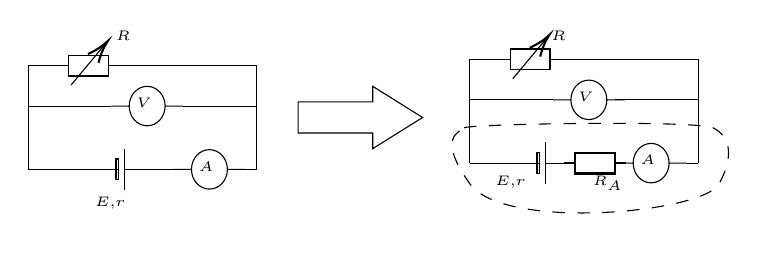
\begin{tikzpicture}[x=0.75pt,y=0.75pt,yscale=-1,xscale=1]
%uncomment if require: \path (0,300); %set diagram left start at 0, and has height of 300

%Straight Lines [id:da9223803374157449] 
\draw    (200,160) -- (230,160) ;
%Straight Lines [id:da4800046187933087] 
\draw    (310,129.5) -- (280,129.5) ;
%Shape: Battery [id:dp11572428456821915] 
\draw   (230,160) -- (243.5,160) (246.5,150) -- (246.5,170) (246.5,160) -- (260,160) (242.3,155) -- (243.5,155) -- (243.5,165) -- (242.3,165) -- (242.3,155) -- cycle ;
%Straight Lines [id:da5053925872800769] 
\draw    (200,110) -- (200,160) ;
%Straight Lines [id:da4775642533714568] 
\draw    (304.6,160) -- (310,160) ;
%Straight Lines [id:da025516599512321214] 
\draw    (310,110) -- (310,160) ;
%Shape: Output [id:dp20535874065942084] 
\draw   (278.65,160) .. controls (278.65,154.75) and (282.52,150.5) .. (287.3,150.5) .. controls (292.08,150.5) and (295.95,154.75) .. (295.95,160) .. controls (295.95,165.25) and (292.08,169.5) .. (287.3,169.5) .. controls (282.52,169.5) and (278.65,165.25) .. (278.65,160) -- cycle (270,160) -- (278.65,160) (304.6,160) -- (295.95,160) ;
%Straight Lines [id:da8691520573396538] 
\draw    (260,160) -- (270,160) ;
%Straight Lines [id:da22747916883790165] 
\draw    (200,110) -- (214,110) ;
%Shape: Resistor [id:dp2800596618552471] 
\draw   (219.4,115) -- (238.6,115) -- (238.6,105) -- (219.4,105) -- (219.4,115) -- cycle (214,110) -- (219.4,110) (238.6,110) -- (244,110) ;
%Straight Lines [id:da15708168083551777] 
\draw    (220.67,119.33) -- (237.04,99.7) ;
\draw [shift={(238.33,98.16)}, rotate = 129.83] [color={rgb, 255:red, 0; green, 0; blue, 0 }  ][line width=0.75]    (10.93,-3.29) .. controls (6.95,-1.4) and (3.31,-0.3) .. (0,0) .. controls (3.31,0.3) and (6.95,1.4) .. (10.93,3.29)   ;

%Straight Lines [id:da11312699458388331] 
\draw    (244,110) -- (310,110) ;
%Straight Lines [id:da6739961140053903] 
\draw    (274.6,129.5) -- (280,129.5) ;
%Shape: Output [id:dp7899198086186321] 
\draw   (248.65,129.5) .. controls (248.65,124.25) and (252.52,120) .. (257.3,120) .. controls (262.08,120) and (265.95,124.25) .. (265.95,129.5) .. controls (265.95,134.75) and (262.08,139) .. (257.3,139) .. controls (252.52,139) and (248.65,134.75) .. (248.65,129.5) -- cycle (240,129.5) -- (248.65,129.5) (274.6,129.5) -- (265.95,129.5) ;
%Straight Lines [id:da613270518508825] 
\draw    (230,129.5) -- (240,129.5) ;
%Straight Lines [id:da16840770867474064] 
\draw    (230,129.5) -- (200,129.5) ;
%Right Arrow [id:dp7706619739903626] 
\draw   (330,127.5) -- (366,127.5) -- (366,120) -- (390,135) -- (366,150) -- (366,142.5) -- (330,142.5) -- cycle ;
%Straight Lines [id:da4168340291806618] 
\draw    (412.81,157) -- (432.81,157) ;
%Shape: Battery [id:dp07811227108971108] 
\draw   (432.81,157) -- (446.31,157) (449.31,147) -- (449.31,167) (449.31,157) -- (462.81,157) (445.11,152) -- (446.31,152) -- (446.31,162) -- (445.11,162) -- (445.11,152) -- cycle ;
%Straight Lines [id:da5277780096339191] 
\draw    (412.81,107) -- (412.81,157) ;
%Straight Lines [id:da6252032764865012] 
\draw    (517.41,157) -- (522.81,157) ;
%Straight Lines [id:da2775418013876463] 
\draw    (522.81,107) -- (522.81,157) ;
%Shape: Output [id:dp4334794925404719] 
\draw   (491.46,157) .. controls (491.46,151.75) and (495.33,147.5) .. (500.11,147.5) .. controls (504.88,147.5) and (508.76,151.75) .. (508.76,157) .. controls (508.76,162.25) and (504.88,166.5) .. (500.11,166.5) .. controls (495.33,166.5) and (491.46,162.25) .. (491.46,157) -- cycle (482.81,157) -- (491.46,157) (517.41,157) -- (508.76,157) ;
%Straight Lines [id:da012898191912185553] 
\draw    (412.81,107) -- (426.81,107) ;
%Shape: Resistor [id:dp43127197925661176] 
\draw   (432.21,112) -- (451.41,112) -- (451.41,102) -- (432.21,102) -- (432.21,112) -- cycle (426.81,107) -- (432.21,107) (451.41,107) -- (456.81,107) ;
%Straight Lines [id:da20629449411629652] 
\draw    (433.47,116.33) -- (449.85,96.7) ;
\draw [shift={(451.13,95.16)}, rotate = 129.83] [color={rgb, 255:red, 0; green, 0; blue, 0 }  ][line width=0.75]    (10.93,-3.29) .. controls (6.95,-1.4) and (3.31,-0.3) .. (0,0) .. controls (3.31,0.3) and (6.95,1.4) .. (10.93,3.29)   ;

%Straight Lines [id:da4199064010002851] 
\draw    (456.81,107) -- (522.81,107) ;
%Straight Lines [id:da025073331712180957] 
\draw    (482.81,126.5) -- (516.81,126.5) ;
%Shape: Output [id:dp8875989383892691] 
\draw   (461.46,126.5) .. controls (461.46,121.25) and (465.33,117) .. (470.11,117) .. controls (474.88,117) and (478.76,121.25) .. (478.76,126.5) .. controls (478.76,131.75) and (474.88,136) .. (470.11,136) .. controls (465.33,136) and (461.46,131.75) .. (461.46,126.5) -- cycle (452.81,126.5) -- (461.46,126.5) (487.41,126.5) -- (478.76,126.5) ;
%Straight Lines [id:da808640618957692] 
\draw    (442.81,126.5) -- (452.81,126.5) ;
%Straight Lines [id:da3805424335033789] 
\draw    (442.81,126.5) -- (412.81,126.5) ;
%Shape: Resistor [id:dp27249147366061965] 
\draw  [color={rgb, 255:red, 0; green, 0; blue, 0 }  ,draw opacity=1 ][fill={rgb, 255:red, 255; green, 255; blue, 255 }  ,fill opacity=1 ][line width=0.75]  (463.61,152) -- (482.81,152) -- (482.81,162) -- (463.61,162) -- (463.61,152) -- cycle (458.21,157) -- (463.61,157) (482.81,157) -- (488.21,157) ;
%Straight Lines [id:da5032822234989214] 
\draw    (516.81,126.5) -- (522.81,126.5) ;
%Shape: Polygon Curved [id:ds2894822220000477] 
\draw  [dash pattern={on 4.5pt off 4.5pt}] (410,140) .. controls (412,138.09) and (522.33,136.25) .. (530,140) .. controls (537.67,143.75) and (540.61,152.91) .. (532.81,167) .. controls (525,181.09) and (429.14,189.75) .. (412.81,167) .. controls (396.47,144.25) and (408,141.91) .. (410,140) -- cycle ;

% Text Node
\draw (281,155) node [anchor=north west][inner sep=0.75pt]  [font=\tiny] [align=left] {$\displaystyle A$};
% Text Node
\draw (251,124.5) node [anchor=north west][inner sep=0.75pt]  [font=\tiny] [align=left] {$\displaystyle V$};
% Text Node
\draw (493.81,152) node [anchor=north west][inner sep=0.75pt]  [font=\tiny] [align=left] {$\displaystyle A$};
% Text Node
\draw (463.81,121.5) node [anchor=north west][inner sep=0.75pt]  [font=\tiny] [align=left] {$\displaystyle V$};
% Text Node
\draw (231,172) node [anchor=north west][inner sep=0.75pt]  [font=\tiny] [align=left] {$\displaystyle \ms E$,$\displaystyle r$};
% Text Node
\draw (241,92) node [anchor=north west][inner sep=0.75pt]  [font=\tiny] [align=left] {$\displaystyle R$};
% Text Node
\draw (450.81,92) node [anchor=north west][inner sep=0.75pt]  [font=\tiny] [align=left] {$\displaystyle R$};
% Text Node
\draw (423.81,162) node [anchor=north west][inner sep=0.75pt]  [font=\tiny] [align=left] {$\displaystyle \ms E$,$\displaystyle r$};
% Text Node
\draw (470.81,162) node [anchor=north west][inner sep=0.75pt]  [font=\tiny] [align=left] {$\displaystyle R_{A}$};
\end{tikzpicture}
\end{center}

将电源及其内阻和电流表内阻等效成新电源,则根据戴维宁定理\eqref{dwndl},新电源电动势及内阻为
$$ \ms E^{\prime} = \ms E \quad r^{\prime} = r + R_A $$

因此\textbf{电动势测量值与真实值相等,内阻测量值比真实值偏大。}

同理,对于外界法,我们将影响测量的内侧的电压表进行等效,其电路图及等效电路图如图所示

\begin{center}
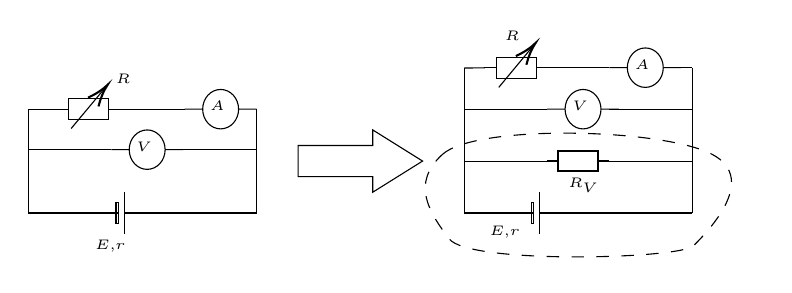
\begin{tikzpicture}[x=0.75pt,y=0.75pt,yscale=-1,xscale=1]
%uncomment if require: \path (0,300); %set diagram left start at 0, and has height of 300

%Straight Lines [id:da9223803374157449] 
\draw    (200,160) -- (230,160) ;
%Straight Lines [id:da4800046187933087] 
\draw    (310,129.5) -- (280,129.5) ;
%Shape: Battery [id:dp11572428456821915] 
\draw   (230,160) -- (243.5,160) (246.5,150) -- (246.5,170) (246.5,160) -- (260,160) (242.3,155) -- (243.5,155) -- (243.5,165) -- (242.3,165) -- (242.3,155) -- cycle ;
%Straight Lines [id:da5053925872800769] 
\draw    (200,110) -- (200,160) ;
%Straight Lines [id:da4775642533714568] 
\draw    (260,160) -- (310,160) ;
%Straight Lines [id:da025516599512321214] 
\draw    (310,110) -- (310,160) ;
%Shape: Output [id:dp20535874065942084] 
\draw   (284.05,110) .. controls (284.05,104.75) and (287.92,100.5) .. (292.7,100.5) .. controls (297.48,100.5) and (301.35,104.75) .. (301.35,110) .. controls (301.35,115.25) and (297.48,119.5) .. (292.7,119.5) .. controls (287.92,119.5) and (284.05,115.25) .. (284.05,110) -- cycle (275.4,110) -- (284.05,110) (310,110) -- (301.35,110) ;
%Straight Lines [id:da22747916883790165] 
\draw    (200,110) -- (214,110) ;
%Shape: Resistor [id:dp2800596618552471] 
\draw   (219.4,115) -- (238.6,115) -- (238.6,105) -- (219.4,105) -- (219.4,115) -- cycle (214,110) -- (219.4,110) (238.6,110) -- (244,110) ;
%Straight Lines [id:da15708168083551777] 
\draw    (220.67,119.33) -- (237.04,99.7) ;
\draw [shift={(238.33,98.16)}, rotate = 129.83] [color={rgb, 255:red, 0; green, 0; blue, 0 }  ][line width=0.75]    (10.93,-3.29) .. controls (6.95,-1.4) and (3.31,-0.3) .. (0,0) .. controls (3.31,0.3) and (6.95,1.4) .. (10.93,3.29)   ;

%Straight Lines [id:da11312699458388331] 
\draw    (244,110) -- (275.4,110) ;
%Straight Lines [id:da6739961140053903] 
\draw    (274.6,129.5) -- (280,129.5) ;
%Shape: Output [id:dp7899198086186321] 
\draw   (248.65,129.5) .. controls (248.65,124.25) and (252.52,120) .. (257.3,120) .. controls (262.08,120) and (265.95,124.25) .. (265.95,129.5) .. controls (265.95,134.75) and (262.08,139) .. (257.3,139) .. controls (252.52,139) and (248.65,134.75) .. (248.65,129.5) -- cycle (240,129.5) -- (248.65,129.5) (274.6,129.5) -- (265.95,129.5) ;
%Straight Lines [id:da613270518508825] 
\draw    (230,129.5) -- (240,129.5) ;
%Straight Lines [id:da16840770867474064] 
\draw    (230,129.5) -- (200,129.5) ;
%Right Arrow [id:dp7706619739903626] 
\draw   (330,127.5) -- (366,127.5) -- (366,120) -- (390,135) -- (366,150) -- (366,142.5) -- (330,142.5) -- cycle ;
%Straight Lines [id:da4168340291806618] 
\draw    (410,160) -- (430,160) ;
%Shape: Battery [id:dp07811227108971108] 
\draw   (430,160) -- (443.5,160) (446.5,150) -- (446.5,170) (446.5,160) -- (460,160) (442.3,155) -- (443.5,155) -- (443.5,165) -- (442.3,165) -- (442.3,155) -- cycle ;
%Straight Lines [id:da5277780096339191] 
\draw    (410,90) -- (410,160) ;
%Straight Lines [id:da6252032764865012] 
\draw    (460,160) -- (520,160) ;
%Straight Lines [id:da2775418013876463] 
\draw    (520,90) -- (520,160) ;
%Shape: Output [id:dp4334794925404719] 
\draw   (488.65,90) .. controls (488.65,84.75) and (492.52,80.5) .. (497.3,80.5) .. controls (502.08,80.5) and (505.95,84.75) .. (505.95,90) .. controls (505.95,95.25) and (502.08,99.5) .. (497.3,99.5) .. controls (492.52,99.5) and (488.65,95.25) .. (488.65,90) -- cycle (480,90) -- (488.65,90) (514.6,90) -- (505.95,90) ;
%Straight Lines [id:da012898191912185553] 
\draw    (410,90.19) -- (420,90.06) ;
%Shape: Resistor [id:dp43127197925661176] 
\draw   (425.43,95.12) -- (444.74,95.12) -- (444.74,85) -- (425.43,85) -- (425.43,95.12) -- cycle (420,90.06) -- (425.43,90.06) (444.74,90.06) -- (450.17,90.06) ;
%Straight Lines [id:da20629449411629652] 
\draw    (426.7,99.5) -- (443.19,79.63) ;
\draw [shift={(444.46,78.09)}, rotate = 129.67] [color={rgb, 255:red, 0; green, 0; blue, 0 }  ][line width=0.75]    (10.93,-3.29) .. controls (6.95,-1.4) and (3.31,-0.3) .. (0,0) .. controls (3.31,0.3) and (6.95,1.4) .. (10.93,3.29)   ;

%Straight Lines [id:da4199064010002851] 
\draw    (450,90) -- (480,90) ;
%Straight Lines [id:da025073331712180957] 
\draw    (480,110) -- (520,110) ;
%Shape: Output [id:dp8875989383892691] 
\draw   (458.65,110) .. controls (458.65,104.75) and (462.52,100.5) .. (467.3,100.5) .. controls (472.08,100.5) and (475.95,104.75) .. (475.95,110) .. controls (475.95,115.25) and (472.08,119.5) .. (467.3,119.5) .. controls (462.52,119.5) and (458.65,115.25) .. (458.65,110) -- cycle (450,110) -- (458.65,110) (484.6,110) -- (475.95,110) ;
%Straight Lines [id:da808640618957692] 
\draw    (440,110) -- (450,110) ;
%Straight Lines [id:da3805424335033789] 
\draw    (440,110) -- (410,110) ;
%Shape: Resistor [id:dp27249147366061965] 
\draw  [color={rgb, 255:red, 0; green, 0; blue, 0 }  ,draw opacity=1 ][fill={rgb, 255:red, 255; green, 255; blue, 255 }  ,fill opacity=1 ][line width=0.75]  (455.4,130) -- (474.6,130) -- (474.6,140) -- (455.4,140) -- (455.4,130) -- cycle (450,135) -- (455.4,135) (474.6,135) -- (480,135) ;
%Straight Lines [id:da5032822234989214] 
\draw    (480,135) -- (520,135) ;
%Shape: Polygon Curved [id:ds2894822220000477] 
\draw  [dash pattern={on 4.5pt off 4.5pt}] (399.5,131.84) .. controls (415.01,117.67) and (499.33,119) .. (526.84,130.5) .. controls (554.34,142.01) and (526.84,169.5) .. (520.5,175.84) .. controls (514.17,182.17) and (412.17,184.84) .. (402.84,172.5) .. controls (393.5,160.17) and (384,146) .. (399.5,131.84) -- cycle ;
%Straight Lines [id:da8501291218143447] 
\draw    (410,135) -- (450,135) ;
%Straight Lines [id:da21442590370161208] 
\draw    (514.6,90) -- (520,90) ;

% Text Node
\draw (286.4,105) node [anchor=north west][inner sep=0.75pt]  [font=\tiny] [align=left] {$\displaystyle A$};
% Text Node
\draw (251,124.5) node [anchor=north west][inner sep=0.75pt]  [font=\tiny] [align=left] {$\displaystyle V$};
% Text Node
\draw (491,85.17) node [anchor=north west][inner sep=0.75pt]  [font=\tiny] [align=left] {$\displaystyle A$};
% Text Node
\draw (461,105) node [anchor=north west][inner sep=0.75pt]  [font=\tiny] [align=left] {$\displaystyle V$};
% Text Node
\draw (231,172) node [anchor=north west][inner sep=0.75pt]  [font=\tiny] [align=left] {$\displaystyle \ms E$,$\displaystyle r$};
% Text Node
\draw (241,92) node [anchor=north west][inner sep=0.75pt]  [font=\tiny] [align=left] {$\displaystyle R$};
% Text Node
\draw (428.33,71) node [anchor=north west][inner sep=0.75pt]  [font=\tiny] [align=left] {$\displaystyle R$};
% Text Node
\draw (421,165) node [anchor=north west][inner sep=0.75pt]  [font=\tiny] [align=left] {$\displaystyle \ms E$,$\displaystyle r$};
% Text Node
\draw (459,142) node [anchor=north west][inner sep=0.75pt]  [font=\tiny] [align=left] {$\displaystyle R_{V}$};
\end{tikzpicture}

\end{center}

将电源及其内阻和电压表内阻等效成新电源,则根据戴维宁定理\eqref{dwndl},新电源电动势及内阻为
$$ \ms E^{\prime} = \frac{ \ms E R_V}{R_V + r} \quad r^{\prime} = \frac{r R_V}{r + R_V} $$

因此\textbf{电动势测量值比真实值偏小,内阻测量值比真实值偏小。}
\end{ep}

对于选择题,若遇到$\frac{\Delta U}{\Delta I}$且其对应的电阻正在变化,则一般情况下可以使用等效源进行等效,其$\frac{\Delta U}{\Delta I}$等于新内阻。具体可见如下例题。

\begin{ep}{练习题}{}

\begin{center}
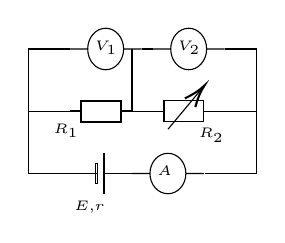
\begin{tikzpicture}[x=0.75pt,y=0.75pt,yscale=-1,xscale=1]
%uncomment if require: \path (0,300); %set diagram left start at 0, and has height of 300

%Straight Lines [id:da14551039289024326] 
\draw    (130,220) -- (150,220) ;
%Straight Lines [id:da3295959610713812] 
\draw    (150,160) -- (130,160) ;
%Shape: Battery [id:dp8317998227732923] 
\draw   (150,220) -- (163.5,220) (166.5,210) -- (166.5,230) (166.5,220) -- (180,220) (162.3,215) -- (163.5,215) -- (163.5,225) -- (162.3,225) -- (162.3,215) -- cycle ;
%Straight Lines [id:da6993800641983081] 
\draw    (130,160) -- (130,220) ;
%Straight Lines [id:da47030402702453067] 
\draw    (215,220) -- (240,220) ;
%Straight Lines [id:da10115275650248856] 
\draw    (240,160) -- (240,220) ;
%Shape: Output [id:dp34471276111404703] 
\draw   (188.65,220) .. controls (188.65,214.62) and (192.52,210.26) .. (197.3,210.26) .. controls (202.08,210.26) and (205.95,214.62) .. (205.95,220) .. controls (205.95,225.38) and (202.08,229.74) .. (197.3,229.74) .. controls (192.52,229.74) and (188.65,225.38) .. (188.65,220) -- cycle (180,220) -- (188.65,220) (214.6,220) -- (205.95,220) ;
%Straight Lines [id:da2535463577123036] 
\draw    (220,190) -- (240,190) ;
%Shape: Resistor [id:dp2889455083490655] 
\draw   (195.4,195) -- (214.6,195) -- (214.6,185) -- (195.4,185) -- (195.4,195) -- cycle (190,190) -- (195.4,190) (214.6,190) -- (220,190) ;
%Straight Lines [id:da6959465546040076] 
\draw    (197.33,198.67) -- (213.71,179.03) ;
\draw [shift={(214.99,177.5)}, rotate = 129.83] [color={rgb, 255:red, 0; green, 0; blue, 0 }  ][line width=0.75]    (10.93,-3.29) .. controls (6.95,-1.4) and (3.31,-0.3) .. (0,0) .. controls (3.31,0.3) and (6.95,1.4) .. (10.93,3.29)   ;
%Straight Lines [id:da7548896744967672] 
\draw    (224.6,160) -- (240,160) ;
%Straight Lines [id:da05255225869571456] 
\draw    (184.6,160) -- (190,160) ;
%Shape: Output [id:dp7402485705608346] 
\draw   (158.65,160) .. controls (158.65,154.48) and (162.52,150) .. (167.3,150) .. controls (172.08,150) and (175.95,154.48) .. (175.95,160) .. controls (175.95,165.52) and (172.08,170) .. (167.3,170) .. controls (162.52,170) and (158.65,165.52) .. (158.65,160) -- cycle (150,160) -- (158.65,160) (184.6,160) -- (175.95,160) ;
%Straight Lines [id:da7775464807313777] 
\draw    (180,190) -- (190,190) ;
%Straight Lines [id:da5256323795807551] 
\draw    (150,190) -- (130,190) ;
%Shape: Resistor [id:dp7893409265728679] 
\draw  [color={rgb, 255:red, 0; green, 0; blue, 0 }  ,draw opacity=1 ][fill={rgb, 255:red, 255; green, 255; blue, 255 }  ,fill opacity=1 ][line width=0.75]  (155.4,185) -- (174.6,185) -- (174.6,195) -- (155.4,195) -- (155.4,185) -- cycle (150,190) -- (155.4,190) (174.6,190) -- (180,190) ;
%Shape: Output [id:dp686244368823177] 
\draw   (198.65,160) .. controls (198.65,154.48) and (202.52,150) .. (207.3,150) .. controls (212.08,150) and (215.95,154.48) .. (215.95,160) .. controls (215.95,165.52) and (212.08,170) .. (207.3,170) .. controls (202.52,170) and (198.65,165.52) .. (198.65,160) -- cycle (190,160) -- (198.65,160) (224.6,160) -- (215.95,160) ;
%Straight Lines [id:da6913018383920955] 
\draw    (180,160) -- (180,190) ;

% Text Node
\draw (191,215) node [anchor=north west][inner sep=0.75pt]  [font=\tiny] [align=left] {$\displaystyle A$};
% Text Node
\draw (161,155) node [anchor=north west][inner sep=0.75pt]  [font=\tiny] [align=left] {$\displaystyle V_{1}$};
% Text Node
\draw (151,232) node [anchor=north west][inner sep=0.75pt]  [font=\tiny] [align=left] {$\displaystyle E$,$\displaystyle r$};
% Text Node
\draw (141,195) node [anchor=north west][inner sep=0.75pt]  [font=\tiny] [align=left] {$\displaystyle R_{1}$};
% Text Node
\draw (201,155) node [anchor=north west][inner sep=0.75pt]  [font=\tiny] [align=left] {$\displaystyle V_{2}$};
% Text Node
\draw (211,197) node [anchor=north west][inner sep=0.75pt]  [font=\tiny] [align=left] {$\displaystyle R_{2}$};
\end{tikzpicture}
\end{center}

如图所示的电路中,各电表为理想电表,电源内阻不能忽略,当可变电阻$R_2$减小了$\Delta R$过程中,设$V_1$、$V_2$、$A$的读数分别是$U_1$、$U_2$、$I$;$V_1$、$V_2$、$A$的读数的变化量分别为$\Delta U_1$、$\Delta U_2$、$\Delta I$,则下列说法正确的是()

\begin{enumerate}[label=(\Alph*)]
  \item $U_2$与$I$的比值减小,$U_2$与$I$的乘积也一定减小
  \item $U_1$与$I$的比值不变,$U_1$与$I$的乘积也一定不变
  \item $\Delta U_2$与$\Delta I$的比值等于$\Delta U_1$与$\Delta I$的比值
  \item $\Delta U_1$与$\Delta I$的比值等于任何时刻$U_1$与$I$的比值
\end{enumerate}

~\\
$R_2$变小,根据“串反并同”(见下一章\eqref{s_cfbt})知,$U_1$增大,$U_2$减小,$I$增大,故$U_1$与$I$乘积不为定值。选项B错误。

将除了$R_2$外其他部分等效成新电源,则新电源$\ms E^{\prime} = \ms E = E$、$r^{\prime} = r + R_1$。由外电路最大功率知,$R_2$越接近$r + R_1$,其功率越大。但体中并未知道初始时$R_2$阻值与$r + R_1$关系,故无从判断$U_2 I$的变化趋势,故选项A错误。

根据上面电路等效知,$U_2$相当于测等效后电源路端电压,$I$相当于测电路电流,故$\frac{\Delta U_2}{\Delta I} = r + R_1$,而$\frac{\Delta U_1}{\Delta I} = R_1$,故选项C错误。

$\frac{U_1}{I} = \frac{\Delta U_1}{\Delta I} = R_1$,$R_1$为定值,故选项D正确。综上所述,答案为$D$。
\end{ep}

\section{串反并同及广义串并联判断}
\label{s_cfbt}

在电路分析中有这样一条实用的定理

\begin{theo}{串反并同}{}
\textbf{在电源内阻不可忽略的情况下,若只有单个电阻变化},则与该电阻广义串联的电阻或电表(电表本质上也是内阻,不过可以显示电学值而已),其电压、电流、功率的变化与电阻的变化相反,即\textbf{“串反”};与该电阻广义并联的电阻或电表,其电压、电流、功率的变化与电阻的变化相同,即\textbf{“并同”}
\end{theo}

这里需要对所谓的“广义串联”以及“广义并联” 进行定义和解释说明。

\begin{defi}[label=gycbl]{“广义串联”和“广义并联”}{}
电路中若经过电阻A的电流在一个完整回路内\textbf{可以流过}电阻B,则这两电阻为\textbf{等效串联}。

电路中若经过电阻A的电流在一个完整回路内\textbf{不可能流过}电阻B,则这两电阻为\textbf{等效并联}。
\end{defi}

上面的定理可能有些抽象,下面有一种可操作的方法,\textbf{并不完全严谨,但在高中阶段绝大部分可用}。

\begin{center}
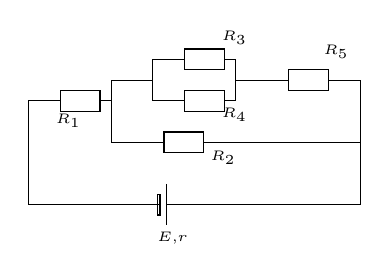
\begin{tikzpicture}[x=0.75pt,y=0.75pt,yscale=-1,xscale=1]
%uncomment if require: \path (0,300); %set diagram left start at 0, and has height of 300

%Shape: Battery [id:dp41038864580231404] 
\draw   (160,130) -- (173.5,130) (176.5,120) -- (176.5,140) (176.5,130) -- (190,130) (172.3,125) -- (173.5,125) -- (173.5,135) -- (172.3,135) -- (172.3,125) -- cycle ;
%Straight Lines [id:da3163365738659809] 
\draw    (190,130) -- (270,130) ;
%Straight Lines [id:da05173675712222314] 
\draw    (110,80) -- (110,130) ;
%Straight Lines [id:da47804297862757794] 
\draw    (110,80) -- (120,80) ;
%Straight Lines [id:da9057643206618209] 
\draw    (150,70) -- (150,100) ;
%Shape: Resistor [id:dp9965546099949054] 
\draw   (125.4,75) -- (144.6,75) -- (144.6,85) -- (125.4,85) -- (125.4,75) -- cycle (120,80) -- (125.4,80) (144.6,80) -- (150,80) ;
%Straight Lines [id:da0755765621865847] 
\draw    (170,60) -- (170,80) ;
%Straight Lines [id:da5506543591062112] 
\draw    (110,130) -- (160,130) ;
%Shape: Resistor [id:dp5943525570087891] 
\draw   (175.4,95) -- (194.6,95) -- (194.6,105) -- (175.4,105) -- (175.4,95) -- cycle (170,100) -- (175.4,100) (194.6,100) -- (200,100) ;
%Straight Lines [id:da20458298027628818] 
\draw    (150,100) -- (170,100) ;
%Straight Lines [id:da4442305975937406] 
\draw    (200,100) -- (270,100) ;
%Straight Lines [id:da35717809113951704] 
\draw    (150,70) -- (170,70) ;
%Straight Lines [id:da3625645367127812] 
\draw    (170,80) -- (180,80) ;
%Shape: Resistor [id:dp27044674641893796] 
\draw   (185.4,75) -- (204.6,75) -- (204.6,85) -- (185.4,85) -- (185.4,75) -- cycle (180,80) -- (185.4,80) (204.6,80) -- (210,80) ;
%Shape: Resistor [id:dp9888935439946336] 
\draw   (185.4,55) -- (204.6,55) -- (204.6,65) -- (185.4,65) -- (185.4,55) -- cycle (180,60) -- (185.4,60) (204.6,60) -- (210,60) ;
%Straight Lines [id:da2570097891204668] 
\draw    (170,60) -- (180,60) ;
%Straight Lines [id:da8597169745318671] 
\draw    (210,60) -- (210,80) ;
%Straight Lines [id:da6968281670670353] 
\draw    (210,70) -- (230,70) ;
%Shape: Resistor [id:dp9106011423679721] 
\draw   (235.4,65) -- (254.6,65) -- (254.6,75) -- (235.4,75) -- (235.4,65) -- cycle (230,70) -- (235.4,70) (254.6,70) -- (260,70) ;
%Straight Lines [id:da7437742845966437] 
\draw    (260,70) -- (270,70) ;
%Straight Lines [id:da46641133055265294] 
\draw    (270,70) -- (270,130) ;

% Text Node
\draw (171,142) node [anchor=north west][inner sep=0.75pt]  [font=\tiny] [align=left] {$\displaystyle \ms E$,$\displaystyle r$};
% Text Node
\draw (122,85) node [anchor=north west][inner sep=0.75pt]  [font=\tiny] [align=left] {$\displaystyle R_{1}$};
% Text Node
\draw (196.6,103) node [anchor=north west][inner sep=0.75pt]  [font=\tiny] [align=left] {$\displaystyle R_{2}$};
% Text Node
\draw (202,45) node [anchor=north west][inner sep=0.75pt]  [font=\tiny] [align=left] {$\displaystyle R_{3}$};
% Text Node
\draw (202,82) node [anchor=north west][inner sep=0.75pt]  [font=\tiny] [align=left] {$\displaystyle R_{4}$};
% Text Node
\draw (251,52) node [anchor=north west][inner sep=0.75pt]  [font=\tiny] [align=left] {$\displaystyle R_{5}$};


\end{tikzpicture}

\end{center}

如图所示,现有一如上较复杂的电路,对于$R_1$和$R_5$,我们\textbf{可以用一个经过电源的回路将这两个电阻相连,若连接此两电阻可以经过电源,我们认为其为等效串联},如下左图所示。

\begin{minipage}[b]{0.45\linewidth}
\begin{center}

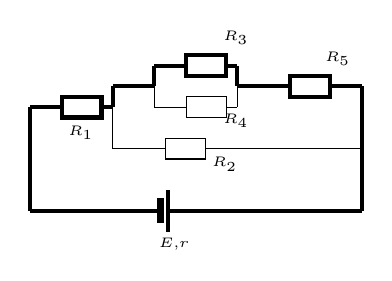
\begin{tikzpicture}[x=0.75pt,y=0.75pt,yscale=-1,xscale=1]
%uncomment if require: \path (0,300); %set diagram left start at 0, and has height of 300

%Shape: Battery [id:dp41038864580231404] 
\draw  [color={rgb, 255:red, 0; green, 0; blue, 0 }  ,draw opacity=1 ][line width=1.5]  (160,130) -- (173.5,130) (176.5,120) -- (176.5,140) (176.5,130) -- (190,130) (172.3,125) -- (173.5,125) -- (173.5,135) -- (172.3,135) -- (172.3,125) -- cycle ;
%Straight Lines [id:da3163365738659809] 
\draw [color={rgb, 255:red, 0; green, 0; blue, 0 }  ,draw opacity=1 ][line width=1.5]    (190,130) -- (270,130) ;
%Straight Lines [id:da05173675712222314] 
\draw [color={rgb, 255:red, 0; green, 0; blue, 0 }  ,draw opacity=1 ][line width=1.5]    (110,80) -- (110,130) ;
%Straight Lines [id:da47804297862757794] 
\draw [color={rgb, 255:red, 0; green, 0; blue, 0 }  ,draw opacity=1 ][line width=1.5]    (110,80) -- (120,80) ;
%Straight Lines [id:da9057643206618209] 
\draw [color={rgb, 255:red, 0; green, 0; blue, 0 }  ,draw opacity=1 ][line width=1.5]    (150,70) -- (150,80) ;
%Shape: Resistor [id:dp9965546099949054] 
\draw  [color={rgb, 255:red, 0; green, 0; blue, 0 }  ,draw opacity=1 ][line width=1.5]  (125.4,75) -- (144.6,75) -- (144.6,85) -- (125.4,85) -- (125.4,75) -- cycle (120,80) -- (125.4,80) (144.6,80) -- (150,80) ;
%Straight Lines [id:da0755765621865847] 
\draw [color={rgb, 255:red, 0; green, 0; blue, 0 }  ,draw opacity=1 ][line width=1.5]    (170,60) -- (170,70) ;
%Straight Lines [id:da5506543591062112] 
\draw [color={rgb, 255:red, 0; green, 0; blue, 0 }  ,draw opacity=1 ][line width=1.5]    (110,130) -- (160,130) ;
%Shape: Resistor [id:dp5943525570087891] 
\draw  [color={rgb, 255:red, 0; green, 0; blue, 0 }  ,draw opacity=1 ] (175.4,95) -- (194.6,95) -- (194.6,105) -- (175.4,105) -- (175.4,95) -- cycle (170,100) -- (175.4,100) (194.6,100) -- (200,100) ;
%Straight Lines [id:da20458298027628818] 
\draw [color={rgb, 255:red, 0; green, 0; blue, 0 }  ,draw opacity=1 ]   (150,100) -- (170,100) ;
%Straight Lines [id:da4442305975937406] 
\draw [color={rgb, 255:red, 0; green, 0; blue, 0 }  ,draw opacity=1 ]   (200,100) -- (270,100) ;
%Straight Lines [id:da35717809113951704] 
\draw [color={rgb, 255:red, 0; green, 0; blue, 0 }  ,draw opacity=1 ][line width=1.5]    (150,70) -- (170,70) ;
%Straight Lines [id:da3625645367127812] 
\draw [color={rgb, 255:red, 0; green, 0; blue, 0 }  ,draw opacity=1 ]   (170,80) -- (180,80) ;
%Shape: Resistor [id:dp27044674641893796] 
\draw  [color={rgb, 255:red, 0; green, 0; blue, 0 }  ,draw opacity=1 ] (185.4,75) -- (204.6,75) -- (204.6,85) -- (185.4,85) -- (185.4,75) -- cycle (180,80) -- (185.4,80) (204.6,80) -- (210,80) ;
%Shape: Resistor [id:dp9888935439946336] 
\draw  [color={rgb, 255:red, 0; green, 0; blue, 0 }  ,draw opacity=1 ][line width=1.5]  (185.4,55) -- (204.6,55) -- (204.6,65) -- (185.4,65) -- (185.4,55) -- cycle (180,60) -- (185.4,60) (204.6,60) -- (210,60) ;
%Straight Lines [id:da2570097891204668] 
\draw [color={rgb, 255:red, 0; green, 0; blue, 0 }  ,draw opacity=1 ][line width=1.5]    (170,60) -- (180,60) ;
%Straight Lines [id:da8597169745318671] 
\draw [color={rgb, 255:red, 0; green, 0; blue, 0 }  ,draw opacity=1 ][line width=1.5]    (210,60) -- (210,70) ;
%Straight Lines [id:da6968281670670353] 
\draw [color={rgb, 255:red, 0; green, 0; blue, 0 }  ,draw opacity=1 ][line width=1.5]    (210,70) -- (230,70) ;
%Shape: Resistor [id:dp9106011423679721] 
\draw  [color={rgb, 255:red, 0; green, 0; blue, 0 }  ,draw opacity=1 ][fill={rgb, 255:red, 255; green, 255; blue, 255 }  ,fill opacity=1 ][line width=1.5]  (235.4,65) -- (254.6,65) -- (254.6,75) -- (235.4,75) -- (235.4,65) -- cycle (230,70) -- (235.4,70) (254.6,70) -- (260,70) ;
%Straight Lines [id:da7437742845966437] 
\draw [color={rgb, 255:red, 0; green, 0; blue, 0 }  ,draw opacity=1 ][line width=1.5]    (260,70) -- (270,70) ;
%Straight Lines [id:da46641133055265294] 
\draw [color={rgb, 255:red, 0; green, 0; blue, 0 }  ,draw opacity=1 ][line width=1.5]    (270,70) -- (270,100) -- (270,130) ;
%Straight Lines [id:da7904655950974608] 
\draw [color={rgb, 255:red, 0; green, 0; blue, 0 }  ,draw opacity=1 ]   (210,70) -- (210,80) ;
%Straight Lines [id:da09045289558828129] 
\draw [color={rgb, 255:red, 0; green, 0; blue, 0 }  ,draw opacity=1 ]   (170,70) -- (170,80) ;
%Straight Lines [id:da8466930385719886] 
\draw [color={rgb, 255:red, 0; green, 0; blue, 0 }  ,draw opacity=1 ]   (150,80) -- (150,100) ;

% Text Node
\draw (171,142) node [anchor=north west][inner sep=0.75pt]  [font=\tiny] [align=left] {$\displaystyle \ms E$,$\displaystyle r$};
% Text Node
\draw (127.4,88) node [anchor=north west][inner sep=0.75pt]  [font=\tiny] [align=left] {$\displaystyle R_{1}$};
% Text Node
\draw (196.6,103) node [anchor=north west][inner sep=0.75pt]  [font=\tiny] [align=left] {$\displaystyle R_{2}$};
% Text Node
\draw (202,42) node [anchor=north west][inner sep=0.75pt]  [font=\tiny] [align=left] {$\displaystyle R_{3}$};
% Text Node
\draw (202,82) node [anchor=north west][inner sep=0.75pt]  [font=\tiny] [align=left] {$\displaystyle R_{4}$};
% Text Node
\draw (251,52) node [anchor=north west][inner sep=0.75pt]  [font=\tiny] [align=left] {$\displaystyle R_{5}$};
\end{tikzpicture}
\end{center}
\end{minipage}
\hfill
\begin{minipage}[b]{0.45\linewidth}
\begin{center}
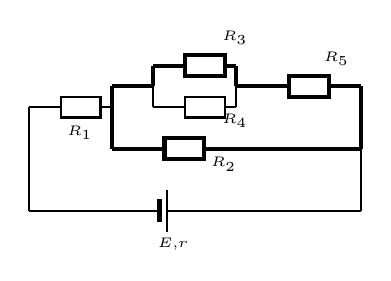
\begin{tikzpicture}[x=0.75pt,y=0.75pt,yscale=-1,xscale=1]
%uncomment if require: \path (0,300); %set diagram left start at 0, and has height of 300

%Shape: Battery [id:dp41038864580231404] 
\draw  [color={rgb, 255:red, 0; green, 0; blue, 0 }  ,draw opacity=1 ][line width=0.75]  (160,130) -- (173.5,130) (176.5,120) -- (176.5,140) (176.5,130) -- (190,130) (172.3,125) -- (173.5,125) -- (173.5,135) -- (172.3,135) -- (172.3,125) -- cycle ;
%Straight Lines [id:da3163365738659809] 
\draw [color={rgb, 255:red, 0; green, 0; blue, 0 }  ,draw opacity=1 ][line width=0.75]    (190,130) -- (270,130) ;
%Straight Lines [id:da05173675712222314] 
\draw [color={rgb, 255:red, 0; green, 0; blue, 0 }  ,draw opacity=1 ][line width=0.75]    (110,80) -- (110,130) ;
%Straight Lines [id:da47804297862757794] 
\draw [color={rgb, 255:red, 0; green, 0; blue, 0 }  ,draw opacity=1 ][line width=0.75]    (110,80) -- (120,80) ;
%Straight Lines [id:da9057643206618209] 
\draw [color={rgb, 255:red, 0; green, 0; blue, 0 }  ,draw opacity=1 ][line width=1.5]    (150,70) -- (150,80) ;
%Shape: Resistor [id:dp9965546099949054] 
\draw  [color={rgb, 255:red, 0; green, 0; blue, 0 }  ,draw opacity=1 ][line width=0.75]  (125.4,75) -- (144.6,75) -- (144.6,85) -- (125.4,85) -- (125.4,75) -- cycle (120,80) -- (125.4,80) (144.6,80) -- (150,80) ;
%Straight Lines [id:da0755765621865847] 
\draw [color={rgb, 255:red, 0; green, 0; blue, 0 }  ,draw opacity=1 ][line width=1.5]    (170,60) -- (170,70) ;
%Straight Lines [id:da5506543591062112] 
\draw [color={rgb, 255:red, 0; green, 0; blue, 0 }  ,draw opacity=1 ][line width=0.75]    (110,130) -- (160,130) ;
%Shape: Resistor [id:dp5943525570087891] 
\draw  [color={rgb, 255:red, 0; green, 0; blue, 0 }  ,draw opacity=1 ][line width=1.5]  (175.4,95) -- (194.6,95) -- (194.6,105) -- (175.4,105) -- (175.4,95) -- cycle (170,100) -- (175.4,100) (194.6,100) -- (200,100) ;
%Straight Lines [id:da20458298027628818] 
\draw [color={rgb, 255:red, 0; green, 0; blue, 0 }  ,draw opacity=1 ][line width=1.5]    (150,100) -- (170,100) ;
%Straight Lines [id:da4442305975937406] 
\draw [color={rgb, 255:red, 0; green, 0; blue, 0 }  ,draw opacity=1 ][line width=1.5]    (200,100) -- (270,100) ;
%Straight Lines [id:da35717809113951704] 
\draw [color={rgb, 255:red, 0; green, 0; blue, 0 }  ,draw opacity=1 ][line width=1.5]    (150,70) -- (170,70) ;
%Straight Lines [id:da3625645367127812] 
\draw [color={rgb, 255:red, 0; green, 0; blue, 0 }  ,draw opacity=1 ][line width=0.75]    (170,80) -- (180,80) ;
%Shape: Resistor [id:dp27044674641893796] 
\draw  [color={rgb, 255:red, 0; green, 0; blue, 0 }  ,draw opacity=1 ][line width=0.75]  (185.4,75) -- (204.6,75) -- (204.6,85) -- (185.4,85) -- (185.4,75) -- cycle (180,80) -- (185.4,80) (204.6,80) -- (210,80) ;
%Shape: Resistor [id:dp9888935439946336] 
\draw  [color={rgb, 255:red, 0; green, 0; blue, 0 }  ,draw opacity=1 ][line width=1.5]  (185.4,55) -- (204.6,55) -- (204.6,65) -- (185.4,65) -- (185.4,55) -- cycle (180,60) -- (185.4,60) (204.6,60) -- (210,60) ;
%Straight Lines [id:da2570097891204668] 
\draw [color={rgb, 255:red, 0; green, 0; blue, 0 }  ,draw opacity=1 ][line width=1.5]    (170,60) -- (180,60) ;
%Straight Lines [id:da8597169745318671] 
\draw [color={rgb, 255:red, 0; green, 0; blue, 0 }  ,draw opacity=1 ][line width=1.5]    (210,60) -- (210,70) ;
%Straight Lines [id:da6968281670670353] 
\draw [color={rgb, 255:red, 0; green, 0; blue, 0 }  ,draw opacity=1 ][line width=1.5]    (210,70) -- (230,70) ;
%Shape: Resistor [id:dp9106011423679721] 
\draw  [color={rgb, 255:red, 0; green, 0; blue, 0 }  ,draw opacity=1 ][fill={rgb, 255:red, 255; green, 255; blue, 255 }  ,fill opacity=1 ][line width=1.5]  (235.4,65) -- (254.6,65) -- (254.6,75) -- (235.4,75) -- (235.4,65) -- cycle (230,70) -- (235.4,70) (254.6,70) -- (260,70) ;
%Straight Lines [id:da7437742845966437] 
\draw [color={rgb, 255:red, 0; green, 0; blue, 0 }  ,draw opacity=1 ][line width=1.5]    (260,70) -- (270,70) ;
%Straight Lines [id:da46641133055265294] 
\draw [color={rgb, 255:red, 0; green, 0; blue, 0 }  ,draw opacity=1 ][line width=1.5]    (270,70) -- (270,100) ;
%Straight Lines [id:da7904655950974608] 
\draw [color={rgb, 255:red, 0; green, 0; blue, 0 }  ,draw opacity=1 ][line width=0.75]    (210,70) -- (210,80) ;
%Straight Lines [id:da09045289558828129] 
\draw [color={rgb, 255:red, 0; green, 0; blue, 0 }  ,draw opacity=1 ][line width=0.75]    (170,70) -- (170,80) ;
%Straight Lines [id:da8466930385719886] 
\draw [color={rgb, 255:red, 0; green, 0; blue, 0 }  ,draw opacity=1 ][line width=1.5]    (150,80) -- (150,100) ;
%Straight Lines [id:da9186238470693386] 
\draw [color={rgb, 255:red, 0; green, 0; blue, 0 }  ,draw opacity=1 ][line width=0.75]    (270,100) -- (270,130) ;

% Text Node
\draw (171,142) node [anchor=north west][inner sep=0.75pt]  [font=\tiny] [align=left] {$\displaystyle \ms E$,$\displaystyle r$};
% Text Node
\draw (127.4,88) node [anchor=north west][inner sep=0.75pt]  [font=\tiny] [align=left] {$\displaystyle R_{1}$};
% Text Node
\draw (196.6,103) node [anchor=north west][inner sep=0.75pt]  [font=\tiny] [align=left] {$\displaystyle R_{2}$};
% Text Node
\draw (202,42) node [anchor=north west][inner sep=0.75pt]  [font=\tiny] [align=left] {$\displaystyle R_{3}$};
% Text Node
\draw (202,82) node [anchor=north west][inner sep=0.75pt]  [font=\tiny] [align=left] {$\displaystyle R_{4}$};
% Text Node
\draw (251,52) node [anchor=north west][inner sep=0.75pt]  [font=\tiny] [align=left] {$\displaystyle R_{5}$};

\end{tikzpicture}
\end{center}
\end{minipage}

对于$R_2$和$R_5$,我们\textbf{不可能用一个经过电源的回路将这两个电阻相连,若连接此两电阻不可以经过电源,我们认为其为等效并联},如上右图所示。\footnote{这里对于如电桥类问题并不适用,因为随着电桥某一桥臂电阻的改变,其经过中间的电阻的电流方向会发生改变,从而改变其等效串并联关系。在此情况下只能根据前文“广义串并联”的定义\eqref{gycbl}分情况进行判断。}

这里需要注意,串反并同存在使用条件,如下

\begin{mk}{易错提醒}{}
当且仅当\textbf{电源存在内阻}以及\textbf{只有单个电阻变化}时,才可以运用“串反并同”。
\end{mk}

当然,根据前文戴维宁定理\eqref{dwndl},可以通过将不存在内阻的理想电压源跟外电路的电阻等效成具有内阻的电源而使用串反并同,具体可见如下例题。

\begin{ep}{2009·广东}{}

\begin{center}

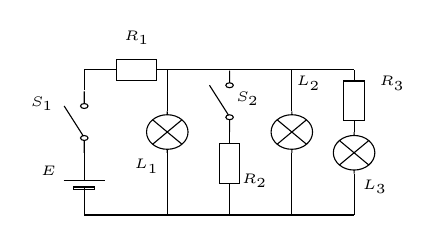
\begin{tikzpicture}[x=0.75pt,y=0.75pt,yscale=-1,xscale=1]
%uncomment if require: \path (0,300); %set diagram left start at 0, and has height of 300

%Shape: Battery [id:dp797984114545808] 
\draw   (100,170) -- (100,156.5) (90,153.5) -- (110,153.5) (100,153.5) -- (100,140) (95,157.7) -- (95,156.5) -- (105,156.5) -- (105,157.7) -- (95,157.7) -- cycle ;
%Shape: Simple Switch [id:dp4334800063265021] 
\draw   (100,140) -- (100,134.07) (100,116.29) -- (100,110.37) (99.39,131.7) -- (90.32,117.48) (100,118.66) .. controls (99,118.66) and (98.18,118.13) .. (98.18,117.48) .. controls (98.18,116.82) and (99,116.29) .. (100,116.29) .. controls (101,116.29) and (101.82,116.82) .. (101.82,117.48) .. controls (101.82,118.13) and (101,118.66) .. (100,118.66) -- cycle (100,134.07) .. controls (99,134.07) and (98.18,133.54) .. (98.18,132.89) .. controls (98.18,132.23) and (99,131.7) .. (100,131.7) .. controls (101,131.7) and (101.82,132.23) .. (101.82,132.89) .. controls (101.82,133.54) and (101,134.07) .. (100,134.07) -- cycle ;
%Shape: Resistor [id:dp901312688402967] 
\draw   (115.4,95) -- (134.6,95) -- (134.6,105) -- (115.4,105) -- (115.4,95) -- cycle (110,100) -- (115.4,100) (134.6,100) -- (140,100) ;
%Straight Lines [id:da2657385353492341] 
\draw    (100,110) -- (100,100) ;
%Straight Lines [id:da5416440059996896] 
\draw    (100,100) -- (110,100) ;
%Shape: Light Bulb [id:dp598022898779403] 
\draw   (140,138.33) .. controls (134.48,138.33) and (130,134.6) .. (130,130) .. controls (130,125.4) and (134.48,121.67) .. (140,121.67) .. controls (145.52,121.67) and (150,125.4) .. (150,130) .. controls (150,134.6) and (145.52,138.33) .. (140,138.33) -- cycle (132.88,135.93) -- (147.12,124.07) (132.88,124.07) -- (147.12,135.93) (140,140) -- (140,138.33) (140,121.67) -- (140,120) ;
%Straight Lines [id:da4277642056179305] 
\draw    (140,100) -- (140,120) ;
%Straight Lines [id:da9223803374157449] 
\draw    (100,170) -- (230,170) ;
%Straight Lines [id:da4800046187933087] 
\draw    (140,140) -- (140,170) ;
%Straight Lines [id:da5325118901733754] 
\draw    (140,100) -- (230,100) ;
%Shape: Light Bulb [id:dp8429011424978414] 
\draw   (200,138.33) .. controls (194.48,138.33) and (190,134.6) .. (190,130) .. controls (190,125.4) and (194.48,121.67) .. (200,121.67) .. controls (205.52,121.67) and (210,125.4) .. (210,130) .. controls (210,134.6) and (205.52,138.33) .. (200,138.33) -- cycle (192.88,135.93) -- (207.12,124.07) (192.88,124.07) -- (207.12,135.93) (200,140) -- (200,138.33) (200,121.67) -- (200,120) ;
%Straight Lines [id:da06826023906061329] 
\draw    (200,100) -- (200,120) ;
%Straight Lines [id:da15676855229008013] 
\draw    (200,140) -- (200,170) ;
%Shape: Simple Switch [id:dp5417474493250272] 
\draw   (170,130) -- (170,124.07) (170,106.29) -- (170,100.37) (169.39,121.7) -- (160.32,107.48) (170,108.66) .. controls (169,108.66) and (168.18,108.13) .. (168.18,107.48) .. controls (168.18,106.82) and (169,106.29) .. (170,106.29) .. controls (171,106.29) and (171.82,106.82) .. (171.82,107.48) .. controls (171.82,108.13) and (171,108.66) .. (170,108.66) -- cycle (170,124.07) .. controls (169,124.07) and (168.18,123.54) .. (168.18,122.89) .. controls (168.18,122.23) and (169,121.7) .. (170,121.7) .. controls (171,121.7) and (171.82,122.23) .. (171.82,122.89) .. controls (171.82,123.54) and (171,124.07) .. (170,124.07) -- cycle ;
%Shape: Resistor [id:dp5887325110380754] 
\draw   (165,154.6) -- (165,135.4) -- (175,135.4) -- (175,154.6) -- (165,154.6) -- cycle (170,160) -- (170,154.6) (170,135.4) -- (170,130) ;
%Straight Lines [id:da997349339495381] 
\draw    (170,160) -- (170,170) ;
%Straight Lines [id:da908902191522615] 
\draw    (230,150) -- (230,170) ;
%Shape: Light Bulb [id:dp15511171823131908] 
\draw   (230,148.33) .. controls (224.48,148.33) and (220,144.6) .. (220,140) .. controls (220,135.4) and (224.48,131.67) .. (230,131.67) .. controls (235.52,131.67) and (240,135.4) .. (240,140) .. controls (240,144.6) and (235.52,148.33) .. (230,148.33) -- cycle (222.88,145.93) -- (237.12,134.07) (222.88,134.07) -- (237.12,145.93) (230,150) -- (230,148.33) (230,131.67) -- (230,130) ;
%Shape: Resistor [id:dp2189689923867002] 
\draw   (225,124.6) -- (225,105.4) -- (235,105.4) -- (235,124.6) -- (225,124.6) -- cycle (230,130) -- (230,124.6) (230,105.4) -- (230,100) ;

% Text Node
\draw (78,145) node [anchor=north west][inner sep=0.75pt]  [font=\tiny] [align=left] {$\displaystyle E$};
% Text Node
\draw (73,112) node [anchor=north west][inner sep=0.75pt]  [font=\tiny] [align=left] {$\displaystyle S_{1}$};
% Text Node
\draw (172,109.29) node [anchor=north west][inner sep=0.75pt]  [font=\tiny] [align=left] {$\displaystyle S_{2}$};
% Text Node
\draw (118,80) node [anchor=north west][inner sep=0.75pt]  [font=\tiny] [align=left] {$\displaystyle R_{1}$};
% Text Node
\draw (174.8,148.8) node [anchor=north west][inner sep=0.75pt]  [font=\tiny] [align=left] {$\displaystyle R_{2}$};
% Text Node
\draw (241,102) node [anchor=north west][inner sep=0.75pt]  [font=\tiny] [align=left] {$\displaystyle R_{3}$};
% Text Node
\draw (123,142) node [anchor=north west][inner sep=0.75pt]  [font=\tiny] [align=left] {$\displaystyle L_{1}$};
% Text Node
\draw (201,102) node [anchor=north west][inner sep=0.75pt]  [font=\tiny] [align=left] {$\displaystyle L_{2}$};
% Text Node
\draw (233,152) node [anchor=north west][inner sep=0.75pt]  [font=\tiny] [align=left] {$\displaystyle L_{3}$};


\end{tikzpicture}

\end{center}

如图所示,电动势为$E$、内阻不计的电源与三个灯泡和三个电阻相接,只合上开关$S_1$,三个灯泡都能正常工作,如果再合上$S_2$,则下列表述正确的是()

\begin{enumerate}[label=(\Alph*)]
  \item 电源输出功率减小
  \item $L_1$上消耗的功率增大
  \item 通过$R_1$上的电流增大
  \item 通过$R_3$上的电流增大
\end{enumerate}

~\\
\textbf{闭合$S_2$,可以认为$S_2$所在支路电阻由无穷大变为$R_2$},电路总电阻$R_{tot}$变小。注意到\textbf{电源内阻不计},故输出功率$P=\frac{\ms E^2}{R_{tot}}$变大($\ms E = E$,下同),A错误。

\textbf{虽然电源内阻不计,但我们可以运用等效源\eqref{s_dxy},将电动势$\ms E$与$R_1$等效成一个电动势为$\ms E$,内阻为$R_1$的内阻,从而满足“串反并同”使用条件。}

\begin{center}
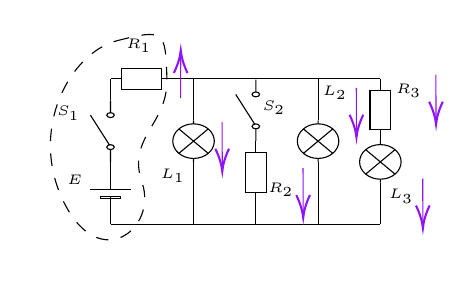
\begin{tikzpicture}[x=0.75pt,y=0.75pt,yscale=-1,xscale=1]
%uncomment if require: \path (0,300); %set diagram left start at 0, and has height of 300

%Shape: Battery [id:dp797984114545808] 
\draw   (100,170) -- (100,156.5) (90,153.5) -- (110,153.5) (100,153.5) -- (100,140) (95,157.7) -- (95,156.5) -- (105,156.5) -- (105,157.7) -- (95,157.7) -- cycle ;
%Shape: Simple Switch [id:dp4334800063265021] 
\draw   (100,140) -- (100,134.07) (100,116.29) -- (100,110.37) (99.39,131.7) -- (90.32,117.48) (100,118.66) .. controls (99,118.66) and (98.18,118.13) .. (98.18,117.48) .. controls (98.18,116.82) and (99,116.29) .. (100,116.29) .. controls (101,116.29) and (101.82,116.82) .. (101.82,117.48) .. controls (101.82,118.13) and (101,118.66) .. (100,118.66) -- cycle (100,134.07) .. controls (99,134.07) and (98.18,133.54) .. (98.18,132.89) .. controls (98.18,132.23) and (99,131.7) .. (100,131.7) .. controls (101,131.7) and (101.82,132.23) .. (101.82,132.89) .. controls (101.82,133.54) and (101,134.07) .. (100,134.07) -- cycle ;
%Shape: Resistor [id:dp901312688402967] 
\draw   (105.4,95) -- (124.6,95) -- (124.6,105) -- (105.4,105) -- (105.4,95) -- cycle (100,100) -- (105.4,100) (124.6,100) -- (130,100) ;
%Straight Lines [id:da2657385353492341] 
\draw    (100,110) -- (100,100) ;
%Straight Lines [id:da5416440059996896] 
\draw    (100,100) ;
%Shape: Light Bulb [id:dp598022898779403] 
\draw   (140,138.33) .. controls (134.48,138.33) and (130,134.6) .. (130,130) .. controls (130,125.4) and (134.48,121.67) .. (140,121.67) .. controls (145.52,121.67) and (150,125.4) .. (150,130) .. controls (150,134.6) and (145.52,138.33) .. (140,138.33) -- cycle (132.88,135.93) -- (147.12,124.07) (132.88,124.07) -- (147.12,135.93) (140,140) -- (140,138.33) (140,121.67) -- (140,120) ;
%Straight Lines [id:da4277642056179305] 
\draw    (140,100) -- (140,120) ;
%Straight Lines [id:da9223803374157449] 
\draw    (100,170) -- (230,170) ;
%Straight Lines [id:da4800046187933087] 
\draw    (140,140) -- (140,170) ;
%Straight Lines [id:da5325118901733754] 
\draw    (130,100) -- (230,100) ;
%Shape: Light Bulb [id:dp8429011424978414] 
\draw   (200,138.33) .. controls (194.48,138.33) and (190,134.6) .. (190,130) .. controls (190,125.4) and (194.48,121.67) .. (200,121.67) .. controls (205.52,121.67) and (210,125.4) .. (210,130) .. controls (210,134.6) and (205.52,138.33) .. (200,138.33) -- cycle (192.88,135.93) -- (207.12,124.07) (192.88,124.07) -- (207.12,135.93) (200,140) -- (200,138.33) (200,121.67) -- (200,120) ;
%Straight Lines [id:da06826023906061329] 
\draw    (200,100) -- (200,120) ;
%Straight Lines [id:da15676855229008013] 
\draw    (200,140) -- (200,170) ;
%Shape: Simple Switch [id:dp5417474493250272] 
\draw   (170,130) -- (170,124.07) (170,106.29) -- (170,100.37) (169.39,121.7) -- (160.32,107.48) (170,108.66) .. controls (169,108.66) and (168.18,108.13) .. (168.18,107.48) .. controls (168.18,106.82) and (169,106.29) .. (170,106.29) .. controls (171,106.29) and (171.82,106.82) .. (171.82,107.48) .. controls (171.82,108.13) and (171,108.66) .. (170,108.66) -- cycle (170,124.07) .. controls (169,124.07) and (168.18,123.54) .. (168.18,122.89) .. controls (168.18,122.23) and (169,121.7) .. (170,121.7) .. controls (171,121.7) and (171.82,122.23) .. (171.82,122.89) .. controls (171.82,123.54) and (171,124.07) .. (170,124.07) -- cycle ;
%Shape: Resistor [id:dp5887325110380754] 
\draw   (165,154.6) -- (165,135.4) -- (175,135.4) -- (175,154.6) -- (165,154.6) -- cycle (170,160) -- (170,154.6) (170,135.4) -- (170,130) ;
%Straight Lines [id:da997349339495381] 
\draw    (170,160) -- (170,170) ;
%Straight Lines [id:da908902191522615] 
\draw    (230,150) -- (230,170) ;
%Shape: Light Bulb [id:dp15511171823131908] 
\draw   (230,148.33) .. controls (224.48,148.33) and (220,144.6) .. (220,140) .. controls (220,135.4) and (224.48,131.67) .. (230,131.67) .. controls (235.52,131.67) and (240,135.4) .. (240,140) .. controls (240,144.6) and (235.52,148.33) .. (230,148.33) -- cycle (222.88,145.93) -- (237.12,134.07) (222.88,134.07) -- (237.12,145.93) (230,150) -- (230,148.33) (230,131.67) -- (230,130) ;
%Shape: Resistor [id:dp2189689923867002] 
\draw   (225,124.6) -- (225,105.4) -- (235,105.4) -- (235,124.6) -- (225,124.6) -- cycle (230,130) -- (230,124.6) (230,105.4) -- (230,100) ;
%Shape: Polygon Curved [id:ds9951042770971332] 
\draw  [dash pattern={on 4.5pt off 4.5pt}] (103.2,81.6) .. controls (126.4,75.6) and (126.37,77.19) .. (127.17,99.59) .. controls (127.97,121.99) and (107.6,128) .. (115.2,150) .. controls (122.8,172) and (94.85,194.15) .. (77.6,159.6) .. controls (60.35,125.05) and (80,87.6) .. (103.2,81.6) -- cycle ;
%Straight Lines [id:da43974811049545215] 
\draw [color={rgb, 255:red, 144; green, 19; blue, 254 }  ,draw opacity=1 ]   (192.75,143) -- (192.83,164.92) ;
\draw [shift={(192.84,166.92)}, rotate = 269.79] [color={rgb, 255:red, 144; green, 19; blue, 254 }  ,draw opacity=1 ][line width=0.75]    (10.93,-3.29) .. controls (6.95,-1.4) and (3.31,-0.3) .. (0,0) .. controls (3.31,0.3) and (6.95,1.4) .. (10.93,3.29)   ;
%Straight Lines [id:da6028004259046089] 
\draw [color={rgb, 255:red, 144; green, 19; blue, 254 }  ,draw opacity=1 ]   (218.41,104.33) -- (218.5,126.25) ;
\draw [shift={(218.5,128.25)}, rotate = 269.79] [color={rgb, 255:red, 144; green, 19; blue, 254 }  ,draw opacity=1 ][line width=0.75]    (10.93,-3.29) .. controls (6.95,-1.4) and (3.31,-0.3) .. (0,0) .. controls (3.31,0.3) and (6.95,1.4) .. (10.93,3.29)   ;
%Straight Lines [id:da18779689260168553] 
\draw [color={rgb, 255:red, 144; green, 19; blue, 254 }  ,draw opacity=1 ]   (250.41,148) -- (250.5,169.92) ;
\draw [shift={(250.5,171.92)}, rotate = 269.79] [color={rgb, 255:red, 144; green, 19; blue, 254 }  ,draw opacity=1 ][line width=0.75]    (10.93,-3.29) .. controls (6.95,-1.4) and (3.31,-0.3) .. (0,0) .. controls (3.31,0.3) and (6.95,1.4) .. (10.93,3.29)   ;
%Straight Lines [id:da47575786229871486] 
\draw [color={rgb, 255:red, 144; green, 19; blue, 254 }  ,draw opacity=1 ]   (256.75,98) -- (256.83,119.92) ;
\draw [shift={(256.84,121.92)}, rotate = 269.79] [color={rgb, 255:red, 144; green, 19; blue, 254 }  ,draw opacity=1 ][line width=0.75]    (10.93,-3.29) .. controls (6.95,-1.4) and (3.31,-0.3) .. (0,0) .. controls (3.31,0.3) and (6.95,1.4) .. (10.93,3.29)   ;
%Straight Lines [id:da9611002858605389] 
\draw [color={rgb, 255:red, 144; green, 19; blue, 254 }  ,draw opacity=1 ]   (153.75,120.67) -- (153.83,142.59) ;
\draw [shift={(153.84,144.59)}, rotate = 269.79] [color={rgb, 255:red, 144; green, 19; blue, 254 }  ,draw opacity=1 ][line width=0.75]    (10.93,-3.29) .. controls (6.95,-1.4) and (3.31,-0.3) .. (0,0) .. controls (3.31,0.3) and (6.95,1.4) .. (10.93,3.29)   ;
%Straight Lines [id:da5346762576536745] 
\draw [color={rgb, 255:red, 144; green, 19; blue, 254 }  ,draw opacity=1 ]   (133.75,109.33) -- (133.83,88.25) ;
\draw [shift={(133.84,86.25)}, rotate = 90.22] [color={rgb, 255:red, 144; green, 19; blue, 254 }  ,draw opacity=1 ][line width=0.75]    (10.93,-3.29) .. controls (6.95,-1.4) and (3.31,-0.3) .. (0,0) .. controls (3.31,0.3) and (6.95,1.4) .. (10.93,3.29)   ;

% Text Node
\draw (78,145) node [anchor=north west][inner sep=0.75pt]  [font=\tiny] [align=left] {$\displaystyle E$};
% Text Node
\draw (73,112) node [anchor=north west][inner sep=0.75pt]  [font=\tiny] [align=left] {$\displaystyle S_{1}$};
% Text Node
\draw (172,109.29) node [anchor=north west][inner sep=0.75pt]  [font=\tiny] [align=left] {$\displaystyle S_{2}$};
% Text Node
\draw (106.33,79.67) node [anchor=north west][inner sep=0.75pt]  [font=\tiny] [align=left] {$\displaystyle R_{1}$};
% Text Node
\draw (174.8,148.8) node [anchor=north west][inner sep=0.75pt]  [font=\tiny] [align=left] {$\displaystyle R_{2}$};
% Text Node
\draw (236.33,101) node [anchor=north west][inner sep=0.75pt]  [font=\tiny] [align=left] {$\displaystyle R_{3}$};
% Text Node
\draw (123,142) node [anchor=north west][inner sep=0.75pt]  [font=\tiny] [align=left] {$\displaystyle L_{1}$};
% Text Node
\draw (201,102) node [anchor=north west][inner sep=0.75pt]  [font=\tiny] [align=left] {$\displaystyle L_{2}$};
% Text Node
\draw (233,152) node [anchor=north west][inner sep=0.75pt]  [font=\tiny] [align=left] {$\displaystyle L_{3}$};

\end{tikzpicture}
\end{center}

如图,当$S_2$所在支路电阻减小时,其各部分电压、电流变化根据“串反并同”如图所示。因此B、D错误,C正确。综上所述,答案为C。

\end{ep}

涉及到与电容器有关的电路问题时,我们可以把电容器当成一个理想的电压表,从而使用“串反并同”。\textbf{但需注意,电容器本质上是断路(在直流电路中),因此跟电容器处在同一支路中串联的电阻改变并不影响电容器两端电压!}具体可见如下例题。

\begin{ep}{2014·天津}{}

\begin{center}
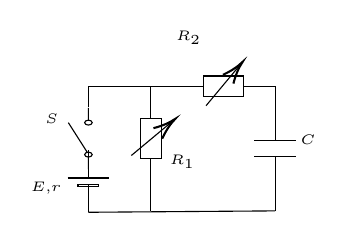
\begin{tikzpicture}[x=0.75pt,y=0.75pt,yscale=-1,xscale=1]
%uncomment if require: \path (0,300); %set diagram left start at 0, and has height of 300

%Shape: Battery [id:dp9725213714143768] 
\draw   (120,180.67) -- (120,167.17) (110,164.17) -- (130,164.17) (120,164.17) -- (120,150.67) (115,168.37) -- (115,167.17) -- (125,167.17) -- (125,168.37) -- (115,168.37) -- cycle ;
%Shape: Simple Switch [id:dp9513460496272634] 
\draw   (120,160) -- (120,154.07) (120,136.29) -- (120,130.37) (119.39,151.7) -- (110.32,137.48) (120,138.66) .. controls (119,138.66) and (118.18,138.13) .. (118.18,137.48) .. controls (118.18,136.82) and (119,136.29) .. (120,136.29) .. controls (121,136.29) and (121.82,136.82) .. (121.82,137.48) .. controls (121.82,138.13) and (121,138.66) .. (120,138.66) -- cycle (120,154.07) .. controls (119,154.07) and (118.18,153.54) .. (118.18,152.89) .. controls (118.18,152.23) and (119,151.7) .. (120,151.7) .. controls (121,151.7) and (121.82,152.23) .. (121.82,152.89) .. controls (121.82,153.54) and (121,154.07) .. (120,154.07) -- cycle ;
%Straight Lines [id:da13406352029154833] 
\draw    (120,130) -- (120,120) ;
%Shape: Resistor [id:dp7782080231234687] 
\draw   (145,154.6) -- (145,135.4) -- (155,135.4) -- (155,154.6) -- (145,154.6) -- cycle (150,160) -- (150,154.6) (150,135.4) -- (150,130) ;
%Straight Lines [id:da13059673417265527] 
\draw    (140.67,153.33) -- (160.3,136.96) ;
\draw [shift={(161.84,135.67)}, rotate = 140.17] [color={rgb, 255:red, 0; green, 0; blue, 0 }  ][line width=0.75]    (10.93,-3.29) .. controls (6.95,-1.4) and (3.31,-0.3) .. (0,0) .. controls (3.31,0.3) and (6.95,1.4) .. (10.93,3.29)   ;

%Straight Lines [id:da15333654490325355] 
\draw    (120,120) -- (170,120) ;
%Straight Lines [id:da8531691012035736] 
\draw    (150,130) -- (150,120) ;
%Straight Lines [id:da4440724028211367] 
\draw    (150,180) -- (150,160) ;
%Shape: Resistor [id:dp2809007889817905] 
\draw   (175.4,125) -- (194.6,125) -- (194.6,115) -- (175.4,115) -- (175.4,125) -- cycle (170,120) -- (175.4,120) (194.6,120) -- (200,120) ;
%Straight Lines [id:da8392657712741902] 
\draw    (176.67,129.33) -- (193.04,109.7) ;
\draw [shift={(194.33,108.16)}, rotate = 129.83] [color={rgb, 255:red, 0; green, 0; blue, 0 }  ][line width=0.75]    (10.93,-3.29) .. controls (6.95,-1.4) and (3.31,-0.3) .. (0,0) .. controls (3.31,0.3) and (6.95,1.4) .. (10.93,3.29)   ;

%Straight Lines [id:da5062655598048114] 
\draw    (200,120) -- (210,120) -- (210,140) ;
%Shape: Contact [id:dp3034505709269577] 
\draw   (210,140) -- (210,146) (210,160) -- (210,154) (220,146) -- (200,146) (220,154) -- (200,154) ;
%Straight Lines [id:da6904084679904827] 
\draw    (210,180) -- (210,160) ;
%Straight Lines [id:da5835108292810021] 
\draw    (120,180.67) -- (210,180) ;

% Text Node
\draw (91,165) node [anchor=north west][inner sep=0.75pt]  [font=\tiny] [align=left] {$\displaystyle E$,$\displaystyle r$};
% Text Node
\draw (98,132) node [anchor=north west][inner sep=0.75pt]  [font=\tiny] [align=left] {$\displaystyle S$};
% Text Node
\draw (158,152) node [anchor=north west][inner sep=0.75pt]  [font=\tiny] [align=left] {$\displaystyle R_{1}$};
% Text Node
\draw (161,92) node [anchor=north west][inner sep=0.75pt]  [font=\tiny] [align=left] {$\displaystyle R_{2}$};
% Text Node
\draw (221,142) node [anchor=north west][inner sep=0.75pt]  [font=\tiny] [align=left] {$\displaystyle C$};


\end{tikzpicture}

\end{center}

如图所示,电路中$R_1$、$R_2$均为可变电阻,电源内阻不能忽
略。平行板电容器$C$的极板水平放置。闭合电键$S$,电路达到稳定时,带电油滴悬浮在两板之间静止不动。如果仅改变下列某一个条件,油滴仍能静止不动的是()

(A) 增大$R_1$的阻值 \quad (B) 增大$R_2$的阻值 \quad (C) 增大两板间的距离 \quad (D) 断开电键$S$

~\\
电阻$R_1$与电容$C$等效并联,增大$R_1$,则$C$两端电压增大,无法保持静止不动,选项A错误。

电阻$R_2$与电容$C$在同一支路上串联,故$R_2$的变化不影响电容$C$两端电压,选项B正确。

增大两板间距离,两板间电压不变,增大距离,电场减弱,无法保持静止不动,选项C错误。

断开$S$,电容两端形成回路放电,无法保持静止不动,选项D错误。综上所述,答案为B。
\end{ep}

这里需要注意,对于分压接法的滑动电阻器,分析滑动电阻器的移动时\textbf{不可直接使用“串反并同”},我们可以将滑动变阻器分成两部分,其中一部分与子电路并联,另一部分与前面并联的部分串联,当移动滑动变阻器时,其并联的电阻跟串联的电阻均发生了变化,\textbf{存在多个电阻变化,违反了“串反并同”的适用条件},故不可直接使用“串反并同”。但我们可以借助戴维宁定理\eqref{dwndl}对子电路进行分析,从而把两个回路建立联系,绕过滑动变阻器进行分析。

当然,\textbf{我们可以把滑动变阻器分成串联部分和并联部分,若有且只有滑动变阻器发生了变化,则滑动变阻器以及整个子电路电阻变化跟串联电阻相同。}

具体操作见下面例题。

\begin{ep}{自编题}{}
\begin{center}
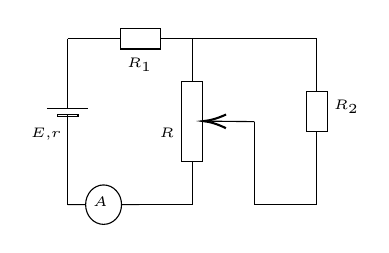
\begin{tikzpicture}[x=0.75pt,y=0.75pt,yscale=-1,xscale=1]
%uncomment if require: \path (0,300); %set diagram left start at 0, and has height of 300

%Straight Lines [id:da9223803374157449] 
\draw    (370,160) -- (430,160) ;
%Straight Lines [id:da4800046187933087] 
\draw    (400,200) -- (400,240) ;
%Straight Lines [id:da15676855229008013] 
\draw    (370,160) -- (370,170) ;
%Shape: Resistor [id:dp5887325110380754] 
\draw   (365,219.2) -- (365,180.8) -- (375,180.8) -- (375,219.2) -- (365,219.2) -- cycle (370,230) -- (370,219.2) (370,180.8) -- (370,170) ;
%Shape: Resistor [id:dp2189689923867002] 
\draw   (425,204.6) -- (425,185.4) -- (435,185.4) -- (435,204.6) -- (425,204.6) -- cycle (430,210) -- (430,204.6) (430,185.4) -- (430,180) ;
%Shape: Battery [id:dp11572428456821915] 
\draw   (310,210) -- (310,196.5) (300,193.5) -- (320,193.5) (310,193.5) -- (310,180) (305,197.7) -- (305,196.5) -- (315,196.5) -- (315,197.7) -- (305,197.7) -- cycle ;
%Straight Lines [id:da5053925872800769] 
\draw    (310,160) -- (310,180) ;
%Shape: Resistor [id:dp8634794872930143] 
\draw   (335.4,155) -- (354.6,155) -- (354.6,165) -- (335.4,165) -- (335.4,155) -- cycle (330,160) -- (335.4,160) (354.6,160) -- (360,160) ;
%Straight Lines [id:da4775642533714568] 
\draw    (310,160) -- (330,160) ;
%Straight Lines [id:da3350904693838317] 
\draw    (360,160) -- (370,160) ;
%Straight Lines [id:da025516599512321214] 
\draw    (310,210) -- (310,240) ;
%Straight Lines [id:da7872440703735311] 
\draw    (370,230) -- (370,240) ;
%Straight Lines [id:da7147480438171852] 
\draw    (400,200) -- (377.34,199.77) ;
\draw [shift={(375.34,199.75)}, rotate = 0.57] [color={rgb, 255:red, 0; green, 0; blue, 0 }  ][line width=0.75]    (10.93,-3.29) .. controls (6.95,-1.4) and (3.31,-0.3) .. (0,0) .. controls (3.31,0.3) and (6.95,1.4) .. (10.93,3.29)   ;
%Shape: Output [id:dp20535874065942084] 
\draw   (318.65,240) .. controls (318.65,234.75) and (322.52,230.5) .. (327.3,230.5) .. controls (332.08,230.5) and (335.95,234.75) .. (335.95,240) .. controls (335.95,245.25) and (332.08,249.5) .. (327.3,249.5) .. controls (322.52,249.5) and (318.65,245.25) .. (318.65,240) -- cycle (310,240) -- (318.65,240) (344.6,240) -- (335.95,240) ;
%Straight Lines [id:da8691520573396538] 
\draw    (340,240) -- (370,240) ;
%Straight Lines [id:da90607602119505] 
\draw    (430,160) -- (430,180) ;
%Straight Lines [id:da522190466993206] 
\draw    (430,210) -- (430,240) ;
%Straight Lines [id:da22747916883790165] 
\draw    (400,240) -- (430,240) ;

% Text Node
\draw (291,202) node [anchor=north west][inner sep=0.75pt]  [font=\tiny] [align=left] {$\displaystyle \ms E$,$\displaystyle r$};
% Text Node
\draw (337.4,168) node [anchor=north west][inner sep=0.75pt]  [font=\tiny] [align=left] {$\displaystyle R_{1}$};
% Text Node
\draw (437,188.4) node [anchor=north west][inner sep=0.75pt]  [font=\tiny] [align=left] {$\displaystyle R_{2}$};
% Text Node
\draw (321,235) node [anchor=north west][inner sep=0.75pt]  [font=\tiny] [align=left] {$\displaystyle A$};
% Text Node
\draw (353,201.67) node [anchor=north west][inner sep=0.75pt]  [font=\tiny] [align=left] {$\displaystyle R$};


\end{tikzpicture}

\end{center}
如图所示电路,内阻不可忽略。现将滑动变阻器$R$的滑片下移,试分析$R_1$、$R_2$两端电压以及电流表$A$的示数$I_A$变化。

~\\
滑片下移,$R$分出的电压更大,即对于子电路而言,电阻$R_2$两端电压增加,电流增加。故通过滑动变阻器$R$的电流增加,滑动变阻器以及子电路等效的电阻减小。由串反并同知$R_1$两端电压增大,电流表$A$示数变大。

当然,由于只有滑动变阻器发生了改变,滑片下移,$R$分出的电压更大,即对于子电路而言,电阻$R_2$两端电压增加,电流增加。滑片下移,其串联部分电阻减小,滑动变阻器以及子电路电阻减小,由串反并同知$R_1$两端电压增大,电流表$A$示数变大。

\end{ep}

\section{变压器等效}

对于变压器问题,一般的方法是对变压器两端列电压方程,再在两个回路中列电学方程,联立求解,这种方法一般会涉及到较多方程的联立,对于选择题等分析判断并不方便,并且也不利于运用上文的“串反并同”\eqref{s_cfbt}。因此,可以通过变压器等效,将其中一个回路等效到另一个回路,从而将一个涉及变压器的双回路问题简化为单回路问题,从而便于运用“串反并同”,简化分析过程,加快计算。

\section{“均方根值”速求有效值}

在高中,电压和电流的有效值的计算一般而言先假设一电阻,求出一端时间后该电阻发热,再假设其等效的电压或电流值,计算该电阻在相同时间内的发热,两者相等,联立消去假设的电阻和时间,求解出等效电压或者电流值。这个方法准确的描述了有效值的定义,但并不利于计算。运用均方根值\footnote{“均方根值”本质上跟数学上的“幂平均值”相同,但在电学分析中一般称其为“均方根值”}以及正弦波与方波的等效可以便捷地求出高中内任意波形的有效值。

\begin{defi}{均方根值}{}

对于一组数$x_1$、$x_2$ ... $x_i$以及其对应的权重$a_1$、$a_2$ ... $a_i$,其均方根值\footnote{rms为均方根值缩写。对于均方根值严格的定义为在一个周期内,$x_{rms} = \sqrt{\frac{1}{T} \int_0^T f(t) dt}$,若$f(t)$对应方波,则可得到离散的上式;对于正弦波的处理,见下文}为

$$x_{rms} = \sqrt{\sum a_i x_i^2} = \sqrt{a_1 \cdot x_1^2 + a_2 \cdot x_2^2 + \cdots + a_i \cdot x_i^2}$$

\end{defi}

现在我们来证明均方根值便是有效值\footnote{其实均方根值的定义便是根据有效值而来,与其称其为证明不如称其为验证}

现在假设一个均为方波的电压周期内,其电压$U_i$占时间$t_i$,假设这一电压加在某一电阻$R$上,则其一个周期内发热为

$$ Q = \sum \frac{U_i^2}{R} t_i $$

现在假设其等效电压为$U_{eq}$,加在电阻$R$上一个周期的时间,则其发热为

$$ Q = \frac{U_{eq}^2}{R} (\sum t_i)$$

上面两式相等,记一个周期时间$T = \sum t_i $,$a_i$为电压$U_i$在周期内占比,则有

$$U_{eq}^2 = \sum \frac{U_i^2 t_i}{T} = \sum a_i U_i^2$$

故电压的有效值为电压的均方根值。对于电流同理。

\begin{theo}{正弦式交流电有效值}{}
对于正弦式交流电,\textbf{其等效值为峰值的$\frac{1}{\sqrt{2}}$倍}
\end{theo}

对于上述结论,高中课本并未给出证明,但可以通过积分证明上述关系,如下

设有一正弦式电压$U = U_0 \sin (\frac{2 \pi}{T} \cdot t )$其中$T$为该正弦交流电周期,$U_0$为该正弦式交流电振幅。将其通在阻值为$R$的电阻上一个周期,则其发热为

$$Q = \int_0^T \frac{1}{R} U_0^2 \sin^2 (\frac{2 \pi}{T} \cdot t ) dt = \frac{U_0^2}{R} \frac{T}{2 \pi} \int_0^{2 \pi} \sin^2 \theta d \theta = \frac{U_0^2 T}{2R}$$

现在假设其等效电压为$U_{eq}$,加在电阻$R$上一个周期的时间,则其发热为

$$ Q = \frac{U_{eq}^2 T}{R} $$

上面两式相等,则有$U_{eq} = \frac{U_0}{\sqrt{2}}$。上述推到对于电流同理,即正弦式交流电等效值为峰值的$\frac{1}{\sqrt{2}}$倍,QED。

\begin{theo}[label=zxbdxfb]{正弦交流电等效方波}{}
对于正弦式交流电,由于$\frac{U_0^2 t}{2} = U_{eq} t$,因此\textbf{对于一个持续时间为$t$、峰值为$U_0$正弦式交流电,其可以用一个电压为$U_0$,持续时间为$\frac{t}{2}$的恒定方波替代(电流同理)}\footnote{这里要求该正弦式交流电满足$\frac{T}{4}$的整数倍,在高中阶段大多满足。由于不满足此条件超出了高中阶段能求解的范围,故笔者目前仍未见到不能运用此方法等效的高中题目。但为了严谨起见,仍旧在此说明一下}。
\end{theo}

\begin{center}
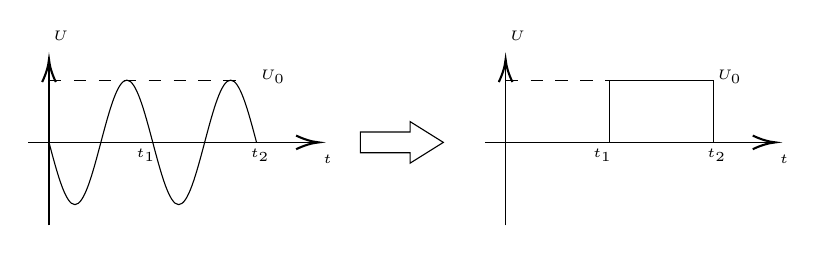
\begin{tikzpicture}[x=0.75pt,y=0.75pt,yscale=-1,xscale=1]
%uncomment if require: \path (0,300); %set diagram left start at 0, and has height of 300

%Shape: Wave [id:dp5957275904614414] 
\draw   (40,100) .. controls (44.08,115.37) and (47.98,130) .. (52.5,130) .. controls (57.02,130) and (60.92,115.37) .. (65,100) .. controls (69.08,84.63) and (72.98,70) .. (77.5,70) .. controls (82.02,70) and (85.92,84.63) .. (90,100) .. controls (94.08,115.37) and (97.98,130) .. (102.5,130) .. controls (107.02,130) and (110.92,115.37) .. (115,100) .. controls (119.08,84.63) and (122.98,70) .. (127.5,70) .. controls (132.02,70) and (135.92,84.63) .. (140,100) ;
%Straight Lines [id:da8807380521016539] 
\draw    (30,100) -- (168,100) ;
\draw [shift={(170,100)}, rotate = 180] [color={rgb, 255:red, 0; green, 0; blue, 0 }  ][line width=0.75]    (10.93,-3.29) .. controls (6.95,-1.4) and (3.31,-0.3) .. (0,0) .. controls (3.31,0.3) and (6.95,1.4) .. (10.93,3.29)   ;
%Straight Lines [id:da7234210438419781] 
\draw    (40,140) -- (40,62) ;
\draw [shift={(40,60)}, rotate = 90] [color={rgb, 255:red, 0; green, 0; blue, 0 }  ][line width=0.75]    (10.93,-3.29) .. controls (6.95,-1.4) and (3.31,-0.3) .. (0,0) .. controls (3.31,0.3) and (6.95,1.4) .. (10.93,3.29)   ;
%Straight Lines [id:da8881692477795176] 
\draw  [dash pattern={on 4.5pt off 4.5pt}]  (40,70) -- (130,70) ;
%Straight Lines [id:da7037740098329359] 
\draw    (250,100) -- (388,100) ;
\draw [shift={(390,100)}, rotate = 180] [color={rgb, 255:red, 0; green, 0; blue, 0 }  ][line width=0.75]    (10.93,-3.29) .. controls (6.95,-1.4) and (3.31,-0.3) .. (0,0) .. controls (3.31,0.3) and (6.95,1.4) .. (10.93,3.29)   ;
%Straight Lines [id:da24696901338014343] 
\draw    (260,140) -- (260,62) ;
\draw [shift={(260,60)}, rotate = 90] [color={rgb, 255:red, 0; green, 0; blue, 0 }  ][line width=0.75]    (10.93,-3.29) .. controls (6.95,-1.4) and (3.31,-0.3) .. (0,0) .. controls (3.31,0.3) and (6.95,1.4) .. (10.93,3.29)   ;
%Straight Lines [id:da028807109360900807] 
\draw  [dash pattern={on 4.5pt off 4.5pt}]  (260,70) -- (350,70) ;
%Right Arrow [id:dp35127513802390187] 
\draw   (190,95) -- (214,95) -- (214,90) -- (230,100) -- (214,110) -- (214,105) -- (190,105) -- cycle ;
%Straight Lines [id:da6668988615484821] 
\draw    (310,70) -- (310,100) ;
%Straight Lines [id:da5154013723623756] 
\draw    (360,70) -- (360,100) ;
%Straight Lines [id:da6769085058841795] 
\draw    (310,70) -- (360,70) ;

% Text Node
\draw (171,105) node [anchor=north west][inner sep=0.75pt]  [font=\tiny] [align=left] {$\displaystyle t$};
% Text Node
\draw (41,45) node [anchor=north west][inner sep=0.75pt]  [font=\tiny] [align=left] {$\displaystyle U$};
% Text Node
\draw (141,64) node [anchor=north west][inner sep=0.75pt]  [font=\tiny] [align=left] {$\displaystyle U_{0}$};
% Text Node
\draw (391,105) node [anchor=north west][inner sep=0.75pt]  [font=\tiny] [align=left] {$\displaystyle t$};
% Text Node
\draw (261,45) node [anchor=north west][inner sep=0.75pt]  [font=\tiny] [align=left] {$\displaystyle U$};
% Text Node
\draw (361,64) node [anchor=north west][inner sep=0.75pt]  [font=\tiny] [align=left] {$\displaystyle U_{0}$};
% Text Node
\draw (81,102) node [anchor=north west][inner sep=0.75pt]  [font=\tiny] [align=left] {$\displaystyle t_{1}$};
% Text Node
\draw (136,102) node [anchor=north west][inner sep=0.75pt]  [font=\tiny] [align=left] {$\displaystyle t_{2}$};
% Text Node
\draw (301,102) node [anchor=north west][inner sep=0.75pt]  [font=\tiny] [align=left] {$\displaystyle t_{1}$};
% Text Node
\draw (356,102) node [anchor=north west][inner sep=0.75pt]  [font=\tiny] [align=left] {$\displaystyle t_{2}$};


\end{tikzpicture}

\end{center}

运用以上方法,我们可以快速计算高中范围内所能见到的电压和电流的有效值,具体操作见下面例题。

\begin{ep}{自编题}{}
现有一交流电,其单个周期内波形如图所示,求该交流电有效值

\begin{center}
\begin{tikzpicture}[x=0.75pt,y=0.75pt,yscale=-1,xscale=1]
%uncomment if require: \path (0,300); %set diagram left start at 0, and has height of 300

%Shape: Wave [id:dp5957275904614414] 
\draw   (40,100) .. controls (44.89,115.37) and (49.57,130) .. (55,130) .. controls (60.43,130) and (65.11,115.37) .. (70,100) .. controls (74.89,84.63) and (79.57,70) .. (85,70) .. controls (90.43,70) and (95.11,84.63) .. (100,100) ;
%Straight Lines [id:da8807380521016539] 
\draw    (30,100) -- (167.3,100) -- (218,100) ;
\draw [shift={(220,100)}, rotate = 180] [color={rgb, 255:red, 0; green, 0; blue, 0 }  ][line width=0.75]    (10.93,-3.29) .. controls (6.95,-1.4) and (3.31,-0.3) .. (0,0) .. controls (3.31,0.3) and (6.95,1.4) .. (10.93,3.29)   ;
%Straight Lines [id:da7234210438419781] 
\draw    (40,160) -- (40,42) ;
\draw [shift={(40,40)}, rotate = 90] [color={rgb, 255:red, 0; green, 0; blue, 0 }  ][line width=0.75]    (10.93,-3.29) .. controls (6.95,-1.4) and (3.31,-0.3) .. (0,0) .. controls (3.31,0.3) and (6.95,1.4) .. (10.93,3.29)   ;
%Straight Lines [id:da8881692477795176] 
\draw  [dash pattern={on 4.5pt off 4.5pt}]  (40,70) -- (150,70) ;
%Straight Lines [id:da4109302093413363] 
\draw    (100,100) -- (100,160) ;
%Straight Lines [id:da7251683684825969] 
\draw    (100,160) -- (115.63,160) -- (130,160) ;
%Straight Lines [id:da6247280744273678] 
\draw  [dash pattern={on 4.5pt off 4.5pt}]  (40,160) -- (100,160) ;
%Straight Lines [id:da4811824903906994] 
\draw    (130,70) -- (130,160) ;
%Straight Lines [id:da07707215432170345] 
\draw    (130,70) -- (160,70) ;
%Straight Lines [id:da7362129417956969] 
\draw    (160,70) -- (160,100) ;

% Text Node
\draw (211,105) node [anchor=north west][inner sep=0.75pt]  [font=\tiny] [align=left] {$\displaystyle t/s$};
% Text Node
\draw (22,22) node [anchor=north west][inner sep=0.75pt]  [font=\tiny] [align=left] {$\displaystyle U/V$};
% Text Node
\draw (22,62) node [anchor=north west][inner sep=0.75pt]  [font=\tiny] [align=left] {$\displaystyle 1V$};
% Text Node
\draw (92,103) node [anchor=north west][inner sep=0.75pt]  [font=\tiny] [align=left] {$\displaystyle 1$};
% Text Node
\draw (161,102) node [anchor=north west][inner sep=0.75pt]  [font=\tiny] [align=left] {$\displaystyle 2$};
% Text Node
\draw (15,152) node [anchor=north west][inner sep=0.75pt]  [font=\tiny] [align=left] {$\displaystyle -2V$};
% Text Node
\draw (111,85) node [anchor=north west][inner sep=0.75pt]  [font=\tiny] [align=left] {$\displaystyle 1.5$};
% Text Node
\draw (52,85) node [anchor=north west][inner sep=0.75pt]  [font=\tiny] [align=left] {$\displaystyle 0.5$};


\end{tikzpicture}

\end{center}

首先,我们先把正弦波等效为方波,根据前文定理\eqref{zxbdxfb},有

\begin{center}
\begin{tikzpicture}[x=0.75pt,y=0.75pt,yscale=-1,xscale=1]
%uncomment if require: \path (0,300); %set diagram left start at 0, and has height of 300

%Shape: Wave [id:dp5957275904614414] 
\draw   (40,100) .. controls (44.89,115.37) and (49.57,130) .. (55,130) .. controls (60.43,130) and (65.11,115.37) .. (70,100) .. controls (74.89,84.63) and (79.57,70) .. (85,70) .. controls (90.43,70) and (95.11,84.63) .. (100,100) ;
%Straight Lines [id:da8807380521016539] 
\draw    (30,100) -- (167.3,100) -- (218,100) ;
\draw [shift={(220,100)}, rotate = 180] [color={rgb, 255:red, 0; green, 0; blue, 0 }  ][line width=0.75]    (10.93,-3.29) .. controls (6.95,-1.4) and (3.31,-0.3) .. (0,0) .. controls (3.31,0.3) and (6.95,1.4) .. (10.93,3.29)   ;
%Straight Lines [id:da7234210438419781] 
\draw    (40,160) -- (40,42) ;
\draw [shift={(40,40)}, rotate = 90] [color={rgb, 255:red, 0; green, 0; blue, 0 }  ][line width=0.75]    (10.93,-3.29) .. controls (6.95,-1.4) and (3.31,-0.3) .. (0,0) .. controls (3.31,0.3) and (6.95,1.4) .. (10.93,3.29)   ;
%Straight Lines [id:da8881692477795176] 
\draw  [dash pattern={on 4.5pt off 4.5pt}]  (40,70) -- (150,70) ;
%Straight Lines [id:da4109302093413363] 
\draw    (100,100) -- (100,160) ;
%Straight Lines [id:da7251683684825969] 
\draw    (100,160) -- (115.63,160) -- (130,160) ;
%Straight Lines [id:da6247280744273678] 
\draw  [dash pattern={on 4.5pt off 4.5pt}]  (40,160) -- (100,160) ;
%Straight Lines [id:da4811824903906994] 
\draw    (130,70) -- (130,160) ;
%Straight Lines [id:da07707215432170345] 
\draw    (130,70) -- (160,70) ;
%Straight Lines [id:da7362129417956969] 
\draw    (160,70) -- (160,100) ;
%Right Arrow [id:dp2964750951442603] 
\draw   (250,97.5) -- (292,97.5) -- (292,90) -- (320,105) -- (292,120) -- (292,112.5) -- (250,112.5) -- cycle ;
%Straight Lines [id:da09767427738803702] 
\draw    (350,100) -- (487.3,100) -- (538,100) ;
\draw [shift={(540,100)}, rotate = 180] [color={rgb, 255:red, 0; green, 0; blue, 0 }  ][line width=0.75]    (10.93,-3.29) .. controls (6.95,-1.4) and (3.31,-0.3) .. (0,0) .. controls (3.31,0.3) and (6.95,1.4) .. (10.93,3.29)   ;
%Straight Lines [id:da14812927937967957] 
\draw    (360,160) -- (360,42) ;
\draw [shift={(360,40)}, rotate = 90] [color={rgb, 255:red, 0; green, 0; blue, 0 }  ][line width=0.75]    (10.93,-3.29) .. controls (6.95,-1.4) and (3.31,-0.3) .. (0,0) .. controls (3.31,0.3) and (6.95,1.4) .. (10.93,3.29)   ;
%Straight Lines [id:da18788096109920538] 
\draw    (420,70) -- (420,160) ;
%Straight Lines [id:da8582172719266195] 
\draw    (420,160) -- (435.63,160) -- (450,160) ;
%Straight Lines [id:da198364716671944] 
\draw  [dash pattern={on 4.5pt off 4.5pt}]  (360,160) -- (420,160) ;
%Straight Lines [id:da052239762684211044] 
\draw    (450,70) -- (450,160) ;
%Straight Lines [id:da06018736260010238] 
\draw    (450,70) -- (480,70) ;
%Straight Lines [id:da6522253327127172] 
\draw    (480,70) -- (480,100) ;
%Straight Lines [id:da41909877434480447] 
\draw    (390,70) -- (390,100) ;
%Straight Lines [id:da42513251191113355] 
\draw    (390,70) -- (420,70) ;
%Straight Lines [id:da6695934984306693] 
\draw  [dash pattern={on 4.5pt off 4.5pt}]  (360,70) -- (390,70) ;

% Text Node
\draw (211,105) node [anchor=north west][inner sep=0.75pt]  [font=\tiny] [align=left] {$\displaystyle t/s$};
% Text Node
\draw (22,22) node [anchor=north west][inner sep=0.75pt]  [font=\tiny] [align=left] {$\displaystyle U/V$};
% Text Node
\draw (22,62) node [anchor=north west][inner sep=0.75pt]  [font=\tiny] [align=left] {$\displaystyle 1V$};
% Text Node
\draw (92,103) node [anchor=north west][inner sep=0.75pt]  [font=\tiny] [align=left] {$\displaystyle 1$};
% Text Node
\draw (161,102) node [anchor=north west][inner sep=0.75pt]  [font=\tiny] [align=left] {$\displaystyle 2$};
% Text Node
\draw (15,152) node [anchor=north west][inner sep=0.75pt]  [font=\tiny] [align=left] {$\displaystyle -2V$};
% Text Node
\draw (111,85) node [anchor=north west][inner sep=0.75pt]  [font=\tiny] [align=left] {$\displaystyle 1.5$};
% Text Node
\draw (52,85) node [anchor=north west][inner sep=0.75pt]  [font=\tiny] [align=left] {$\displaystyle 0.5$};
% Text Node
\draw (531,105) node [anchor=north west][inner sep=0.75pt]  [font=\tiny] [align=left] {$\displaystyle t/s$};
% Text Node
\draw (342,22) node [anchor=north west][inner sep=0.75pt]  [font=\tiny] [align=left] {$\displaystyle U/V$};
% Text Node
\draw (342,62) node [anchor=north west][inner sep=0.75pt]  [font=\tiny] [align=left] {$\displaystyle 1V$};
% Text Node
\draw (412,103) node [anchor=north west][inner sep=0.75pt]  [font=\tiny] [align=left] {$\displaystyle 1$};
% Text Node
\draw (481,102) node [anchor=north west][inner sep=0.75pt]  [font=\tiny] [align=left] {$\displaystyle 2$};
% Text Node
\draw (335,152) node [anchor=north west][inner sep=0.75pt]  [font=\tiny] [align=left] {$\displaystyle -2V$};
% Text Node
\draw (431,85) node [anchor=north west][inner sep=0.75pt]  [font=\tiny] [align=left] {$\displaystyle 1.5$};
% Text Node
\draw (372,85) node [anchor=north west][inner sep=0.75pt]  [font=\tiny] [align=left] {$\displaystyle 0.5$};
\end{tikzpicture}
\end{center}

因此,我们可以看到,等效后整个波形由两个电压组成,$1V$电压持续了$1s$,占了整个波形的$\frac{1}{2}$。而$2V$电压(\textbf{计算有效值时我们不考虑正负})持续了$0.5s$,占了整个波形的$\frac{1}{4}$。因此,由均方根值计算公式,有

$$U_{eq} = \sqrt{\frac{1}{2} \times 1^2 + \frac{1}{4} \times 2^2} = \frac{\sqrt{6}}{2}$$

此方法熟练后,如果题目数据设置比较易算,我们可以直接口算出有效值。

\end{ep}

\section{配速法}

\section{正则动量}

\section{电磁场换系}

%# -*- coding: utf-8-unix -*-
%%==================================================
\tikzset{every picture/.style={line width=0.75pt}} %set default line width to 0.75pt    

\chapter{波动与光学}

\section{参考圆}

\section{“同侧法”判断波动方向}

\section{“旋转法”判断干涉平面凸起还是凹下}

\section{双缝干涉 —— “横乘横等于竖乘竖”}

%\subsection{}


\chapter{测试}

\textbf{此章节仅做测试使用,之后删除}

\section{SI单位}

使用\verb+siunitx+宏包可以方便地输入SI单位制单位,例如\verb+\SI{5}{\um}+可以得到\SI{5}{\um}。

\section{定理环境}

在本书中,定义了如下几个环境
mk(注),theo(定理),defi(定义),ep(例),mk(注)。

\begin{theo}{勾股定理}{}
若 $a,b$ 为直角三角形的两条直角边,$c$ 为斜边,那么 $a^2 + b^2 + c^2.$
\end{theo}

\begin{ep}{诗句}{}
似此星辰非昨夜
\end{ep}

\begin{defi}{质心}{}
若各质点质量与坐标分别为$m_1$、$(x_1,y_1)$,$m_2$、$(x_2,y_2)$……$m_n$、$(x_n,y_n)$,则质心位置为
$$x_c = \frac{\sum m_i x_i}{\sum m_i} \quad y_c = \frac{\sum m_i y_i}{\sum m_i}$$
\end{defi}

\begin{mk}{标注}{}
这是一个标注
\end{mk}

\end{document}